%==================================================================================
%==================================================================================
% Document		:		Résumé automatique de textes
%
% Auteur		: 		Abdelkrime ARIES
% Encadreur		:		Dr. Omar NOUALI
% Co-encadreur	:		Mme. Houda OUFAIDA
% Établissement	:		ESI (Ecole Nationale Supérieure d'Informatique; ex. INI) 
% Adresse		:		Oued Smar, Alger, Algérie 
% Année			:		2012/2013
% Grade			:		Magister
% discipline 	:		Informatique 
% Spécialité	:		IRM (Informatique Répartie et Mobile)
% Titre			:		Résumé automatique de textes
%
%==================================================================================
%==================================================================================

%==========================L'entete de chapitre====================================
%==================================================================================
\documentclass[a4paper,12pt,oneside]{use/ESIthesis}

\usepackage{amsmath,amssymb}             % AMS Math
\usepackage[utf8]{inputenc}
%\usepackage[T1]{fontenc} %,LAE 
\usepackage[T1]{fontenc}
%\usepackage[french,english]{babel}
\usepackage[frenchb]{babel}
\usepackage{microtype}

%\usepackage[left=2.5cm,right=2.5cm,top=2.5cm,bottom=2.5cm,includefoot,includehead,headheight=13.6pt]{geometry}
\usepackage[left=2.8cm,right=2.2cm,top=2.8cm,bottom=2.8cm,includefoot,includehead,headheight=13.6pt]{geometry}
%\usepackage[left=3.8cm,right=3.2cm,top=2.8cm,bottom=2.8cm,includefoot,includehead,headheight=13.6pt]{geometry}
%\usepackage[left=1.5in,right=1.3in,top=1.1in,bottom=1.1in,includefoot,includehead,headheight=13.6pt]{geometry}
\renewcommand{\baselinestretch}{1.5}

% Table of contents for each chapter

\usepackage[nottoc, notlof, notlot]{tocbibind}
\usepackage[french]{minitoc}
\setcounter{minitocdepth}{1}
\mtcindent=15pt
% Use \minitoc where to put a table of contents

\usepackage{aecompl}

% Glossary / list of abbreviations

\usepackage[intoc]{nomencl}
%\renewcommand{\nomname}{List of Abbreviations}

\makenomenclature

% My pdf code

\usepackage[pdftex]{graphicx}
\usepackage[a4paper,pagebackref,hyperindex=true]{hyperref}

%I added
%\usepackage{tabulary}
%\usepackage{longtable}
%\usepackage[table]{xcolor}
\usepackage{indentfirst}


% Links in pdf
\usepackage{color}
%\definecolor{linkcol}{rgb}{0,0,0.4} 
%\definecolor{citecol}{rgb}{0.5,0,0} 

% Change this to change the informations included in the pdf file

% See hyperref documentation for information on those parameters

\hypersetup
{
%bookmarksopen=true,
pdftitle=Résumé Automatique de Textes,
pdfauthor=Abdelkrime ARIES, 
pdfsubject= {Résumé automatique de textes en utilisant une approche statistique, le regroupement, et la classification} , %subject of the document
%%pdftoolbar=false, % toolbar hidden
%pdfmenubar=true, %menubar shown
%pdfhighlight=/O, %effect of clicking on a link
colorlinks=false, %couleurs sur les liens hypertextes
%pdfpagemode=None, %aucun mode de page
%pdfpagelayout=SinglePage, %ouverture en simple page
%pdffitwindow=true, %pages ouvertes entierement dans toute la fenetre
%linkcolor=linkcol, %couleur des liens hypertextes internes
%citecolor=citecol, %couleur des liens pour les citations
%urlcolor=linkcol %couleur des liens pour les url
}



% Some useful commands and shortcut for maths:  partial derivative and stuff

\newcommand{\pd}[2]{\frac{\partial #1}{\partial #2}}
\def\abs{\operatorname{abs}}
\def\argmax{\operatornamewithlimits{arg\,max}}
\def\argmin{\operatornamewithlimits{arg\,min}}
\def\diag{\operatorname{Diag}}
\newcommand{\eqRef}[1]{(\ref{#1})}

\usepackage{rotating}                    % Sideways of figures & tables
%\usepackage{bibunits}
%\usepackage[sectionbib]{chapterbib}          % Cross-reference package (Natural BiB)
%\usepackage{natbib}                  % Put References at the end of each chapter
                                         % Do not put 'sectionbib' option here.
                                         % Sectionbib option in 'natbib' will do.
\usepackage{fancyhdr}                    % Fancy Header and Footer

\usepackage{txfonts}                     % Public Times New Roman text & math font
  
%%% Fancy Header %%%%%%%%%%%%%%%%%%%%%%%%%%%%%%%%%%%%%%%%%%%%%%%%%%%%%%%%%%%%%%%%%%
% Fancy Header Style Options

\pagestyle{fancy}                       % Sets fancy header and footer
\fancyfoot{}                            % Delete current footer settings

%\renewcommand{\chaptermark}[1]{         % Lower Case Chapter marker style
%  \markboth{\chaptername\ \thechapter.\ #1}}{}} %

%\renewcommand{\sectionmark}[1]{         % Lower case Section marker style
%  \markright{\thesection.\ #1}}         %
%\fancyhead[LE,RO]{\bfseries\thepage}    % Page number (boldface) in left on even
%										% pages and right on odd pages
%\fancyhead[RE]{\bfseries\nouppercase{\leftmark}}      % Chapter in the right on even pages
%\fancyhead[LO]{\bfseries\nouppercase{\rightmark}}     % Section in the left on odd pages

\fancyhead[R]{\bfseries\thepage}    % Page number (boldface) in right
\fancyhead[L]{\bfseries\nouppercase{\rightmark}}     % Section in the left on odd pages

\let\headruleORIG\headrule
\renewcommand{\headrule}{\color{black} \headruleORIG}
\renewcommand{\headrulewidth}{1.0pt}
\usepackage{colortbl}
\arrayrulecolor{black}

\fancypagestyle{plain}{
  \fancyhead{}
  \fancyfoot{}
  \renewcommand{\headrulewidth}{0pt}
}

%\usepackage{algorithm}
%\usepackage[noend]{algorithmic}

%%% Clear Header %%%%%%%%%%%%%%%%%%%%%%%%%%%%%%%%%%%%%%%%%%%%%%%%%%%%%%%%%%%%%%%%%%
% Clear Header Style on the Last Empty Odd pages
\makeatletter

\def\cleardoublepage{\clearpage\if@twoside \ifodd\c@page\else%
  \hbox{}%
  \thispagestyle{empty}%              % Empty header styles
  \newpage%
  \if@twocolumn\hbox{}\newpage\fi\fi\fi}

\makeatother
 
%%%%%%%%%%%%%%%%%%%%%%%%%%%%%%%%%%%%%%%%%%%%%%%%%%%%%%%%%%%%%%%%%%%%%%%%%%%%%%% 
% Prints your review date and 'Draft Version' (From Josullvn, CS, CMU)
\newcommand{\reviewtimetoday}[2]{\special{!userdict begin
    /bop-hook{gsave 20 710 translate 45 rotate 0.8 setgray
      /Times-Roman findfont 12 scalefont setfont 0 0   moveto (#1) show
      0 -12 moveto (#2) show grestore}def end}}
% You can turn on or off this option.
% \reviewtimetoday{\today}{Draft Version}
%%%%%%%%%%%%%%%%%%%%%%%%%%%%%%%%%%%%%%%%%%%%%%%%%%%%%%%%%%%%%%%%%%%%%%%%%%%%%%% 

\newenvironment{maxime}[1]
{
\vspace*{0cm}
\hfill
\begin{minipage}{0.5\textwidth}%
%\rule[0.5ex]{\textwidth}{0.1mm}\\%
\hrulefill $\:$ {\bf #1}\\
%\vspace*{-0.25cm}
\it 
}%
{%

\hrulefill
\vspace*{0.5cm}%
\end{minipage}
}

\let\minitocORIG\minitoc
\renewcommand{\minitoc}{\minitocORIG \vspace{1.5em}} %1.5em

\usepackage{multirow}
%\usepackage{slashbox}

\newenvironment{bulletList}%
{ \begin{list}%
	{$\bullet$}%
	{\setlength{\labelwidth}{25pt}%
	 \setlength{\leftmargin}{30pt}%
	 \setlength{\itemsep}{\parsep}}}%
{ \end{list} }

\newtheorem{definition}{Définition }
\renewcommand{\epsilon}{\varepsilon}

% centered page environment

\newenvironment{vcenterpage}
{\newpage\vspace*{\fill}\thispagestyle{empty}\renewcommand{\headrulewidth}{0pt}}
{\vspace*{\fill}}

%%%%%%%%%%%%%%%%%%%%%%%%%%%%%%%%%%%%%%%%%%%%%%%%%%%%%%%%%%%%%%%%%%%%
% Par Karim
%%%%%%%%%%%%%%%%%%%%%%%%%%%%%%%%%%%%%%%%%%%%%%%%%%%%%%%%%%%%%%%%%%%%
%for the degree sign
\usepackage{textcomp} 
\usepackage{bookmark}
\usepackage{framed}
\usepackage{arabtex}
%\usepackage{nashbf}
%\usepackage{atrans}
%calligra font for the remerciement
\usepackage{calligra}

%List of acronyms
\usepackage{acronym}

\newcommand{\racine}{./}

\newcommand{\setracine}[1]{\renewcommand{\racine}{#1}}

\newcommand{\tablefile}[1]{\input{\racine tab/#1}}
\newcommand{\appendixfile}[1]{\input{\racine anx/#1}}
%\newcommand{\chapterfile}[1]{\input{\racine chap/#1}}

\newcommand{\stitle}[1]{
\noindent
\textbf{#1}
}

\newenvironment{itemizeb}
{\begin{list}{\textbullet} {\setlength{\rightmargin}{0cm} \setlength{\leftmargin}{1cm}}}
{\end{list}}


\newenvironment{itemizec}
{\begin{list}{\textopenbullet} {\setlength{\rightmargin}{0cm} \setlength{\leftmargin}{1cm}}}
{\end{list}}


\newcommand{\kexpbox}[1]{

\vspace{5mm}
\noindent
 \fbox{%
   \parbox{0.985\linewidth}{%
   \vspace{2mm}
   {\large  \textbf{Exemple:}}\\
      #1
   }%
 }
}

\newcommand{\kbox}[1]{

\vspace{2mm}
\noindent
 \fbox{%
   \parbox{0.965\linewidth}{%
   \vspace{2mm}
      #1
   }%
 }
}

\newenvironment{kexp}
{
\begin{framed}
\noindent
{\large  \textbf{Exemple:}}\\
}
{
\end{framed}
}

%%%%%%%%%%%%%%%%%%%%%%%%%%%%%%%%%%%%%%%%%%%%%%%%%%%%%%%%%%%%%%%%%%%%
%%%%%%%%%%%%%%%%%%%%%%%%%%%%%%%%%%%%%%%%%%%%%%%%%%%%%%%%%%%%%%%%%%%%

% definitions.
% -------------------

\setcounter{secnumdepth}{3}
\setcounter{tocdepth}{2}

\newcommand{\tab}[1]{{\hskip #1}}

\graphicspath{{.}{fig/}}

\newcommand \logoESI{../use/logos/ESI.png}

\let\wholebook=\relax
%==================================================================================

\begin{document}
\selectlanguage{french}
\dominitoc

\pdfbookmark{R\'esum\'e automatique de textes (Page de garde)}{Garde}
\ifx\wholebook\relax\else
% --------------------------------------------
% Lulu:
    \documentclass[a4paper,11pt,twoside]{../use/ESIthesis}
	\usepackage{amsmath,amssymb}             % AMS Math
\usepackage[utf8]{inputenc}
%\usepackage[T1]{fontenc} %,LAE 
\usepackage[T1]{fontenc}
%\usepackage[french,english]{babel}
\usepackage[frenchb]{babel}
\usepackage{microtype}

%\usepackage[left=2.5cm,right=2.5cm,top=2.5cm,bottom=2.5cm,includefoot,includehead,headheight=13.6pt]{geometry}
\usepackage[left=2.8cm,right=2.2cm,top=2.8cm,bottom=2.8cm,includefoot,includehead,headheight=13.6pt]{geometry}
%\usepackage[left=3.8cm,right=3.2cm,top=2.8cm,bottom=2.8cm,includefoot,includehead,headheight=13.6pt]{geometry}
%\usepackage[left=1.5in,right=1.3in,top=1.1in,bottom=1.1in,includefoot,includehead,headheight=13.6pt]{geometry}
\renewcommand{\baselinestretch}{1.5}

% Table of contents for each chapter

\usepackage[nottoc, notlof, notlot]{tocbibind}
\usepackage[french]{minitoc}
\setcounter{minitocdepth}{1}
\mtcindent=15pt
% Use \minitoc where to put a table of contents

\usepackage{aecompl}

% Glossary / list of abbreviations

\usepackage[intoc]{nomencl}
%\renewcommand{\nomname}{List of Abbreviations}

\makenomenclature

% My pdf code

\usepackage[pdftex]{graphicx}
\usepackage[a4paper,pagebackref,hyperindex=true]{hyperref}

%I added
%\usepackage{tabulary}
%\usepackage{longtable}
%\usepackage[table]{xcolor}
\usepackage{indentfirst}


% Links in pdf
\usepackage{color}
%\definecolor{linkcol}{rgb}{0,0,0.4} 
%\definecolor{citecol}{rgb}{0.5,0,0} 

% Change this to change the informations included in the pdf file

% See hyperref documentation for information on those parameters

\hypersetup
{
%bookmarksopen=true,
pdftitle=Résumé Automatique de Textes,
pdfauthor=Abdelkrime ARIES, 
pdfsubject= {Résumé automatique de textes en utilisant une approche statistique, le regroupement, et la classification} , %subject of the document
%%pdftoolbar=false, % toolbar hidden
%pdfmenubar=true, %menubar shown
%pdfhighlight=/O, %effect of clicking on a link
colorlinks=false, %couleurs sur les liens hypertextes
%pdfpagemode=None, %aucun mode de page
%pdfpagelayout=SinglePage, %ouverture en simple page
%pdffitwindow=true, %pages ouvertes entierement dans toute la fenetre
%linkcolor=linkcol, %couleur des liens hypertextes internes
%citecolor=citecol, %couleur des liens pour les citations
%urlcolor=linkcol %couleur des liens pour les url
}



% Some useful commands and shortcut for maths:  partial derivative and stuff

\newcommand{\pd}[2]{\frac{\partial #1}{\partial #2}}
\def\abs{\operatorname{abs}}
\def\argmax{\operatornamewithlimits{arg\,max}}
\def\argmin{\operatornamewithlimits{arg\,min}}
\def\diag{\operatorname{Diag}}
\newcommand{\eqRef}[1]{(\ref{#1})}

\usepackage{rotating}                    % Sideways of figures & tables
%\usepackage{bibunits}
%\usepackage[sectionbib]{chapterbib}          % Cross-reference package (Natural BiB)
%\usepackage{natbib}                  % Put References at the end of each chapter
                                         % Do not put 'sectionbib' option here.
                                         % Sectionbib option in 'natbib' will do.
\usepackage{fancyhdr}                    % Fancy Header and Footer

\usepackage{txfonts}                     % Public Times New Roman text & math font
  
%%% Fancy Header %%%%%%%%%%%%%%%%%%%%%%%%%%%%%%%%%%%%%%%%%%%%%%%%%%%%%%%%%%%%%%%%%%
% Fancy Header Style Options

\pagestyle{fancy}                       % Sets fancy header and footer
\fancyfoot{}                            % Delete current footer settings

%\renewcommand{\chaptermark}[1]{         % Lower Case Chapter marker style
%  \markboth{\chaptername\ \thechapter.\ #1}}{}} %

%\renewcommand{\sectionmark}[1]{         % Lower case Section marker style
%  \markright{\thesection.\ #1}}         %
%\fancyhead[LE,RO]{\bfseries\thepage}    % Page number (boldface) in left on even
%										% pages and right on odd pages
%\fancyhead[RE]{\bfseries\nouppercase{\leftmark}}      % Chapter in the right on even pages
%\fancyhead[LO]{\bfseries\nouppercase{\rightmark}}     % Section in the left on odd pages

\fancyhead[R]{\bfseries\thepage}    % Page number (boldface) in right
\fancyhead[L]{\bfseries\nouppercase{\rightmark}}     % Section in the left on odd pages

\let\headruleORIG\headrule
\renewcommand{\headrule}{\color{black} \headruleORIG}
\renewcommand{\headrulewidth}{1.0pt}
\usepackage{colortbl}
\arrayrulecolor{black}

\fancypagestyle{plain}{
  \fancyhead{}
  \fancyfoot{}
  \renewcommand{\headrulewidth}{0pt}
}

%\usepackage{algorithm}
%\usepackage[noend]{algorithmic}

%%% Clear Header %%%%%%%%%%%%%%%%%%%%%%%%%%%%%%%%%%%%%%%%%%%%%%%%%%%%%%%%%%%%%%%%%%
% Clear Header Style on the Last Empty Odd pages
\makeatletter

\def\cleardoublepage{\clearpage\if@twoside \ifodd\c@page\else%
  \hbox{}%
  \thispagestyle{empty}%              % Empty header styles
  \newpage%
  \if@twocolumn\hbox{}\newpage\fi\fi\fi}

\makeatother
 
%%%%%%%%%%%%%%%%%%%%%%%%%%%%%%%%%%%%%%%%%%%%%%%%%%%%%%%%%%%%%%%%%%%%%%%%%%%%%%% 
% Prints your review date and 'Draft Version' (From Josullvn, CS, CMU)
\newcommand{\reviewtimetoday}[2]{\special{!userdict begin
    /bop-hook{gsave 20 710 translate 45 rotate 0.8 setgray
      /Times-Roman findfont 12 scalefont setfont 0 0   moveto (#1) show
      0 -12 moveto (#2) show grestore}def end}}
% You can turn on or off this option.
% \reviewtimetoday{\today}{Draft Version}
%%%%%%%%%%%%%%%%%%%%%%%%%%%%%%%%%%%%%%%%%%%%%%%%%%%%%%%%%%%%%%%%%%%%%%%%%%%%%%% 

\newenvironment{maxime}[1]
{
\vspace*{0cm}
\hfill
\begin{minipage}{0.5\textwidth}%
%\rule[0.5ex]{\textwidth}{0.1mm}\\%
\hrulefill $\:$ {\bf #1}\\
%\vspace*{-0.25cm}
\it 
}%
{%

\hrulefill
\vspace*{0.5cm}%
\end{minipage}
}

\let\minitocORIG\minitoc
\renewcommand{\minitoc}{\minitocORIG \vspace{1.5em}} %1.5em

\usepackage{multirow}
%\usepackage{slashbox}

\newenvironment{bulletList}%
{ \begin{list}%
	{$\bullet$}%
	{\setlength{\labelwidth}{25pt}%
	 \setlength{\leftmargin}{30pt}%
	 \setlength{\itemsep}{\parsep}}}%
{ \end{list} }

\newtheorem{definition}{Définition }
\renewcommand{\epsilon}{\varepsilon}

% centered page environment

\newenvironment{vcenterpage}
{\newpage\vspace*{\fill}\thispagestyle{empty}\renewcommand{\headrulewidth}{0pt}}
{\vspace*{\fill}}

%%%%%%%%%%%%%%%%%%%%%%%%%%%%%%%%%%%%%%%%%%%%%%%%%%%%%%%%%%%%%%%%%%%%
% Par Karim
%%%%%%%%%%%%%%%%%%%%%%%%%%%%%%%%%%%%%%%%%%%%%%%%%%%%%%%%%%%%%%%%%%%%
%for the degree sign
\usepackage{textcomp} 
\usepackage{bookmark}
\usepackage{framed}
\usepackage{arabtex}
%\usepackage{nashbf}
%\usepackage{atrans}
%calligra font for the remerciement
\usepackage{calligra}

%List of acronyms
\usepackage{acronym}

\newcommand{\racine}{./}

\newcommand{\setracine}[1]{\renewcommand{\racine}{#1}}

\newcommand{\tablefile}[1]{\input{\racine tab/#1}}
\newcommand{\appendixfile}[1]{\input{\racine anx/#1}}
%\newcommand{\chapterfile}[1]{\input{\racine chap/#1}}

\newcommand{\stitle}[1]{
\noindent
\textbf{#1}
}

\newenvironment{itemizeb}
{\begin{list}{\textbullet} {\setlength{\rightmargin}{0cm} \setlength{\leftmargin}{1cm}}}
{\end{list}}


\newenvironment{itemizec}
{\begin{list}{\textopenbullet} {\setlength{\rightmargin}{0cm} \setlength{\leftmargin}{1cm}}}
{\end{list}}


\newcommand{\kexpbox}[1]{

\vspace{5mm}
\noindent
 \fbox{%
   \parbox{0.985\linewidth}{%
   \vspace{2mm}
   {\large  \textbf{Exemple:}}\\
      #1
   }%
 }
}

\newcommand{\kbox}[1]{

\vspace{2mm}
\noindent
 \fbox{%
   \parbox{0.965\linewidth}{%
   \vspace{2mm}
      #1
   }%
 }
}

\newenvironment{kexp}
{
\begin{framed}
\noindent
{\large  \textbf{Exemple:}}\\
}
{
\end{framed}
}

%%%%%%%%%%%%%%%%%%%%%%%%%%%%%%%%%%%%%%%%%%%%%%%%%%%%%%%%%%%%%%%%%%%%
%%%%%%%%%%%%%%%%%%%%%%%%%%%%%%%%%%%%%%%%%%%%%%%%%%%%%%%%%%%%%%%%%%%%

% definitions.
% -------------------

\setcounter{secnumdepth}{3}
\setcounter{tocdepth}{2}

\newcommand{\tab}[1]{{\hskip #1}}
	\newcommand \logoESI{../use/logos/ESI.png}
	\graphicspath{{.}{../figures/}}

	\begin{document}
\fi

\begin{titlepage}

\ThesisTitle{R\'{e}sum\'{e} automatique de textes} 
\ThesisKind{M\'EMOIRE}
\ThesisPresentedThe{Pr\'esent\'e et soutenu publiquement le 26/06/2013}
%\ThesisSubTitle{Utilisation de Regroupemnt et de classification pour le score} 
%\ThesisDate{the date of defence}
%\ThesisLoc{l'ESI}
\ThesisAuthor{ARIES Abdelkrime} 
\ThesisESI

% Jury: 
\President = {M. HIDOUCI Walid Khaled \tab{1em}  M.C.A \tab{1em} ESI} 
%\Rapporteurs = {
%Reviewer 1 \\
%Reviewer 2
%} 
\Examinateurs = {
M. CHALAL Rachid \tab{4em} M.C.A  \tab{1em}  ESI \\
M. BOUHADADA Tahar \tab{2em} M.C.A \tab{1em} Université d’Annaba
} 
\Directeur = {M. NOUALI Omar \tab{5em} D.R \tab{2em} CERIST}
%\Coencadreur = {Houda OUFAIDA}

\MakeThesisTitlePage 

\end{titlepage}

%\begin{titlepage}
%\begin{center}
%\noindent {\large \textbf{Universit\'e des Sciences et Technologies de Lille -- Lille 1}} \\2
%\vspace*{0.3cm}
%\noindent {\LARGE \textbf{\'Ecole doctorale SPI Lille}} \\
%\noindent \textbf{D\'epartement de formation doctorale en informatique} \\
%\vspace*{0.5cm}
%\noindent \Huge \textbf{P H D\ \ T H E S I S} \\
%\vspace*{0.3cm}
%\noindent \large {pour l'obtention du} \\
%\vspace*{0.3cm}
%\noindent \LARGE \textbf{Doctorat en science} \\
%\vspace*{0.3cm}
%\noindent \Large de l'Universit\'e des Sciences et Technologies de Lille \\
%\noindent \Large \textbf{Specialt\'e : \textsc{Informatique}}\\
%\vspace*{0.4cm}
%\noindent \large {D\'efendue par\\}
%\noindent \LARGE Jannik \textsc{Laval} \\
%\vspace*{0.8cm}
%\noindent {\Huge \textbf{blah blah}} \\
%\vspace*{0.8cm}
%\noindent \Large Superviseurs de th\`ese: St\'ephane \textsc{Ducasse} et Nicolas \textsc{Anquetil}\\
%\vspace*{0.2cm}
%\noindent \Large prepar\'e \`a INRIA Lille-Nord Europe, \textsc{RMod} Team\\
%\vspace*{0.2cm}
%\noindent \large pr\'esent\'ee et soutenue le \\
%\vspace*{0.5cm}
%\end{center}
%\noindent \large \textbf{Composition du jury :} \\
%\begin{center}
%\noindent \large 
%
%\begin{tabular}{llcl}
%      \textit{Reviewers :}	& Patrick \textsc{Clarysse}		& - & CNRS (CREATIS)\\
%				& Louis \textsc{Collins}		& - & McGill University\\
%      \textit{Advisor :}	& Gr\'egoire \textsc{Malandain}		& - & INRIA (Asclepios)\\
%      \textit{President :}	& Nicholas \textsc{Ayache}		& - & INRIA (Asclepios)\\
%      \textit{Examinators :}   & Pierre-Yves \textsc{Bondiau}          & - & Centre Antoine Lacassagne (Nice)\\
%      				& Guido \textsc{Gerig}			& - & University of North Carolina\\
%      				& Vincent \textsc{Gr\'egoire}		& - & Universit\'e Catholique de Louvain\\
%      \textit{Invited :}		& Hanna \textsc{Kafrouni}		& - & DOSISoft S.A.
%\end{tabular}
%\end{center}
%\end{titlepage}
%\sloppy
%
%\titlepage

\ifx\wholebook\relax\else
    \end{document}
\fi

\clearpage

%==================================================================================
%==================================================================================
% Document		:		Chapitre: Avant propos
%
% Auteur		: 		Abdelkrime ARIES
% Encadreur		:		Dr. Omar NOUALI
% Co-encadreur	:		Mme. Houda OUFAIDA
% Établissement	:		ESI (Ecole Nationale Supérieure d'Informatique; ex. INI) 
% Adresse		:		Oued Smar, Alger, Algérie 
% Année			:		2012/2013
% Grade			:		Magister
% Discipline 	:		Informatique 
% Spécialité	:		IRM (Informatique Répartie et Mobile)
% Titre			:		Résumé automatique de textes
%
%==================================================================================
%==================================================================================

%==========================L'entete de chapitre====================================
%==================================================================================
 \ifx\wholebook\relax\else
  	\documentclass[a4paper,12pt,oneside]{../use/ESIthesis}
  	
  	\usepackage{amsmath,amssymb}             % AMS Math
\usepackage[utf8]{inputenc}
%\usepackage[T1]{fontenc} %,LAE 
\usepackage[T1]{fontenc}
%\usepackage[french,english]{babel}
\usepackage[frenchb]{babel}
\usepackage{microtype}

%\usepackage[left=2.5cm,right=2.5cm,top=2.5cm,bottom=2.5cm,includefoot,includehead,headheight=13.6pt]{geometry}
\usepackage[left=2.8cm,right=2.2cm,top=2.8cm,bottom=2.8cm,includefoot,includehead,headheight=13.6pt]{geometry}
%\usepackage[left=3.8cm,right=3.2cm,top=2.8cm,bottom=2.8cm,includefoot,includehead,headheight=13.6pt]{geometry}
%\usepackage[left=1.5in,right=1.3in,top=1.1in,bottom=1.1in,includefoot,includehead,headheight=13.6pt]{geometry}
\renewcommand{\baselinestretch}{1.5}

% Table of contents for each chapter

\usepackage[nottoc, notlof, notlot]{tocbibind}
\usepackage[french]{minitoc}
\setcounter{minitocdepth}{1}
\mtcindent=15pt
% Use \minitoc where to put a table of contents

\usepackage{aecompl}

% Glossary / list of abbreviations

\usepackage[intoc]{nomencl}
%\renewcommand{\nomname}{List of Abbreviations}

\makenomenclature

% My pdf code

\usepackage[pdftex]{graphicx}
\usepackage[a4paper,pagebackref,hyperindex=true]{hyperref}

%I added
%\usepackage{tabulary}
%\usepackage{longtable}
%\usepackage[table]{xcolor}
\usepackage{indentfirst}


% Links in pdf
\usepackage{color}
%\definecolor{linkcol}{rgb}{0,0,0.4} 
%\definecolor{citecol}{rgb}{0.5,0,0} 

% Change this to change the informations included in the pdf file

% See hyperref documentation for information on those parameters

\hypersetup
{
%bookmarksopen=true,
pdftitle=Résumé Automatique de Textes,
pdfauthor=Abdelkrime ARIES, 
pdfsubject= {Résumé automatique de textes en utilisant une approche statistique, le regroupement, et la classification} , %subject of the document
%%pdftoolbar=false, % toolbar hidden
%pdfmenubar=true, %menubar shown
%pdfhighlight=/O, %effect of clicking on a link
colorlinks=false, %couleurs sur les liens hypertextes
%pdfpagemode=None, %aucun mode de page
%pdfpagelayout=SinglePage, %ouverture en simple page
%pdffitwindow=true, %pages ouvertes entierement dans toute la fenetre
%linkcolor=linkcol, %couleur des liens hypertextes internes
%citecolor=citecol, %couleur des liens pour les citations
%urlcolor=linkcol %couleur des liens pour les url
}



% Some useful commands and shortcut for maths:  partial derivative and stuff

\newcommand{\pd}[2]{\frac{\partial #1}{\partial #2}}
\def\abs{\operatorname{abs}}
\def\argmax{\operatornamewithlimits{arg\,max}}
\def\argmin{\operatornamewithlimits{arg\,min}}
\def\diag{\operatorname{Diag}}
\newcommand{\eqRef}[1]{(\ref{#1})}

\usepackage{rotating}                    % Sideways of figures & tables
%\usepackage{bibunits}
%\usepackage[sectionbib]{chapterbib}          % Cross-reference package (Natural BiB)
%\usepackage{natbib}                  % Put References at the end of each chapter
                                         % Do not put 'sectionbib' option here.
                                         % Sectionbib option in 'natbib' will do.
\usepackage{fancyhdr}                    % Fancy Header and Footer

\usepackage{txfonts}                     % Public Times New Roman text & math font
  
%%% Fancy Header %%%%%%%%%%%%%%%%%%%%%%%%%%%%%%%%%%%%%%%%%%%%%%%%%%%%%%%%%%%%%%%%%%
% Fancy Header Style Options

\pagestyle{fancy}                       % Sets fancy header and footer
\fancyfoot{}                            % Delete current footer settings

%\renewcommand{\chaptermark}[1]{         % Lower Case Chapter marker style
%  \markboth{\chaptername\ \thechapter.\ #1}}{}} %

%\renewcommand{\sectionmark}[1]{         % Lower case Section marker style
%  \markright{\thesection.\ #1}}         %
%\fancyhead[LE,RO]{\bfseries\thepage}    % Page number (boldface) in left on even
%										% pages and right on odd pages
%\fancyhead[RE]{\bfseries\nouppercase{\leftmark}}      % Chapter in the right on even pages
%\fancyhead[LO]{\bfseries\nouppercase{\rightmark}}     % Section in the left on odd pages

\fancyhead[R]{\bfseries\thepage}    % Page number (boldface) in right
\fancyhead[L]{\bfseries\nouppercase{\rightmark}}     % Section in the left on odd pages

\let\headruleORIG\headrule
\renewcommand{\headrule}{\color{black} \headruleORIG}
\renewcommand{\headrulewidth}{1.0pt}
\usepackage{colortbl}
\arrayrulecolor{black}

\fancypagestyle{plain}{
  \fancyhead{}
  \fancyfoot{}
  \renewcommand{\headrulewidth}{0pt}
}

%\usepackage{algorithm}
%\usepackage[noend]{algorithmic}

%%% Clear Header %%%%%%%%%%%%%%%%%%%%%%%%%%%%%%%%%%%%%%%%%%%%%%%%%%%%%%%%%%%%%%%%%%
% Clear Header Style on the Last Empty Odd pages
\makeatletter

\def\cleardoublepage{\clearpage\if@twoside \ifodd\c@page\else%
  \hbox{}%
  \thispagestyle{empty}%              % Empty header styles
  \newpage%
  \if@twocolumn\hbox{}\newpage\fi\fi\fi}

\makeatother
 
%%%%%%%%%%%%%%%%%%%%%%%%%%%%%%%%%%%%%%%%%%%%%%%%%%%%%%%%%%%%%%%%%%%%%%%%%%%%%%% 
% Prints your review date and 'Draft Version' (From Josullvn, CS, CMU)
\newcommand{\reviewtimetoday}[2]{\special{!userdict begin
    /bop-hook{gsave 20 710 translate 45 rotate 0.8 setgray
      /Times-Roman findfont 12 scalefont setfont 0 0   moveto (#1) show
      0 -12 moveto (#2) show grestore}def end}}
% You can turn on or off this option.
% \reviewtimetoday{\today}{Draft Version}
%%%%%%%%%%%%%%%%%%%%%%%%%%%%%%%%%%%%%%%%%%%%%%%%%%%%%%%%%%%%%%%%%%%%%%%%%%%%%%% 

\newenvironment{maxime}[1]
{
\vspace*{0cm}
\hfill
\begin{minipage}{0.5\textwidth}%
%\rule[0.5ex]{\textwidth}{0.1mm}\\%
\hrulefill $\:$ {\bf #1}\\
%\vspace*{-0.25cm}
\it 
}%
{%

\hrulefill
\vspace*{0.5cm}%
\end{minipage}
}

\let\minitocORIG\minitoc
\renewcommand{\minitoc}{\minitocORIG \vspace{1.5em}} %1.5em

\usepackage{multirow}
%\usepackage{slashbox}

\newenvironment{bulletList}%
{ \begin{list}%
	{$\bullet$}%
	{\setlength{\labelwidth}{25pt}%
	 \setlength{\leftmargin}{30pt}%
	 \setlength{\itemsep}{\parsep}}}%
{ \end{list} }

\newtheorem{definition}{Définition }
\renewcommand{\epsilon}{\varepsilon}

% centered page environment

\newenvironment{vcenterpage}
{\newpage\vspace*{\fill}\thispagestyle{empty}\renewcommand{\headrulewidth}{0pt}}
{\vspace*{\fill}}

%%%%%%%%%%%%%%%%%%%%%%%%%%%%%%%%%%%%%%%%%%%%%%%%%%%%%%%%%%%%%%%%%%%%
% Par Karim
%%%%%%%%%%%%%%%%%%%%%%%%%%%%%%%%%%%%%%%%%%%%%%%%%%%%%%%%%%%%%%%%%%%%
%for the degree sign
\usepackage{textcomp} 
\usepackage{bookmark}
\usepackage{framed}
\usepackage{arabtex}
%\usepackage{nashbf}
%\usepackage{atrans}
%calligra font for the remerciement
\usepackage{calligra}

%List of acronyms
\usepackage{acronym}

\newcommand{\racine}{./}

\newcommand{\setracine}[1]{\renewcommand{\racine}{#1}}

\newcommand{\tablefile}[1]{\input{\racine tab/#1}}
\newcommand{\appendixfile}[1]{\input{\racine anx/#1}}
%\newcommand{\chapterfile}[1]{\input{\racine chap/#1}}

\newcommand{\stitle}[1]{
\noindent
\textbf{#1}
}

\newenvironment{itemizeb}
{\begin{list}{\textbullet} {\setlength{\rightmargin}{0cm} \setlength{\leftmargin}{1cm}}}
{\end{list}}


\newenvironment{itemizec}
{\begin{list}{\textopenbullet} {\setlength{\rightmargin}{0cm} \setlength{\leftmargin}{1cm}}}
{\end{list}}


\newcommand{\kexpbox}[1]{

\vspace{5mm}
\noindent
 \fbox{%
   \parbox{0.985\linewidth}{%
   \vspace{2mm}
   {\large  \textbf{Exemple:}}\\
      #1
   }%
 }
}

\newcommand{\kbox}[1]{

\vspace{2mm}
\noindent
 \fbox{%
   \parbox{0.965\linewidth}{%
   \vspace{2mm}
      #1
   }%
 }
}

\newenvironment{kexp}
{
\begin{framed}
\noindent
{\large  \textbf{Exemple:}}\\
}
{
\end{framed}
}

%%%%%%%%%%%%%%%%%%%%%%%%%%%%%%%%%%%%%%%%%%%%%%%%%%%%%%%%%%%%%%%%%%%%
%%%%%%%%%%%%%%%%%%%%%%%%%%%%%%%%%%%%%%%%%%%%%%%%%%%%%%%%%%%%%%%%%%%%

% definitions.
% -------------------

\setcounter{secnumdepth}{3}
\setcounter{tocdepth}{2}

\newcommand{\tab}[1]{{\hskip #1}}
  	 	
  	 	\setracine{../}
  	 	\graphicspath{{.}{../fig/}}
  	 	
  	 	\begin{document}
  	 	
  	 	%\dominitoc 
  	 	\selectlanguage {francais}
  	 	%just to create the .toc file, then you can hide it
  	 	%\tableofcontents
  	 	\frontmatter
  \fi
%==================================================================================

\chapter*{Remerciements}
{ \Large \calligra
Avant tout je remercie Allah qui m'a donné le courage et la force pour continuer. 
C'est grâce à lui que mon chemin est éclairé pour finir ce modeste travail. 

Je remercie très vivement mon encadreur Dr. Omar Nouali et mon co-encadreur Mme. Houda Oufaida, de m'avoir encadré, orienté, conseillé, et corrigé tout au long de mon travail jusqu'à la dernière second. 

Je remercie également, les membres de jury qui ont accepté d'examiner et de jurer mon travail. 

Mes vifs remerciements vont également à tous ceux qui ont de près ou de loin contribuer à l'accomplissement de ce travail. 
Ma reconnaissance s'adresse à ma famille qui a su m'apporter, sans relâcher les soutiens durant toutes ces longues années d'études. 

Enfin, je remercie également tous les enseignants, qui ont assuré ma formation. 
}


\clearpage

\chapter*{}
%\section*{Dédicace}

%\begin{center}
%A mon père
%
%A ma mère
%
%A mes frères et mes sœurs
%
%A tous mes amis
%
%A tous ceux qui m'ont encouragé pour arriver jusqu'ici
%\end{center}
\vspace*{\fill}



\begin{arabtext}
'ilY

`A'ilaty

wa-kull man ^sa^g^ga`any li-'ikmAli mi^swAry ad-dirAsy
\end{arabtext}

%\begin{flushleft}
%\includegraphics{avant-propos/ihdae2.pdf}
%\end{flushleft}
%\begin{otherlanguage}{arabic}
%\begin{center}
%\textgranada{\LARGE
%هذا العمل المتواضع مهدى إلى:
%\\[0.5cm]
%أمي
%\\[0.5cm]
%أبي
%\\[0.5cm]
%إخوتي وأخواتي
%\\[0.5cm]
%وكل من شجعني لإكمال مشواري الدراسي
%}%
%\end{center}
%\end{otherlanguage}
%\vspace*{\fill}


\ifx\wholebook\relax\else
\cleardoublepage
\bibliographystyle{../includes/ThesisStyle} %../includes/ThesisStyle
\bibliography{../bib/ch1}
    \end{document}
\fi
\clearpage
\newpage

%==================================================================================
%==================================================================================
% Document		:		Chapitre: Résumé
%
% Auteur		: 		Abdelkrime ARIES
% Encadreur		:		Dr. Omar NOUALI
% Co-encadreur	:		Mme. Houda OUFAIDA
% Établissement	:		ESI (Ecole Nationale Supérieure d'Informatique; ex. INI) 
% Adresse		:		Oued Smar, Alger, Algérie 
% Année			:		2012/2013
% Grade			:		Magister
% Discipline 	:		Informatique 
% Spécialité	:		IRM (Informatique Répartie et Mobile)
% Titre			:		Résumé automatique de textes
%
%==================================================================================
%==================================================================================

%==========================L'entete de chapitre====================================
%==================================================================================
 \ifx\wholebook\relax\else
  	\documentclass[a4paper,12pt,oneside]{../use/ESIthesis}
  	
  	\usepackage{amsmath,amssymb}             % AMS Math
\usepackage[utf8]{inputenc}
%\usepackage[T1]{fontenc} %,LAE 
\usepackage[T1]{fontenc}
%\usepackage[french,english]{babel}
\usepackage[frenchb]{babel}
\usepackage{microtype}

%\usepackage[left=2.5cm,right=2.5cm,top=2.5cm,bottom=2.5cm,includefoot,includehead,headheight=13.6pt]{geometry}
\usepackage[left=2.8cm,right=2.2cm,top=2.8cm,bottom=2.8cm,includefoot,includehead,headheight=13.6pt]{geometry}
%\usepackage[left=3.8cm,right=3.2cm,top=2.8cm,bottom=2.8cm,includefoot,includehead,headheight=13.6pt]{geometry}
%\usepackage[left=1.5in,right=1.3in,top=1.1in,bottom=1.1in,includefoot,includehead,headheight=13.6pt]{geometry}
\renewcommand{\baselinestretch}{1.5}

% Table of contents for each chapter

\usepackage[nottoc, notlof, notlot]{tocbibind}
\usepackage[french]{minitoc}
\setcounter{minitocdepth}{1}
\mtcindent=15pt
% Use \minitoc where to put a table of contents

\usepackage{aecompl}

% Glossary / list of abbreviations

\usepackage[intoc]{nomencl}
%\renewcommand{\nomname}{List of Abbreviations}

\makenomenclature

% My pdf code

\usepackage[pdftex]{graphicx}
\usepackage[a4paper,pagebackref,hyperindex=true]{hyperref}

%I added
%\usepackage{tabulary}
%\usepackage{longtable}
%\usepackage[table]{xcolor}
\usepackage{indentfirst}


% Links in pdf
\usepackage{color}
%\definecolor{linkcol}{rgb}{0,0,0.4} 
%\definecolor{citecol}{rgb}{0.5,0,0} 

% Change this to change the informations included in the pdf file

% See hyperref documentation for information on those parameters

\hypersetup
{
%bookmarksopen=true,
pdftitle=Résumé Automatique de Textes,
pdfauthor=Abdelkrime ARIES, 
pdfsubject= {Résumé automatique de textes en utilisant une approche statistique, le regroupement, et la classification} , %subject of the document
%%pdftoolbar=false, % toolbar hidden
%pdfmenubar=true, %menubar shown
%pdfhighlight=/O, %effect of clicking on a link
colorlinks=false, %couleurs sur les liens hypertextes
%pdfpagemode=None, %aucun mode de page
%pdfpagelayout=SinglePage, %ouverture en simple page
%pdffitwindow=true, %pages ouvertes entierement dans toute la fenetre
%linkcolor=linkcol, %couleur des liens hypertextes internes
%citecolor=citecol, %couleur des liens pour les citations
%urlcolor=linkcol %couleur des liens pour les url
}



% Some useful commands and shortcut for maths:  partial derivative and stuff

\newcommand{\pd}[2]{\frac{\partial #1}{\partial #2}}
\def\abs{\operatorname{abs}}
\def\argmax{\operatornamewithlimits{arg\,max}}
\def\argmin{\operatornamewithlimits{arg\,min}}
\def\diag{\operatorname{Diag}}
\newcommand{\eqRef}[1]{(\ref{#1})}

\usepackage{rotating}                    % Sideways of figures & tables
%\usepackage{bibunits}
%\usepackage[sectionbib]{chapterbib}          % Cross-reference package (Natural BiB)
%\usepackage{natbib}                  % Put References at the end of each chapter
                                         % Do not put 'sectionbib' option here.
                                         % Sectionbib option in 'natbib' will do.
\usepackage{fancyhdr}                    % Fancy Header and Footer

\usepackage{txfonts}                     % Public Times New Roman text & math font
  
%%% Fancy Header %%%%%%%%%%%%%%%%%%%%%%%%%%%%%%%%%%%%%%%%%%%%%%%%%%%%%%%%%%%%%%%%%%
% Fancy Header Style Options

\pagestyle{fancy}                       % Sets fancy header and footer
\fancyfoot{}                            % Delete current footer settings

%\renewcommand{\chaptermark}[1]{         % Lower Case Chapter marker style
%  \markboth{\chaptername\ \thechapter.\ #1}}{}} %

%\renewcommand{\sectionmark}[1]{         % Lower case Section marker style
%  \markright{\thesection.\ #1}}         %
%\fancyhead[LE,RO]{\bfseries\thepage}    % Page number (boldface) in left on even
%										% pages and right on odd pages
%\fancyhead[RE]{\bfseries\nouppercase{\leftmark}}      % Chapter in the right on even pages
%\fancyhead[LO]{\bfseries\nouppercase{\rightmark}}     % Section in the left on odd pages

\fancyhead[R]{\bfseries\thepage}    % Page number (boldface) in right
\fancyhead[L]{\bfseries\nouppercase{\rightmark}}     % Section in the left on odd pages

\let\headruleORIG\headrule
\renewcommand{\headrule}{\color{black} \headruleORIG}
\renewcommand{\headrulewidth}{1.0pt}
\usepackage{colortbl}
\arrayrulecolor{black}

\fancypagestyle{plain}{
  \fancyhead{}
  \fancyfoot{}
  \renewcommand{\headrulewidth}{0pt}
}

%\usepackage{algorithm}
%\usepackage[noend]{algorithmic}

%%% Clear Header %%%%%%%%%%%%%%%%%%%%%%%%%%%%%%%%%%%%%%%%%%%%%%%%%%%%%%%%%%%%%%%%%%
% Clear Header Style on the Last Empty Odd pages
\makeatletter

\def\cleardoublepage{\clearpage\if@twoside \ifodd\c@page\else%
  \hbox{}%
  \thispagestyle{empty}%              % Empty header styles
  \newpage%
  \if@twocolumn\hbox{}\newpage\fi\fi\fi}

\makeatother
 
%%%%%%%%%%%%%%%%%%%%%%%%%%%%%%%%%%%%%%%%%%%%%%%%%%%%%%%%%%%%%%%%%%%%%%%%%%%%%%% 
% Prints your review date and 'Draft Version' (From Josullvn, CS, CMU)
\newcommand{\reviewtimetoday}[2]{\special{!userdict begin
    /bop-hook{gsave 20 710 translate 45 rotate 0.8 setgray
      /Times-Roman findfont 12 scalefont setfont 0 0   moveto (#1) show
      0 -12 moveto (#2) show grestore}def end}}
% You can turn on or off this option.
% \reviewtimetoday{\today}{Draft Version}
%%%%%%%%%%%%%%%%%%%%%%%%%%%%%%%%%%%%%%%%%%%%%%%%%%%%%%%%%%%%%%%%%%%%%%%%%%%%%%% 

\newenvironment{maxime}[1]
{
\vspace*{0cm}
\hfill
\begin{minipage}{0.5\textwidth}%
%\rule[0.5ex]{\textwidth}{0.1mm}\\%
\hrulefill $\:$ {\bf #1}\\
%\vspace*{-0.25cm}
\it 
}%
{%

\hrulefill
\vspace*{0.5cm}%
\end{minipage}
}

\let\minitocORIG\minitoc
\renewcommand{\minitoc}{\minitocORIG \vspace{1.5em}} %1.5em

\usepackage{multirow}
%\usepackage{slashbox}

\newenvironment{bulletList}%
{ \begin{list}%
	{$\bullet$}%
	{\setlength{\labelwidth}{25pt}%
	 \setlength{\leftmargin}{30pt}%
	 \setlength{\itemsep}{\parsep}}}%
{ \end{list} }

\newtheorem{definition}{Définition }
\renewcommand{\epsilon}{\varepsilon}

% centered page environment

\newenvironment{vcenterpage}
{\newpage\vspace*{\fill}\thispagestyle{empty}\renewcommand{\headrulewidth}{0pt}}
{\vspace*{\fill}}

%%%%%%%%%%%%%%%%%%%%%%%%%%%%%%%%%%%%%%%%%%%%%%%%%%%%%%%%%%%%%%%%%%%%
% Par Karim
%%%%%%%%%%%%%%%%%%%%%%%%%%%%%%%%%%%%%%%%%%%%%%%%%%%%%%%%%%%%%%%%%%%%
%for the degree sign
\usepackage{textcomp} 
\usepackage{bookmark}
\usepackage{framed}
\usepackage{arabtex}
%\usepackage{nashbf}
%\usepackage{atrans}
%calligra font for the remerciement
\usepackage{calligra}

%List of acronyms
\usepackage{acronym}

\newcommand{\racine}{./}

\newcommand{\setracine}[1]{\renewcommand{\racine}{#1}}

\newcommand{\tablefile}[1]{\input{\racine tab/#1}}
\newcommand{\appendixfile}[1]{\input{\racine anx/#1}}
%\newcommand{\chapterfile}[1]{\input{\racine chap/#1}}

\newcommand{\stitle}[1]{
\noindent
\textbf{#1}
}

\newenvironment{itemizeb}
{\begin{list}{\textbullet} {\setlength{\rightmargin}{0cm} \setlength{\leftmargin}{1cm}}}
{\end{list}}


\newenvironment{itemizec}
{\begin{list}{\textopenbullet} {\setlength{\rightmargin}{0cm} \setlength{\leftmargin}{1cm}}}
{\end{list}}


\newcommand{\kexpbox}[1]{

\vspace{5mm}
\noindent
 \fbox{%
   \parbox{0.985\linewidth}{%
   \vspace{2mm}
   {\large  \textbf{Exemple:}}\\
      #1
   }%
 }
}

\newcommand{\kbox}[1]{

\vspace{2mm}
\noindent
 \fbox{%
   \parbox{0.965\linewidth}{%
   \vspace{2mm}
      #1
   }%
 }
}

\newenvironment{kexp}
{
\begin{framed}
\noindent
{\large  \textbf{Exemple:}}\\
}
{
\end{framed}
}

%%%%%%%%%%%%%%%%%%%%%%%%%%%%%%%%%%%%%%%%%%%%%%%%%%%%%%%%%%%%%%%%%%%%
%%%%%%%%%%%%%%%%%%%%%%%%%%%%%%%%%%%%%%%%%%%%%%%%%%%%%%%%%%%%%%%%%%%%

% definitions.
% -------------------

\setcounter{secnumdepth}{3}
\setcounter{tocdepth}{2}

\newcommand{\tab}[1]{{\hskip #1}}
  	 	
  	 	\setracine{../}
  	 	\graphicspath{{.}{../fig/}}
  	 	
  	 	\begin{document}
  	 	
  	 	%\dominitoc 
  	 	\selectlanguage {francais}
  	 	%just to create the .toc file, then you can hide it
  	 	%\tableofcontents
  	 	\frontmatter
  \fi
%==================================================================================

\chapter*{Résumé}

Dans le cadre de notre mémoire, nous avons travaillé sur le résumé automatique de texte. 
Notre objectif était de développer un système général; qui est indépendant de la langue et du genre du texte d'entrée. 
Notre choix s'est dirigé vers l'utilisation d'une approche statistique (numérique) à cause de sa dépendance faible au langue par rapport à l'approche linguistique. 
Dans l'approche statistique, le système utilise un groupe de caractéristiques pour juger la pertinence des unités à extraire (phrases en général). 

Pour combiner les scores des différentes caractéristiques dans un seul score, nous avons utilisé un algorithme d'apprentissage. 
Contrairement aux systèmes basant sur l'apprentissage, notre système n'utilise pas un corpus d'entrainement, puisque ce dernier est dépendant à certaine langue et certain genre. 
Notre idée est de choisir les phrases qui peuvent représenter le texte d'entrée au totalité. 
Puisque le texte d'entrée se compose de plusieurs thèmes, une phrase du résumé est supposée représenter tous ou la majorité de ses thèmes, prenant en considération l'importance de chaque thème. 

Nous avons utilisé un algorithme de regroupement pour regrouper les phrases similaires dans des clusters. 
Ensuite, nous avons entrainé notre système sur ces différents clusters pour avoir des modèles. 
Pour chaque phrase, nous avons calculé la probabilité qu'elle peut représenter chacun de ces clusters, étant donné un vecteur de caractéristiques. 
Enfin, ces probabilités sont combinées dans un score, ce dernier est utilisé pour réordonner les phrases pour extraire celles plus pertinentes.

\vspace*{\fill}

\textbf{Mots-clés: }
Résumé automatique, 
extraction, 
Regroupement, 
Classification, 
Théorie de Bayes
.

\clearpage

\chapter*{Summary}

As a part of our Magister thesis, we work on automatic text summarization. 
Our objective was to develop a general system, which is input text's language and genre independent. 
As a choice, we use statistical (numerical) approach which is less language dependent then the linguistic approach. 
In the statistical approach, the system use a set of features to calculate the relevancy of extracted units (sentences in general). 

To combine the scores of different features in one score, we used a learning algorithm. 
Unlike the learning-based systems, ours don't use a training corpus, which is language and genre dependent. 
Our idea is to select the sentences which can represent the whole input text. 
Because the input text is composed of many topics, a sentence of the summary is supposed to represent all or the majority of these topics, considering each topic's importance. 

We used a clustering algorithm to create similar sentences' clusters. 
Then, We trained our system on these clusters to find classification models. 
For each sentence, we calculated the probability that it can represent each of these clusters, knowing a features vector.
Finally, these probabilities are combined in one score, which can used to reorganize the sentences and extract the more relevant ones.

\vspace*{\fill}


\textbf{Keywords: }
Automatic summarization, 
extraction, 
Clustering, 
Classification, 
Bayes theory
.

\clearpage

\chapter*{\RL{mulaxxa.s}}

\begin{arabtext}
fI 'i.tAri mu_dakkiratinA ha_diHi, qumnA bi-al`amali `alY at-talxI.s al-tilqA'iy li-l-nno.sO.s.
hadafunA huwa ta.twIr ni.zAm `Am, mustaqill `ani al-lu.gaT wa-al-'uslUb. 
li_dA ixtarnA isti`mAl al-manha^g al-'i.h.sA'iy (ar-raqmy) li-'annahu nAdiraN mA ya`tamidu `lY al-ma`rifaT al-lu.gawiyyaT muqAranaTaN ma`a al-manha^g al-lu.gawy. 
fy al-manha^g al-'i.h.sA'iy, yasta`milu an-ni.zAm ma^gmU`aTaN mina al-myzAt min 'a^gli taqdyri al-mu.htawY ad-dalAly li-l-wa.hadAt al-mustaxla.saT (^gumal fy 'a.glabi al-'a.hyAn).

li-ta^gmy`i an-natA'iji al-muxtalifaT li-l-myzAt fy natyjaTiN wA.hidaTiN, ista`malnA tiqniyyaT at-ta`allum al-'Aly. 
bi-`aksi al-'ab.hA_ti as-sAbiqaTi al-murtakizaTi `alY at-ta`allum al-'Aly, ni.zAmunA lA yasta`mil 'ayyaTa _daxA'ir nu.sU.s li-l-ttadryb, li-'anna ha_dihi al-'axyraT murtabi.taTuN bi-lu.gaTiN wa-'uslUbiN mu`ayyanayni.
fikratunA hiya 'an naqUma bi-axtiyAri al^gumali allaty tasta.ty`u at-ta`byra `ani an-na.s.si 'i^gmAlaN. 
ma`a `ilminA 'anna an-na.sa yatakawwanu min `iddaTi mawA.dy`, fa-'inna al-mulaxxa.sa ya.htawy `lY al-jumali allaty tasta.ty`u at-ta`byra `an kulli 'aw mu`.zam ha_dihi al-mawA.dy`, 'Axi_dyna bi`ayni al-i`tibAr 'ahammiyyaTa kulli maw.dU`.

'ista`malnA xawArizm xA.s bi-at-ta^gmy` min 'a^gli 'in^sA' ma^gmU`At ta.htawy `alY al-^gumal al-muta^sAbihaTi. 
ba`dahA, qumnA bi-tadryb ni.zAminA `alY muxtalafi al-ma^gmU`At li-l-.hu.sUli `lY namA_di^g lit-ta.snIf. 
_tumma qumnA bi-.hisAb i.htimAl 'an tu`abbira ^gumlaTuN mA `alY kulli ma^gmU`aTiN, 'Ax_dyna bi-`ayni al-i`tibAr ba`.d al-myzAt al-mu.haddadaT. 
'axyraN, ha_dihi al-i.htimAlAt ^gummi`at fy naty^gaTiN wA.hidaTiN tusta`malu li-tartyb al-^gumal wa-istixlA.s al-'ak_tar 'ahammiyyaTaN minhA.
\end{arabtext}

\vspace*{\fill}

\begin{arabtext}

{\bf alkalimAt almiftA.hyyaT -} at-talxI.s at-tilqA'iy, al-istixlA.s, at-ta^gmI`, at-ta.snIf, na.zaryyaTu bAyz.

%extraction, 
%Clustering, 
%Classification, 
%Na\"ive Bayes
\end{arabtext}

\clearpage

\ifx\wholebook\relax\else
\cleardoublepage
    \end{document}
\fi
\clearpage

%\pagenumbering{roman}
\fancyhead[L]{\bfseries\nouppercase{\leftmark}}
\frontmatter

%\cleardoublepage
\pdfbookmark{\contentsname}{Contents}
\tableofcontents
\clearpage

\pdfbookmark{Table des figures}{Figures}
\listoffigures
\clearpage

\pdfbookmark{Liste des tableaux}{Tables}
\listoftables
\clearpage

\mainmatter

%\pdfbookmark{\contentsname}{Intro}

\begin{savequote}[75mm] 
The world is one big data problem.
\qauthor{Andrew McAfee} 
\end{savequote}

\chapter{Introduction}

%problem of huge data
%\lettrine[lraise=0.1, nindent=0em, slope=-.5em]{W}{e}
We
live in the age of data, where a huge mass of information is produced everyday. 
It can be found in many sources, such as electronic newspapers, with many variations.
The redundant information makes their selection and processing very difficult.
One way to ease this task is using automatic text summarization. 

%Summary benefits
A summary, as defined in TheFreeDictionary\footnote{TheFreeDictionary: \url{http://www.thefreedictionary.com/outline} [February 07, 2017]}, is ``\textit{a brief statement that presents the main points in a concise form}".
One of its benefits is identifying the content of a given document, which will help readers picking the right documents of their interests.
According to \citet{75-borko-bernier}, a summary has many benefits such as saving time, easing selection and search, improving indexing efficiency, etc. 
Summaries of the same document can be different from person to person. 
This can occur due to different points of interest or due to each individual's understanding.

%History
\ac{ats} is not a new field of research. 
Since the work of \citet{58-luhn}, many works have been conducted to improve this field of research. 
Since then, despite the huge amount of researches conducted in this field, it still suffers from many challenges. 
In this introductory chapter, we will present some challenges facing \ac{ats}.
We will present this thesis motivation and aims, finishing by a discussion and outline of the next chapters.



\section{Summarization challenges}

There exists a lot of challenges which harden the advance of \ac{ats}. 
One of these problems is the absence of a precise definition of what should be included in a summary. 
Over time, several works were conducted to generate the perfect summary which must be informative on one hand, and not redundant on the other. 
%The first challenge is the definition of a good summary, or more precisely how can a summary be generated. 
Our needs for a summary are good indicators of what it should be: extractive or abstractive, generic or query-driven, etc. 
Even if we get the idea how humans usually summarize, implementing it will not be easy. 
Designing a powerful automatic text summarizer needs a lot of resources either tools or corpora. 
Another type of challenges is the summary informativeness; How can a system imitate human beings in summarizing task?
The coherence of the summary is one of the challenges that stood for years. 
Mostly, \ac{ats} methods aim to generate an informative summary, but when it comes to the summary's readability it is a matter of future work.  

\subsection{Definition}

A good summary can be defined as the shortest and more informative grammatically correct one without redundancy. 
This definition seems simple, but when we want to implement such idea, we will come across a lot of choices. 
A text, usually, contains a main topic and some satellite topics. 
For instance, if we talk about PCs, we may also include some commercial notions to express the market shares.
The choice of what topic to favor raises the question: what is a good summary?
If the summarization system is query-based, it is settled that the most similar the topics are to the request the more they are relevant. 
Nevertheless, Some may argue that adding relevancy to the main topic along with the request can be helpful for some users.

When it comes to generic summarization systems, it is more difficult to decide what is better for the reader.
Some researches try to capture the most relevant sentences from each topic to form a summary \citep{11-song-al}. 
The summary can cover all topics of a text, but sometimes it got far from the main point.
%
Others select only most relevant sentences to the main topic and ignore secondary ones. 
This leads to a summary that focuses on the main topic, and ignores the others which can be as important as the main topic.
%
Sure we have to give more importance to the main topics, but the satellite ones count too. 
This is what some researches are trying to achieve; a balance between the main topic and other topics that may contain some useful information \citep{12-zhang-al,13-aries-al}. 
For instance, in our previous work \citep{13-aries-al}, we try to regroup the sentences in different topics using a cosine similarity based clustering algorithm. 
A sentence can belong to more than one topic. 
Then, we use some statistical features with Naive-Bayes learning algorithm to model each topic to, finally, score each sentence according to its capacity of representing all these topics. 
This can give each topic a chance to participate in scoring sentences.


\subsection{Summary informativeness}

The main goal of a summary is to afford a representative text of the original document. 
It must cover the essential information using few words. 
That means, the summary must retain more information with less redundancy. %retain vs. maintain

\subsubsection{Summary coverage}

A summary must cover the most important content of the original document. 
When we read a summary, we must get an idea on what its original document is about, or what the document can tell us about a specific request. 
Information quantity has been the main target of evaluation methods, and workshops as well. 
A lot of advance has been made in this direction; so it may be considered as a minor problem compared to others.
For example, in MultiLing 2015, the systems had recall scores close to the top-line system which is a system that cheats while generating summaries.
That being said, a summary's coverage is an issue when it comes to generic systems which are not specific to any domain and language.  


\subsubsection{Summary conciseness}

A good summary must not contain redundant information; leaving the space for more useful information to be included. 
Most systems reorder sentences using their scores and extract the highest scored ones to form a summary.
But, sometimes, two similar sentences can be included into the summary especially in case of multi-document summarization.
During summary generation, a system must exclude similar sentences even if they score more than others.
A very known work that takes redundancy in consideration is \ac{mmr} \citep{98-carbonell-goldstein}.
The authors score each candidate sentence $ s_i $ of a document $ D $ (which is not already included into the summary $ S $) using two scoring similarities: $ \text{\textit{sim}}_1 $ which calculates the similarity of $ s_i $ to a query $ Q $, and $ \text{\textit{sim}}_2 $ which calculates the similarity of $ s_i $ to another sentence $ s_j \in S $.
The idea is to maximize MMR score given in Equation \ref{eq:mmr}.
\begin{equation}
	\label{eq:mmr}
	MMR = \arg \max \limits_{s_i \in D\backslash S} [ \lambda\, \text{\textit{sim}}_1 (s_i, Q) - (1-\lambda) \max\limits_{s_j \in S} \text{\textit{sim}}_2 (s_i, s_j)]
\end{equation}
Where, $ \lambda $ is a parameter that balances between the relevance ($ \lambda = 1 $) and the diversity ($ \lambda = 0 $).
The authors use cosine similarity to calculate $ \text{\textit{sim}}_1 $ and $ \text{\textit{sim}}_2 $.
%

More complex methods have been proposed to find a trade-off between coverage and conciseness of the generated summary.
For instance, \citet{12-nishikawa-al} model text summarization as a knapsack problem to generate a summary with a maximum coverage, selecting sentences with as many information units (unigrams and bigrams) as possible.
Then, they add a constraint to prevent adding a unit that already exists in the summary.

The two previous methods try to score sentences based on their coverage and conciseness in the same time.
A more simpler method is to score sentences using just coverage then regulate redundancy while selecting summary ones.
In \citep{15-aries-al}, cosine similarity and a threshold are used to decide two sentences similarity. 
The most scored sentence is considered to be in the summary.
It is selected only if it is not similar to the last added one.

We must point out that redundancy is not just a property of texts; it can be found even in videos. 
\citet{16-bhaumik-al} divide a video into multiple shots from which key-frames are extracted. 
Then, they remove intra and inter-shots redundant frames to form the final video summary.


\subsection{Summary readability}

%Post-processing
Extractive summarization methods are based on extracting pertinent units (sentences often) from the source document(s). 
The extracted units are used to form a summary, which often leads to dangling anaphora references and sentences which are ordered badly.
Abstractive methods seem to handle the anaphora problem and the order of sentences, since the generation is from a semantic representation. 
But the problem is, can the generator afford a good grammar with a fluent language? 
Summary readability has been in ``future works" section for years, a future that has never come. 

\subsubsection{Reference clarity}

When we extract summaries, some references such as personal pronouns remain unsolved. 
That way, the reader cannot find out who or what is involved in the sentence.
So, to generate a good summary we have to replace the first reference in the summary. 
For instance, if we have a text ``Karim is writing a thesis. He is almost finishing it." and the second sentence is select as a summary, we must replace ``He" with ``Karim" and ``it" with ``the thesis" so the summary can be understandable.
In \citep{16-bayomi-al}, it is found that introducing \ac{ar} can slightly improve the readability of the summary. 
Also, the authors confirm that the impact of \ac{ar} varies from one domain to another which means it improves some domains summaries more than others.

The resulted summary's readability can be enhanced by resolving anaphora, but it can even improve the process of summarization itself. 
\citet{07-orasan-stafford} try to test the effect of \ac{ar} on the summarization process using \ac{tfidf} for scoring and three different \ac{ar} methods.
The informativeness of generated summaries improves when \ac{ar} is used before summarization. 
On the other hand, it has no correlation with the performance of the anaphora resolver used to improve frequency calculation. 
\citet{07-steinberger-al} incorporate \ac{ar} into a complex scoring method which improves its performance even with an imperfect anaphora resolver.
To improve the coherence, they propose an algorithm to replace incorrect anaphoric relations in the summary by their respective original expressions in the text, which leads to a precision of 69\%.


\subsubsection{Coherence}

Most summarization methods are based on extracting relevant sentences and present them as they are. 
It would be a good idea if these sentences are reordered since they are extracted from different parts of a text. 
When reading a summary, the reader has to feel some flow of ideas without just jumping from idea to another.

%Ordering in single document summarization
In single document summarization, it seems right to present them as ordered in the original text. 
That is, reordering them using their original positions \citep{99-mckeown-al,00-radev-al,02-lin-hovy}. 
But, sometimes it will be better to move a sentence towards another due to their similarities. 
Methods which use rhetorical relations, such as \citep{98-marcu}, do not suffer this problem since they keep the relations between sentences.
%ENHANCE more sentence ordering for signle document. summmarization

In multi-document summarization, sentence reordering is important since the sentences come from different sources. 
The main topic of these documents must be the same, but the secondary topics are not always the same in each document.
Moreover, sentences in each source document are not ordered in the same flow of ideas. 
Some works tried to solve this problem differently. 
One solution is ``Majority Ordering" \citep{02-barzilay-al}, where similar sentences are grouped together into themes. 
Then, a graph representing the local order is created, where each node represents a theme. 
Two nodes are connected with an arc if, in a document, one sentence of the first node's theme is followed by another of the second node's theme.
The weight of this arc is the number of documents where this order is observed.
To infer the global order of the graph, an approximation algorithm is used.
Other variations of this method can be found in the works of \citet{05-bollegala-al,08-ji-nie}.

\subsubsection{Grammaticality}

A sentence can be grammatically incorrect when being generated by an \ac{ats} system. 
In case of extractive summarization, a summary is mostly formed of complete sentences extracted from the original document. 
This means, as long as the sentences from the original text are correct as long the summary's will be. 
Extracting phrases to form a summary such in \citep{18-gehrmann-al} can be challenging in term of grammaticality. 
Abstractive summarization is more concerned by this challenge, since the text is generated from semantic representations or using \ac{ml} models. 

\subsection{Resources}

One of the most problematic challenges in \ac{ats} is the lack of resources. 
Nowadays, there are many powerful tools for stemming, parsing, etc. compared to the past. 
Nevertheless, there still exists the challenge of finding adequate ones for a certain problem of summarization. 
Besides, finding or creating annotated corpus for \ac{ats} can be seen as a challenge as well.
%In this section, we will try to present some freely available resources which can be helpful to researchers.

\subsubsection{Toolkits}

%Summarization toolkits
Generally, when we create a new method, we have to compare it to other existing methods.
We can generate summaries with these different methods including ours and evaluate them using the earlier presented evaluation metrics.
In the past, it was difficult to find existing methods' implementations, and if found they probably be costly.
So, we have to implement them ourselves or contact the paper's authors. 
This have been changed recently with the flourishing of open source mentality among academics as well as industrial companies. 

%preprocessing toolkits
Summarization methods can be hard to be implemented, especially when they are heavily based on complex \ac{nlp} functionality. 
\ac{nlp} methods are more advancing by time, such as tokenizers, stemmers, syntactic parsers, etc.
Unfortunately, many original systems used to test these methods are not available either openly or commercially. 
There are some languages that lack basic \ac{nlp} tools such as tokenizers and stemmers.
Recently, there seems to be a more interest on affording open source toolkits to support research among \ac{nlp} community.

\subsubsection{Corpora} 

%talk about training ressources (labled corpus, etc.).
Many research methods use machine learning to train the system on a labeled corpus and then test it on another one. 
The problem, in many cases, is the absence of adequate corpora for \ac{ats}. 
Text summarization task is affected by the genre of training corpus (news, novels, etc.), which imply the creation of diverse corpora based on the purpose of the system.
Some researches tried to create methods with semi-supervised learning to solve this problem \citep{02-amini-gallinari}.
%talk about testing corpus
%availability
To adjust this problem, some workshops like MultiLing propose tasks for summarization corpora creation. 
Also, they afford training and evaluation corpora for automatic text summarization.

\subsection{Evaluation}

%Evaluating ATS methods is still a challenging task. 
Comparing a generated summary automatically to some man-made summaries is good, but not enough. 
The summarization system still can generate a good summary which is not even close to the reference summaries. 
Also, using reference summaries is more likely to work with extractive systems better than abstractive ones. 
This is a brief summary of some challenges:
\begin{itemize}
	\item People write summaries differently, therefore we can not say this is the best summary for sure. 
	Hiring professionals to evaluate automatic summaries can be very expensive in term of coast and time. 
	Also, a summary can be judged differently from a person to another due to human variation.
	
	\item To face the problems with human evaluation, especially the evaluation time, automatic methods can be used. 
	Most automatic methods evaluate just the content without the quality aspect. 
	Also, they are more adequate for extractive summarization methods than the abstractive ones. 
	Using words or n-grams in a reference summary and comparing them to those of the automatic summary can favorize certain systems over other better ones. 
	%	If the reference summaries are created taking in mind the use the sentences of the original text with some changes, this can disfavor abstractive systems which generates totally new sentences. 
	%	In the contrary, if the reference summaries are using totally new words, the extractive summaries may be disadvantaged as well. 
	%	For that, no co-occurrence will be found between their words and those of the reference.
	
	\item Automating quality evaluation such as grammar, reference clarity and coherence can be very challenging. 
%	The challenge is the same as in \ac{ats} one, discussed earlier.
	It needs more profound linguistic analysis of the summary, with accurate and powerful tools.
	Also, the methods that can detect such flaws can be used to fix them in the first place.
	For example, if we can detect automatically that a sentence must come earlier than another, this can be added to the summarization systems to fix the problem.
	
\end{itemize}


\section{Thesis motivation}


Summaries can be very useful in real life applications.
For instance, they can enhance productivity and decision making in term of time.
Lets quote from \citep{02-mani-al}: ``Summaries as short as 17\% of full text length sped up decision-making by almost a factor of 2 with no statistically significant degradation in accuracy.".
It can save time, ease documents selection and improve indexing efficiency \citet{75-borko-bernier}.
Automatizing the generation of summaries can be beneficial in many cases. 
\citep{17-pashutan-al} investigated the impact of \ac{ats} on media Monitoring. 
They found out that even using a simple summarization system, employees workflow was greatly improved.
Moreover, it can improve other domains such as: medical domain \citep{05-afantenos-al,19-liang-al} and legal domain \citep{04-farzindar-lapalme,16-polsley-al}.

Recently, multilingual content started to grow considerably, which needs more adaptable methods for languages other than English.
As a result, multilingual text summarization began to receive more attention from research community. 
In 2011, TAC\footnote{TAC: Text Analysis Conference, \url{https://tac.nist.gov}} workshop included a task called ``MultiLing task", which aims to evaluate language-independent summarization algorithms on a variety of languages \citep{11-giannakopoulos-al}.
This task evolved in 2013 into a workshop called ``MultiLing workshop" as a community-driven initiative for testing and promoting multilingual summarization methods. 
%There were three tasks: ``Multi-document multilingual summarization" (MMS) \citep{13-giannakopoulos},  ``Multilingual single document summarization" (MSS) \citep{13-kubina-all} and ``Multilingual summary evaluation".
%Ten languages were used in MMS and forty in MSS task, and the evaluation was automatic using ROUGE-1, ROUGE-2 and MeMoG.
Afterwards, the workshop was held in 2015, 2017 and 2019. 
In the light of that, this thesis will present \ac{ats} with more focus on multilingual context.


\section{Thesis aims}

Motivated by the growth of multilingual content on the web, this thesis will be focused on multilingual \ac{ats}.
Multilingualism is the ability to use many languages in a specified task (in our case: \ac{ats}).
So, a multilingual method must be isolated from language's structure of the input text. 
By definition, most existing methods can be considered as language-independent. 
When it comes to implementing such method into a system, the general challenges presented earlier can be an issue:
\begin{itemize}
	\item Methods based on simple linguistic properties found in most/all languages such as proper nouns can be seen as language independent.
	However, when it comes to multilingual implementation, we face the problem of finding proper nouns for many languages. 
	\item Machine learning \ac{ats} methods can be language-independent.
	The language supported by the system depends on the resources used for its training. 
	The problem with this approach is its use of annotated corpora for each language we want to add. 
	
\end{itemize}

In conclusion, even if a method is language-independent, it can be difficult to adapting the system implementing it into new languages.
In this case, the system can be considered as partially language-independent. 
Our intention is to propose a new method that insures the following conditions:
\begin{itemize}
	\item Simple adaptation: 
	A good multilingual method is the one which can easily be adapted into as many languages as possible. 
	
	\item Informative summaries: 
	A generic method can afford less performance than a language-specific one. 
	So, for a generic method (system) to support many languages with a fair performance is a good method (system). 
	
	\item Coherence: In general, this task needs some language related information to be done properly. 
	In our case, we will focus on sentences ordering.
	
\end{itemize}


\section{Discussion and thesis Outline}

In this introductory chapter, we presented different summarization challenges. 
They are summarized into informativeness, readability, resources and evaluation. 
A summary must afford the most important ideas in the input document without repeating them; thus it has to be informative. 
A reader must be able to understand this summary; therefore, it must not contain dangling references, it must be coherent and most of all grammatically correct. 
To automatically generate such summaries, a system must use some resources either for preprocessing (eg. tokenizing and stemming), processing (eg. representing sentences as syntactic trees using parsers) or postprocessing (eg. anaphora resolution).
The availability of these tools for a given language is crucial for implementing such system. 
Resources are not just tools, they can be data as well which is used for training and testing the system. 
Speaking of testing, summary evaluation is another issue which we will discuss in this thesis with more detail due to its importance. 
Knowing all these challenges open opportunities to better design summarization methods.
Motivated by the exploding amount of multi-lingual data on the web, we focus more in this thesis on multi-lingual summarization.
A better summarization method in our view is the one providing good summaries with less resources either tools, data or computing power. 
When implemented, adjusting and applying the system on new languages must be easy.
The rest of this thesis is organized as follows.

Chapter 2 presents the different summarization methods following the taxonomy proposed by \citet{98-hovy-lin,99-sparckjones}. 
A summarization system can be categorized following the input text, the purpose or the output text. 
Based on the input text's properties (source size, specificity and form), a summarization system can be single document or multiple documents; domain-specific or general; or based on the text's form such as structures, scales, mediums and
genres. 
The purpose of the summarization categorizes a system into generic or query-oriented based the the audience; into indicative or informative based on the usage; into background or update based on expansiveness.
The output document (the summary) can be extractive or abstractive based on the derivation; Neutral or evaluative based on the partiality; Fixed or floating based on the conventionality. 
Some of these properties affect the capacity of multilingualism in a system. 
For instance, abstractive systems are very difficult to be adapted to new languages. 
In fact, we never happen to find an \ac{ats} abstractive system which does not use deep linguistic properties. 
As for the systems based on deep learning, they use words embedding to learn how to generate a text for a certain language. 
This will consume a very huge amount of information in order to learn, because the system does not just learn how to generate text but also it learns the vocabulary.  
Besides being an introduction into \ac{ats} domain, it will serve as a comparison between different methods in term of multilingualism.


After presenting different \ac{ats} methods, Chapter 3 categorizes them into approaches. 
Our taxonomy is based on the nature of resources used by the method (or the system) since we are more interested on multilingual summarization. 
So, the different approaches presented in this chapter are: statistical, graph-based, linguistic and machine learning. 
%Besides these approaches, we present sentence compression as an approach of \ac{ats} since it serves the same purpose and is mostly used by \ac{ats} systems to reduce sentences size.
Starting with statistical approach, we present the different surface features which exist since the beginnings of this domain. 
Despite being old, these features are still being used and gives good results especially in a multilingual context.
Another approach is graph-based, which represents the sentences as a graph of similarities to score each sentence and extract the most relevant ones.
In the contrary of these two approaches, the linguistic one is highly dependent on language.
It allows deep analysis of the input text leading to good results.
But, the system must target just one language at once.
Machine learning, on the other hand, can be considered as a statistical approach. 
The main difference between this approach and surface statistical features is that the former uses more resources in training. 


Discussing \ac{ats} methods and approaches cannot be complete without a quick dive into its evaluation.
This is why a glimpse into summarization evaluation methods and workshops is given in Chapter 4.
Evaluating summarization systems is one of the most difficult tasks.
As presented previously, one of summarization challenges is its definition: what is a good summary?
Evaluating a summary can defer from person to person and it can be subjective sometimes. 
So, many efforts have been affected in order to automatize evaluation or at least make it semi-automatic.
In addition, many workshops were organized to evaluating \ac{ats} systems.


Chapter 5 presents our participation in MultiLing'15 workshop in two tasks: single document and multi-documents summarization.
Our previous work \citep{15-aries-al} was enhanced and adapted to the context of multilingual summarization. 
The method clusters different sentences based on their cosine similarities and a given threshold. 
Each sentence can belong to many clusters which are considered as topics. 
Then, a Naive Bayes classifier is trained on these clusters using some features: term frequency (unigrams and bigrams), sentence position and length. 
The classifier is used as a scoring function to get which sentence can represent most topics. 
An extraction method is introduced based on sentences similarities and their scores in order to minimizing redundancy in the summary.


In chapter 6, we propose a new extractive method based on both surface statistical features and similarity graphs. 
First, a graph is constructed using similarities between sentences. 
Then, the graph is minimized by dropping weak sentences and links. 
The remaining sentences are considered as candidates for the summary. 
Each candidate sentence is scored using some surface features.
Then, the score is improved by the graph structure.
We propose four variants on how to improve the statistical score based on the graph. 
The final score is used to deciding which sentences are more informative than others.
The method's variants are tested against three baselines: random, first sentences and our previous method presented in Chapter 5.
Since informativeness is not the only issue with summarization, we propose some extraction methods that deals with other issues such as redundancy and sentences order.
These extraction methods are compared to our previous one proposed in \citep{15-aries-al}.
 


Finally, Chapter 7 concludes our work by summarizing our contributions, discussing the limits of our proposition and affording some insights into future works.
\clearpage

%\setcounter{mtc}{1}
\fancyhead[L]{\bfseries\nouppercase{\rightmark}}

\part{État de l'art sur le résumé automatique}

%==================================================================================
%==================================================================================
% Document		:		Chapitre: Résumé automatique
%
% Auteur		: 		Abdelkrime ARIES
% Encadreur		:		Dr. Omar NOUALI
% Co-encadreur	:		Mme. Houda OUFAIDA
% Établissement	:		ESI (Ecole Nationale Supérieure d'Informatique; ex. INI) 
% Adresse		:		Oued Smar, Alger, Algérie 
% Année			:		2012/2013
% Grade			:		Magister
% Discipline 	:		Informatique 
% Spécialité	:		IRM (Informatique Répartie et Mobile)
% Titre			:		Résumé automatique de textes
%
%==================================================================================
%==================================================================================

%==========================L'entete de chapitre====================================
%==================================================================================
 \ifx\wholebook\relax\else
  	\documentclass[a4paper,12pt,oneside]{../use/ESIthesis}
  	
  	\usepackage{amsmath,amssymb}             % AMS Math
\usepackage[utf8]{inputenc}
%\usepackage[T1]{fontenc} %,LAE 
\usepackage[T1]{fontenc}
%\usepackage[french,english]{babel}
\usepackage[frenchb]{babel}
\usepackage{microtype}

%\usepackage[left=2.5cm,right=2.5cm,top=2.5cm,bottom=2.5cm,includefoot,includehead,headheight=13.6pt]{geometry}
\usepackage[left=2.8cm,right=2.2cm,top=2.8cm,bottom=2.8cm,includefoot,includehead,headheight=13.6pt]{geometry}
%\usepackage[left=3.8cm,right=3.2cm,top=2.8cm,bottom=2.8cm,includefoot,includehead,headheight=13.6pt]{geometry}
%\usepackage[left=1.5in,right=1.3in,top=1.1in,bottom=1.1in,includefoot,includehead,headheight=13.6pt]{geometry}
\renewcommand{\baselinestretch}{1.5}

% Table of contents for each chapter

\usepackage[nottoc, notlof, notlot]{tocbibind}
\usepackage[french]{minitoc}
\setcounter{minitocdepth}{1}
\mtcindent=15pt
% Use \minitoc where to put a table of contents

\usepackage{aecompl}

% Glossary / list of abbreviations

\usepackage[intoc]{nomencl}
%\renewcommand{\nomname}{List of Abbreviations}

\makenomenclature

% My pdf code

\usepackage[pdftex]{graphicx}
\usepackage[a4paper,pagebackref,hyperindex=true]{hyperref}

%I added
%\usepackage{tabulary}
%\usepackage{longtable}
%\usepackage[table]{xcolor}
\usepackage{indentfirst}


% Links in pdf
\usepackage{color}
%\definecolor{linkcol}{rgb}{0,0,0.4} 
%\definecolor{citecol}{rgb}{0.5,0,0} 

% Change this to change the informations included in the pdf file

% See hyperref documentation for information on those parameters

\hypersetup
{
%bookmarksopen=true,
pdftitle=Résumé Automatique de Textes,
pdfauthor=Abdelkrime ARIES, 
pdfsubject= {Résumé automatique de textes en utilisant une approche statistique, le regroupement, et la classification} , %subject of the document
%%pdftoolbar=false, % toolbar hidden
%pdfmenubar=true, %menubar shown
%pdfhighlight=/O, %effect of clicking on a link
colorlinks=false, %couleurs sur les liens hypertextes
%pdfpagemode=None, %aucun mode de page
%pdfpagelayout=SinglePage, %ouverture en simple page
%pdffitwindow=true, %pages ouvertes entierement dans toute la fenetre
%linkcolor=linkcol, %couleur des liens hypertextes internes
%citecolor=citecol, %couleur des liens pour les citations
%urlcolor=linkcol %couleur des liens pour les url
}



% Some useful commands and shortcut for maths:  partial derivative and stuff

\newcommand{\pd}[2]{\frac{\partial #1}{\partial #2}}
\def\abs{\operatorname{abs}}
\def\argmax{\operatornamewithlimits{arg\,max}}
\def\argmin{\operatornamewithlimits{arg\,min}}
\def\diag{\operatorname{Diag}}
\newcommand{\eqRef}[1]{(\ref{#1})}

\usepackage{rotating}                    % Sideways of figures & tables
%\usepackage{bibunits}
%\usepackage[sectionbib]{chapterbib}          % Cross-reference package (Natural BiB)
%\usepackage{natbib}                  % Put References at the end of each chapter
                                         % Do not put 'sectionbib' option here.
                                         % Sectionbib option in 'natbib' will do.
\usepackage{fancyhdr}                    % Fancy Header and Footer

\usepackage{txfonts}                     % Public Times New Roman text & math font
  
%%% Fancy Header %%%%%%%%%%%%%%%%%%%%%%%%%%%%%%%%%%%%%%%%%%%%%%%%%%%%%%%%%%%%%%%%%%
% Fancy Header Style Options

\pagestyle{fancy}                       % Sets fancy header and footer
\fancyfoot{}                            % Delete current footer settings

%\renewcommand{\chaptermark}[1]{         % Lower Case Chapter marker style
%  \markboth{\chaptername\ \thechapter.\ #1}}{}} %

%\renewcommand{\sectionmark}[1]{         % Lower case Section marker style
%  \markright{\thesection.\ #1}}         %
%\fancyhead[LE,RO]{\bfseries\thepage}    % Page number (boldface) in left on even
%										% pages and right on odd pages
%\fancyhead[RE]{\bfseries\nouppercase{\leftmark}}      % Chapter in the right on even pages
%\fancyhead[LO]{\bfseries\nouppercase{\rightmark}}     % Section in the left on odd pages

\fancyhead[R]{\bfseries\thepage}    % Page number (boldface) in right
\fancyhead[L]{\bfseries\nouppercase{\rightmark}}     % Section in the left on odd pages

\let\headruleORIG\headrule
\renewcommand{\headrule}{\color{black} \headruleORIG}
\renewcommand{\headrulewidth}{1.0pt}
\usepackage{colortbl}
\arrayrulecolor{black}

\fancypagestyle{plain}{
  \fancyhead{}
  \fancyfoot{}
  \renewcommand{\headrulewidth}{0pt}
}

%\usepackage{algorithm}
%\usepackage[noend]{algorithmic}

%%% Clear Header %%%%%%%%%%%%%%%%%%%%%%%%%%%%%%%%%%%%%%%%%%%%%%%%%%%%%%%%%%%%%%%%%%
% Clear Header Style on the Last Empty Odd pages
\makeatletter

\def\cleardoublepage{\clearpage\if@twoside \ifodd\c@page\else%
  \hbox{}%
  \thispagestyle{empty}%              % Empty header styles
  \newpage%
  \if@twocolumn\hbox{}\newpage\fi\fi\fi}

\makeatother
 
%%%%%%%%%%%%%%%%%%%%%%%%%%%%%%%%%%%%%%%%%%%%%%%%%%%%%%%%%%%%%%%%%%%%%%%%%%%%%%% 
% Prints your review date and 'Draft Version' (From Josullvn, CS, CMU)
\newcommand{\reviewtimetoday}[2]{\special{!userdict begin
    /bop-hook{gsave 20 710 translate 45 rotate 0.8 setgray
      /Times-Roman findfont 12 scalefont setfont 0 0   moveto (#1) show
      0 -12 moveto (#2) show grestore}def end}}
% You can turn on or off this option.
% \reviewtimetoday{\today}{Draft Version}
%%%%%%%%%%%%%%%%%%%%%%%%%%%%%%%%%%%%%%%%%%%%%%%%%%%%%%%%%%%%%%%%%%%%%%%%%%%%%%% 

\newenvironment{maxime}[1]
{
\vspace*{0cm}
\hfill
\begin{minipage}{0.5\textwidth}%
%\rule[0.5ex]{\textwidth}{0.1mm}\\%
\hrulefill $\:$ {\bf #1}\\
%\vspace*{-0.25cm}
\it 
}%
{%

\hrulefill
\vspace*{0.5cm}%
\end{minipage}
}

\let\minitocORIG\minitoc
\renewcommand{\minitoc}{\minitocORIG \vspace{1.5em}} %1.5em

\usepackage{multirow}
%\usepackage{slashbox}

\newenvironment{bulletList}%
{ \begin{list}%
	{$\bullet$}%
	{\setlength{\labelwidth}{25pt}%
	 \setlength{\leftmargin}{30pt}%
	 \setlength{\itemsep}{\parsep}}}%
{ \end{list} }

\newtheorem{definition}{Définition }
\renewcommand{\epsilon}{\varepsilon}

% centered page environment

\newenvironment{vcenterpage}
{\newpage\vspace*{\fill}\thispagestyle{empty}\renewcommand{\headrulewidth}{0pt}}
{\vspace*{\fill}}

%%%%%%%%%%%%%%%%%%%%%%%%%%%%%%%%%%%%%%%%%%%%%%%%%%%%%%%%%%%%%%%%%%%%
% Par Karim
%%%%%%%%%%%%%%%%%%%%%%%%%%%%%%%%%%%%%%%%%%%%%%%%%%%%%%%%%%%%%%%%%%%%
%for the degree sign
\usepackage{textcomp} 
\usepackage{bookmark}
\usepackage{framed}
\usepackage{arabtex}
%\usepackage{nashbf}
%\usepackage{atrans}
%calligra font for the remerciement
\usepackage{calligra}

%List of acronyms
\usepackage{acronym}

\newcommand{\racine}{./}

\newcommand{\setracine}[1]{\renewcommand{\racine}{#1}}

\newcommand{\tablefile}[1]{\input{\racine tab/#1}}
\newcommand{\appendixfile}[1]{\input{\racine anx/#1}}
%\newcommand{\chapterfile}[1]{\input{\racine chap/#1}}

\newcommand{\stitle}[1]{
\noindent
\textbf{#1}
}

\newenvironment{itemizeb}
{\begin{list}{\textbullet} {\setlength{\rightmargin}{0cm} \setlength{\leftmargin}{1cm}}}
{\end{list}}


\newenvironment{itemizec}
{\begin{list}{\textopenbullet} {\setlength{\rightmargin}{0cm} \setlength{\leftmargin}{1cm}}}
{\end{list}}


\newcommand{\kexpbox}[1]{

\vspace{5mm}
\noindent
 \fbox{%
   \parbox{0.985\linewidth}{%
   \vspace{2mm}
   {\large  \textbf{Exemple:}}\\
      #1
   }%
 }
}

\newcommand{\kbox}[1]{

\vspace{2mm}
\noindent
 \fbox{%
   \parbox{0.965\linewidth}{%
   \vspace{2mm}
      #1
   }%
 }
}

\newenvironment{kexp}
{
\begin{framed}
\noindent
{\large  \textbf{Exemple:}}\\
}
{
\end{framed}
}

%%%%%%%%%%%%%%%%%%%%%%%%%%%%%%%%%%%%%%%%%%%%%%%%%%%%%%%%%%%%%%%%%%%%
%%%%%%%%%%%%%%%%%%%%%%%%%%%%%%%%%%%%%%%%%%%%%%%%%%%%%%%%%%%%%%%%%%%%

% definitions.
% -------------------

\setcounter{secnumdepth}{3}
\setcounter{tocdepth}{2}

\newcommand{\tab}[1]{{\hskip #1}}
  	 	
  	 	\setracine{../}
  	 	\graphicspath{{.}{../fig/}}

  	 	\begin{document}
  	 	
  	 	\dominitoc 
  	 	\selectlanguage {francais}
  	 	%just to create the .toc file, then you can hide it
  	 	%\tableofcontents
  	 	\mainmatter
  \fi
%==================================================================================

\chapter{Résumé automatique}%
\label{chap:RA}
\minitoc
	
%feature = critère, caractéristique, aspect, indicateur, métrique, trait, facteur
%========================01========================%
%==================================================%
\section{Introduction}

Le résumé automatique de documents n'est pas un nouveau domaine. 
Dès les années 50, les chercheurs font leurs études sur le développement d'un outil permettant de résumer les documents, en utilisant des différentes méthodes pour améliorer ce résumé. 
De ce fait, plusieurs approches sont apparaît pour le résumé automatique de documents. 

Dans ce chapitre, nous allons introduire le résumé automatique de documents d'une manière générale. 
Premièrement, nous allons voir quelques définitions pour la fonction de résumé. 
Ensuite, nous allons présenter les différents types du résumé automatique en se basant sur trois critères: selon le document d'entrée, selon l'objectif, et selon le document de sortie. 
Après, nous allons présenter les étapes du résumé automatique ainsi que les deux approches les plus connus: l'approche statistique et l'approche linguistique. 
%Pour mieux comprendre comment les applications de résumé automatique se fonctionnent, la procédure de résumé automatique va être présentée. 
Enfin, nous allons présenter les différentes applications du résumé automatique, ainsi que quelques outils industriels. 

%========================01========================%
%==================================================%
\section{Définition}

Dans \cite{95-kupiec-al}, le résumé est définit comme: 
"Résumer est de réduire la complexité y compris la taille, avec la conservation de quelques qualités essentielles dans l'original". 
Les auteurs considèrent les titres, les mots-clés, les tables du contenu et les abstraits comme des formes du résumé, 
quand un résumé réfère conventionnellement à une condensation du document entier, similaire aux abstraits.

Ainsi, les auteurs de \cite{02-radev-al} définissent un résumé comme "\textit{un texte produit d'un ou plusieurs textes, 
qui contient les informations importantes du (des) texte(s) original (originaux),
et qui est moins que la moitié du (des) texte(s) original (originaux) et habituellement trop moins que çà}".
Dans cette définition, on peut apercevoir trois aspects importants qui caractérisent le résumé automatique:
\begin{itemize}
\item Les résumés peuvent être produits d'un ou plusieurs documents,
\item Les résumés doivent préserver les informations importantes,
\item Les résumés doivent être courts.
\end{itemize}

Une autre définition est celle du standard de documentation \textbf{ISO}, un résumé de conclusion est "\textit{un bref exposé dans un document (généralement placé à la fin de ce document) de ses découvertes et de ses conclusions caractéristiques, et qui a comme but de compléter l'orientation de lecteur qui a étudié le texte précédent}" \cite{02-minel}, quand un abstrait est "\textit{Une représentation courte du contenu de document sans interprétation ou criticisme}". 
Ainsi, un abstrait est souvent placé dans le début du texte, par exemple dans un rapport scientifique \cite{07-hassel}.
D'après Le Petit Larousse 2009, le résumé est une "\textit{forme condensée d'un texte, d'un discours, etc. ; abrégé, sommaire}". 

%========================01========================%
%==================================================%
\section{Classification de résumé automatique}

La classification du résumé automatique peut varier selon le critère choisi pour la faire. 
C'est pour cette raison, le résumé automatique n'appartient pas exclusivement à une classe donnée, et donc on peut trouver un résumé qui appartient à plusieurs classes. 
Tout résumé peut être classifié par (au moins) trois classes majeures des facteurs de classification \cite{98-hovy-lin}. 
Selon \cite{99-sparckjones} et \cite{98-hovy-lin}, on peut classifier ces facteurs en trois catégories: des facteurs sur document d'entrée, des facteurs sur l'objectif, et des facteurs sur le document de sortie. 
La figure \ref{fig:classif-resume} illustre les différents facteurs de classification.

\begin{figure}[ht]
\begin{center}
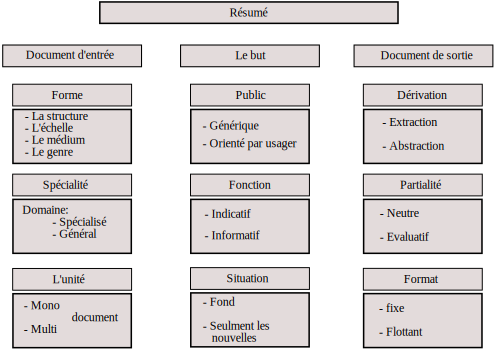
\includegraphics{RA/classif-resume.pdf} % % %[width=140mm]
 \caption{Les différentes classes d'un résumé automatique.}
 \label{fig:classif-resume}
\end{center}
\end{figure}

\subsection{Le document d'entrée}

Les documents utilisés comme entrée d'un système de résumé automatique, peuvent prendre plusieurs formes. 
Ils peuvent aussi être spécialisés pour un domaine, comme ils peuvent appartenir à des domaines arbitraires. 
Si ces documents ont le même thème, on peut les prendre tous comme entrée, alors un système de résumé peut être mono-document ou multi-document. 
Donc, on peut déduire qu'il existe trois façons de classifier le résumé en fonction du document d'entrée: selon sa forme, selon sa spécialité, et selon l'unité.

\subsubsection{La forme}

La forme contient plusieurs aspects: la structure, l'échelle, le médium, et le genre. 
La structure comprend l'organisation explicite comme le marquage par des entêtes (exp. l'objectif, data, méthode, etc.), 
et aussi la structure introduite dans le document comme les modèles rhétoriques familiers (exp. une déclaration suivi d'une élaboration). 
Il est plus approprié ou non de préserver la structure de document dans le résumé. 
En prenant les articles scientifiques comme un exemple, la structure commune dans ce type de document contient les composants: l'introduction, les travaux reliés, le travail réalisé, l'évaluation, et la conclusion. 
Si on ne veut pas préserver la structure de ce document, on peut simplement faire un résumé sur son contenu entier. 
Sinon, le résumé va avoir comme contenu, le résumé de chaque composant du document d'entrée. 
Le travail de \cite{93-paice-jones} est un exemple des travaux qui prennent en considération la structure du document. 
Il utilise comme documents d'entrée, les papiers de recherche très structurées en examinant un corpus des articles pour en extraire les différents patterns des structures existantes. 
Il y a aussi le travail de \cite{04-farzindar-al}, qui traite les textes juridiques en se basant sur leur structure qui comporte quatre thèmes: INTRODUCTION, CONTEXTE, RAISONNEMENT JURIDIQUE et CONCLUSION. 

Du fait qu'on peut résumer un paragraphe comme on peut résumer un livre, l'échelle est importante puisqu'elle contient l'implication pas seulement pour le degré de réduction de résumé, mais aussi pour l'ampleur possible de la transformation du contenu. 
Ainsi, un roman très long peut être aperçu et présenté dans un résumé plus qu'un petit article de nouvelles. 
Un des exemples sur la petite échelle est le travail de \cite{06-kazantseva} dont l'objectif était de résumer les histoires courtes afin d'aider le lecteur à déterminer s'il est intéressé ou non par l'histoire, en fournissant une idée sur les paramètres de cette histoire (comme les caractères, heure, lieu, etc.) sans donner de détails.

Le médium est le support du document d'entrée. 
En regardant aux recherches sur le résumé automatique, on trouve que le support le plus utilisé est le texte, bien qu'il existe d'autres supports comme l'image, le son, la vidéo, etc. 
Ces supports contiennent des informations qu'on peut extraire et résumer de même principe que celui du document texte. 
Parmi les travaux qui concernent le résumé d'un document non textuelle, on peut citer: le résumé des enregistrements audio \cite{01-hori-furui} et \cite{04-Inoue-al}, résumé des vidéos comme dans \cite{03-ekin-al} et \cite{06-albanese-al} qui ont comme but de résumer des vidéo concernant le football, ou des images comme dans le travail de \cite{02-carson-al} et \cite{03-feifei-al}.

%Les genres typiques d'une entrée sont les articles de journaux, les pièces d'opinion, les romans, les histoires, les livres, les rapports, etc. 
Différentes techniques de résumés peuvent être appliquées sur différents genres selon différents échelles, et pas sur d'autres. 
Ces genres peuvent âtre des articles de journaux, des pièces d'opinion, des romans, des histoires, des livres, des rapports, etc. 
%Le travail de \cite{06-kazantseva} est un exemple sur un genre spécifique sur l'entrée; il prend comme entrée, les histoires courtes. 
Un exemple est celui de \cite{09-zhan-al} qui prend comme entrée les documents de genre pièces d'opinion (en Anglais: \textit{reviews}).

\subsubsection{La spécialité}

%Selon la spécialité du résumé par rapport aux documents utilisés, on peut considérer le résumé automatique comme étant de type domaine spécialisé ou générale. 
Le résumé automatique peut être général ou spécifique à un domaine précis. 
Lorsque les documents d'entrée ont tous le même domaine, il est plus approprié d'utiliser un système de résumé automatique spécialisé pour ce domaine. 
Donc, ce type de résumé peut diminuer le degré d'ambiguïté des termes, les mots particuliers et usage de grammaire, et le formatage spécialisé.
%Ceci le rendre plus approprié pour les résumés par abstraction (génération) \cite{93-mitkov}.
Un des exemples sur un résumé de domaine spécifique est le travail de \cite{07-reeve-al} qui s'intéresse aux textes biomédicaux pour aider les médecins à lire les informations concernant les tests cliniques des patients. 
Dans le domaine de droit, on peut citer le travail de \cite{04-farzindar-al}, qui prend en entrée des textes juridiques afin de permettre aux juristes de consulter rapidement les idées clés d'une décision juridique et trouver les jurisprudences pertinentes à leurs besoins.

D'autre part, un résumé de domaine général est dérivé d'un ou plusieurs documents d'entrée dans n'importe quel domaine. 
Un exemple de résumé de domaine générale est donné par le travail de \cite{03-nomoto-matsumoto} qui peut être appliqué pour n'importe quelle domaine, en exploitant la diversité des concepts dans le document d'entrée.

\subsubsection{L'unité}

Selon le nombre de sources, on peut classifier le résumé automatique de documents en deux catégories: Mono-document et multi-documents. 
Un résumé mono-document est un résumé qui traite un seul document en entrée (même si le processus utilise des données compilées antérieurement d'autres documents). 
Il existe plusieurs recherches sur le résumé automatique mono-document, commençant par le travail de Luhn \cite{58-luhn}. 
Parmi ces travaux, on peut prendre comme exemple: \cite{69-edmundson}, \cite{93-mitkov}, \cite{95-kupiec-al}, \cite{98-hovy-lin}, \cite{04-farzindar-al}, etc.

D'autre part, un résumé multi-documents est un résumé qui couvre le contenu de plusieurs documents en entrée, et qu'il est utilisé seulement si ces documents sont reliés par un même thème. 
Il parait que ce type de résumé a été utilisé pour la première fois par \cite{95-mckeown-radev}, en développant le système SUMMONS\footnote{SUMMONS: SUMMarizing Online NewS articles}. %\cite{07-das-martins}. 
Un exemple sur le résumé multi-documents est le travail de \cite{09-boudin-torresmoreno} qui se considère comme le premier travail qui contient une évaluation d'une approche de résumé automatique multi-documents sur les textes en français. 

\subsection{Le but}

Un système de résumé peut être générique où le résumé toujours procède de la même façon quelque-soit l'utilisateur, ou il peut être contrôlé par l'utilisateur. 
Il peut être destiné pour indiquer seulement une idée sur le document sans donner aucun contenu, comme il peut être destiné pour informer l'utilisateur sur le contenu du document, en fournissant une version courte.
Il peut fournir un résumé détaillé en supposant que l'utilisateur n'a aucune connaissance préalable du thème, ou juste fournir les nouvelles.
Donc, selon le but de résumé, on obtient trois facteurs de classification : le public, la fonction, et la situation. 
% Ils sont les facteurs les plus importants selon \cite{99-sparckjones}, puisqu'ils sont critiques, leurs implications peuvent s'étendre, et ils sont la base d'évaluation.

\subsubsection{Le public}

Selon le public, on peut classifier le résumé sur deux catégories: générique et orienté par requête (profil utilisé). 
Un résumé générique est un résumé qui fournit le point de vu de l'auteur (les auteurs) sur un ou plusieurs documents d'entrée, en donnant la même importance pour tous les thèmes majeurs. 
Autrement dit, il ne tient pas compte de ce que l'utilisateur veut chercher. 
Il existe plusieurs exemples sur ce type de résumé, parmi eux on trouve \cite{06-kazantseva}.
%\cite{05-usunier-al} donne une méthode statistique pour le résumé automatique à base d'apprentissage qui extraie les phrases pertinentes d'un document. 
%Ce choix n'implique pas qu'on ne peut pas utiliser la requête d'utilisateur dans sa méthode.
Le but dans ce travail est de fournir au lecteur un bref résumé sur une histoire donnée. 
L'utilisateur dans ce travail est supposé chercher sur le thème général de l'histoire, pour juger s'il veut la lire ou non. 
Si on utilise un résumé orienté par requête, donc l'utilisateur doit savoir préalablement ce qu'il cherche, et le but devient absurde. 
%Donc, on peut conclure qu'il existe des travaux dont le but ne nous permet pas d'utiliser un résumé orienté par requête.

Un résumé orienté par requête (ou orienté utilisateur) préfère des thèmes spécifiques ou aspect(s) de document, en répondant sur les envies des utilisateurs pour chercher seulement sur ces thèmes en particulier. 
Il peut être explicite, en sélectionnant les thèmes pertinents. 
Comme il peut être implicite, en négligeant les thèmes qui ne sont pas en relation avec les intérêts de l'utilisateur. 
%Un exemple sur le résumé dirigé par une requête est le travail par \cite{05-usunier-al} qui est un système de résumé automatique couplé à un moteur de recherche, pour permettre aux utilisateurs d'évaluer rapidement la pertinence réelle d'un document par rapport à leur requête. 
Le travail de \cite{09-liu-al} contient une sorte de résumé par requête, lorsque l'utilisateur sélectionne un mot-clé un résumé s'affiche suivant le thème concernant ce mot-clé.

\subsubsection{La fonction}

Selon la fonction, le résumé peut être indicatif ou informatif. 
Le résumé indicatif fournit seulement une indication sur la matière du sujet principal ou le domaine de document(s) d'entrée sans introduire son contenu. 
D'après \cite{04-crispino-couto}, "\textit{un résumé indicatif peut être considéré comme une aide à l'utilisateur pour juger la pertinence du document et l'intérêt qu'il pourrait y avoir à lire le texte original}".
La recherche des mots-clés et thème d'un document est considérée comme une sorte de résumé indicatif, le travail de \cite{09-liu-al} en est un exemple. 
Ce travail est destiné pour aider les utilisateurs à analyser une grande quantité de textes, en fournissant les mots-clés et les thèmes, présentés d'une manière graphique et distribués au long du temps. 
Leur système a été appelé par TIARA\footnote{TIARA: Text Insight via Automated, Responsive Analysis}, une illustration sur la présentation graphique est donnée dans la figure \ref{fig:tiara}.
\begin{figure}[ht]
\begin{center}
\includegraphics[width=140mm]{RA/tiara.pdf} % % %[width=140mm]
 \caption[Un résumé de 10,000 emails dans l'année 2008, créé par TIARA]{Un résumé de 10,000 emails dans l'année 2008, créé par TIARA \cite{09-liu-al}.}
 \label{fig:tiara}
\end{center}
\end{figure}

Un résumé informatif reflet le contenu (ou une partie), et nous permet de décrire le contenu du document d'entrée. 
D'après \cite{04-crispino-couto}, "\textit{Un résumé informatif fournit une information sur tous les points importants du document en cherchant à couvrir tous les sujets traités par le document}".
Ainsi, après la lecture d'un résumé informatif, on peut expliquer sur quel sujet le document d'entrée peut-être, mais pas nécessairement qu'est-ce qu'il peut contenir. 
Deux exemples sur le résumé informatif sont: \cite{09-boudin-torresmoreno} pour le résumé multi-documents et \cite{05-usunier-al} pour le résumé mono-document.

\subsubsection{La situation}

Le résumé selon la situation peut être un résumé de fond (\textit{background}) ou un résumé qui rapporte Seulement-les-nouvelles. 
Un résumé de fond suppose que la connaissance antérieure de lecteur sur le cadre général du contenu de document(s) d'entrée est très pauvre, et donc il inclut des matériels d'explication, comme la situation des places, le temps, et les acteurs. 
Le travail de \cite{06-kazantseva} peut être considéré comme un résumé automatique de fond, puisqu'il assume l'absence de connaissance préalable du lecteur sur le document d'entrée, et donne des informations sur le temps, les places, les caractères, etc.

Un résumé de type Seulement-les-nouvelles contient seulement les thèmes nouveaux ou principaux, en supposant que le lecteur a un fond suffisant pour les interpréter dans le contexte.
% il peut s'appliquer sur le multi-documents surtout. 
Le travail de \cite{10-bysani} présente un système de résumé automatique qui détecte les nouveau thèmes après une période de temps. 
Il est considéré comme un système de résumé multi-documents; qui détecte la nouveauté dans un document par rapport aux documents passés.

\subsection{Le document de sortie}

Le résumé d'un document peut être obtenu de deux manières: la première est de prendre les phrases (ou des parties) qu'elles semblent plus probable de représenter ce document, la deuxième est de générer le résumé. 
Il peut refléter le document d'entrée sans introduire des jugements, comme il peut porter des jugements sur son contenu.
Tandis que le format du résumé peut être fixe pour tous les documents d'entrée, comme il peut varier selon les types de ces documents.
Les trois critères de classification, en observant le document de sortie, sont: la dérivation, la partialité, et le format.

\subsubsection{Dérivation}

De ce point de vu, un résumé est soit une extraction ou une abstraction. 
Une extraction est une collection de passages (des mots jusqu'à des paragraphes) extraite d'un document d'entrée et produite textuellement comme un résumé. 
Les premières techniques d'extraction ont utilisé le calcul de score pour chaque phrase en fonction des critères tels que la fréquence de mots de phrase \cite{58-luhn}, la position dans le texte \cite{58-baxendale,69-edmundson}, les phrases clés \cite{69-edmundson}. 
Des méthodes d'extraction récentes utilisent d'autres techniques plus sophistiquées pour décider quelle phrase va être extraite. 
Ces techniques dépendent souvent sur l'apprentissage automatique pour identifier les critères importants, sur l'analyse du langage naturel pour identifier les passages clés, ou sur les relations entre les mots plutôt que des sacs de mots \cite{02-radev-al}.

Une abstraction est un texte (document en général) nouvellement généré, produit de certaines représentations internes, et qui est un résultat de l'analyse de l'entrée. 
Le résumé par abstraction est difficile à concevoir, en le comparant avec le résumé par extraction, mais on peut le rendre moins difficile en utilisant quelques techniques. 
Parmi ces techniques, la conception d'une méthode de résumé destinée à un domaine spécifique des documents, cela rend le processus plus facile, comme il est indiqué par \cite{93-mitkov}. 
Pour éviter le problème de différenciation entre les concepts importants dans le texte entre autres, l'auteur utilise un domaine spécifique pour les documents d'entrée.

\subsubsection{Partialité}

Ce critère est principalement appliqué quand le matériel d'entrée est un sujet d'opinion ou pré-jugement. 
Un résumé selon la partialité peut être neutre ou évaluatif. 
Un résumé neutre reflète le contenu de document(s) d'entrée, soit partialement ou impartialement, sans introduire des critiques ou évaluations. 
La plupart des recherches dans le résumé automatique sont de ce type.

Un résumé évaluatif inclut quelques jugements propres au système, soit explicitement (en utilisant des déclarations d'opinion) ou implicitement (en incluant des matériels d'un pré-jugement et l'omission des matériels avec un autre). 
Le travail de \cite{12-workman-al} représente un système de résumé automatique destiné pour les documents médicales, et combiné avec un outil de décision, afin d'aider les médecins dans leurs décisions. 
Un autre exemple est celui présenté dans \cite{09-genereux-bossard} qui traite les textes d'opinion par l'analyse de blogs, où sont exprimées à la fois des informations factuelles et des prises de position sur les faits considérés.

\subsubsection{Le format}

Un résumé, selon le format, peut être fixe ou flottant. 
Un résumé d'un format fixe est créé pour une utilisation, utilisateur (ou classe d'utilisateurs), ou situation spécifique. 
Comme tel, il peut se conformer aux conventions internes appropriées de soulignement, formatage, etc.

Un résumé d'un format flottant est un résumé ayant un format varié; il est créé et affiché avec des préférences variées, pour des différents utilisateurs, et des différents buts. 
Par exemple, pour un utilisateur donné, le système produit un résumé au format d'une table, et pour un autre utilisateur, pour le même document, il affiche un texte.

%========================01========================%
%==================================================%
\section{Étapes du résumé automatique}

Dans le résumé automatique de documents, on peut identifier trois différentes étapes \cite{98-hovy-lin, 99-sparckjones}. 
La plupart des systèmes aujourd'hui utilisent la première étape seulement. 
Ces étapes sont: l'identification du thème, l'interprétation, et la génération du résumé (voir la figure \ref{fig:proc-resume}). 
L'identification des thèmes produit un résumé simple; une fois le système repère les unités importantes, il les présente comme un extrait. 
Ensuite, l'interprétation qui comporte la fusion des concepts, l'évaluation, ou autres procédures qui utilisent une connaissance autre que le (les) document(s) d'entrée. 
Le résultat de l'interprétation est un abstrait non lisible, ou un extrait incohérent. 
Donc, l'étape de génération sert à produire un texte (document) lisible par l'humain, et dans le cas de l'extrait cette étape peut être considérée comme étape de "lissage" pour rendre le résumé plus cohérent.

\begin{figure}[ht]
\begin{center}
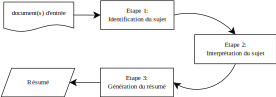
\includegraphics{RA/proc-resume.pdf} % % %[width=140mm]
 \caption{Procédure de résumé automatique.}
 \label{fig:proc-resume}
\end{center}
\end{figure}

\subsection{Étape 1: Identification des thèmes}

Elle sert à produire un résumé simple (extrait) en détectant les unités importantes dans le document (mot, phrase, paragraphes, etc.). 
Les systèmes de résumé qui utilisent seulement l'étape d'identification du thème, produisent un résumé extractif. 
Ceci se fait par filtrage du fichier d'entrée pour obtenir seulement les thèmes les plus importants. 
Une fois ces thèmes identifiés, ils sont présentés sous forme d'un extrait.

Pour effectuer cette étape, presque tous les systèmes utilisent plusieurs modules indépendants. 
Chaque module attribue un score aux unités d'entrée (mot, phrase ou passage plus long), puis un module de combinaison combine les scores pour chaque unité afin d'attribuer un score unique. 
Enfin, le système renvoie les unités du plus haut en score, en fonction de la longueur du résumé, demandé par l'utilisateur ou fixé préalablement par le système.

\subsection{Étape 2: Interprétation des thèmes}

Dans l'interprétation, le but est de faire un compactage en réinterprétant et en fusionnant les thèmes extraits pour avoir des thèmes plus brefs. 
Ceci est indispensable du moment que les abstraits sont généralement plus courts que les extraits équivalents. 
Cette deuxième phase de résumé automatique (passage de l'extrait vers l'abstrait) est naturellement plus complexe que la première. 
Pour compléter cette phase, le système a besoin de connaissances sur le monde (par exemple, les anthologies), puisque sans connaissance aucun système ne peut fusionner les sujets extraits pour produire des sujets moins nombreux afin de former une abstraction. 
Lors de l'interprétation, les thèmes identifiés comme importants sont fusionnés, représentée en des termes nouveaux, et exprimé en utilisant une nouvelle formulation, en utilisant des concepts ou des mots qui n'existent pas dans le document original. 

\subsection{Étape 3: Génération du résumé}

% Introduction à l'étape
Le résultat de l'interprétation est un ensemble de représentations souvent non lisibles, c'est le cas du résumé par abstraction.
Pour le résumé extractif, le résultat est un extrait rarement cohérent, à cause des références coupées, la négligence des liens entre les phrases, et la redondance ou la négligence de quelques matériels. 
De ce fait, les systèmes incluent une étape de génération du résumé afin de produire un texte cohérent et lisible par l'humain. 

% En général: dans le cas de l'abstraction
Dans cette étape, le système a besoin d'utiliser des techniques de la génération de langage naturel qui, selon \cite{98-hovy-lin}, a besoin de deux modules: le micro-planeur et le générateur des phrases. 
Le micro-planeur, dans le contexte du résumé automatique, a comme fonction d'assurer que l'information sélectionnée par les deux étapes précédentes (identification et interprétation du thème) est rédigée d'une manière compacte et brève autant que possible en restant dans un état grammatical. 
Il peut être construit pour mener son travail sur deux niveaux: le niveau textuel et le niveau représentatif. 
Dans le premier niveau, l'entrée est une liste de phrases ou fragments de phrases, et la sortie est une liste compacte de phrases. 
Dans le deuxième niveau, l'entrée est exprimée sous une notation abstraite, et la sortie est une spécification abstraite et syntaxique pour chaque phrase. 
La sortie de ce niveau n'est pas lisible par l'humain c'est pour ça il faut passer par la génération des phrases. 
Un des micro-planeurs destinés pour le résumé automatique est celui de \cite{95-mckeown-radev}.

Le deuxième module est le générateur de phrases, qui transforme une spécification détaillée d'une ou plusieurs unités propositionnelles vers une phrase grammaticalement correct. 
Il existe des générateurs de phrases, qui sont relativement faciles à utiliser, pour les recherches. 
Parmi ces générateurs, il y a Penman \cite{91-hovy}, FUF/SURGE \cite{92-elhadad}, RealPro \cite{97-lavoie-rambow}, et NITROGEN \cite{98-langkilde-knight}. 

Les résumés par extraction n'exigent pas l'étape de génération, mais certaines incohérences vont être observées lorsqu'on extrait des phrases (ou autres unités), et on les assemble en ordre d'importance ou de l'emplacement dans le document. 
Parmi les aspects qui rend le texte incohérent ou non courant, les suivants:
\begin{itemize}
\item La répétition des clauses ou phrases nominales; qui peut être fixée par l'agrégation dans une combinaison.
\item La répétition des entités nommés; qu'on peut fixer en substituant ces entités par des pronoms.
\item L'inclusion des matériels moins importants comme les parenthèses, ceci peut être réglé par la suppression de ces matériels.
\end{itemize}
Dans \cite{99-mani-al2}, les auteurs décrivent un programme de révision du résumé, qui prend en entrée des extraits simples et produit des résumés plus courts et plus lisibles. 
On peut résoudre, aussi, d'autres problèmes d'incohérence qui sont plus difficiles comme les liens anaphoriques cassés, ou les liens entre les phrases et la fluidité du sens. Comme on peut utiliser la compression des phrases afin de rendre le résumé plus court et plus précis.

%========================01========================%
%==================================================%
\section{Approches de résumé automatique}

Il existe deux grandes approches pour le résumé automatique: l'approche statistique et l'approche linguistique. 
L'approche statistique est la plus ancienne, elle revient au années 50 lorsque Luhn a conçu le premier outil du résumé automatique \cite{58-luhn}. 
L'idée d'utiliser l'intelligence artificielle est apparue dans les années 80, pour montrer la capacité de compréhension, c'est ainsi que la méthode linguistique a apparue \cite{02-minel}.

\subsection{L'approche statistique}

L'approche statistique se trouve généralement dans l'étape d'identification de thèmes. 
C'est l'approche la plus ancienne, elle revient au début de recherches sur le résumé automatique dans les années 50. 
Les méthodes statistiques n'utilisent pas de ressources linguistiques, elles sont basées essentiellement sur le calcul d'un score associé à chaque unité (phrase) afin d'estimer son importance dans le texte.

\subsubsection{Le principe}

Le principe de la méthode statistique consiste à sélectionner les unités (phrases) saillantes et les combiner pour avoir un résumé. 
L'approche statistique comprend les trois phases illustrées dans la figure \ref{fig:app-stat}.

\begin{figure}[ht]
\begin{center}
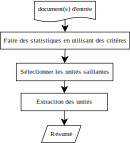
\includegraphics{RA/app-stat.pdf} % % %[width=70mm]
 \caption{Résumé par approche statistique.}
 \label{fig:app-stat}
\end{center}
\end{figure}

La première étape consiste à faire des statistiques sur des critères pour chaque unité (pour un document texte, elle peut être une phrase, un paragraphe, etc.). 
Pour le résumé d'un document texte, ces critères peuvent être: la fréquence des mots, la position des mots, les mots de titre, etc. 
La deuxième phase consiste à sélectionner les unités saillantes dans le texte, en se basant sur les statistiques précédentes, et en attribuant à chaque unité un score selon ces critères. 
Enfin, la phase d'extraction qui consiste à éliminer les unités ayant un score très faible, et donc qui ne sont pas pertinentes dans le document. 
%Cette méthode, ainsi que ses différentes étapes vont être discutés dans le deuxième chapitre.

Le calcul du score de chaque unité se fait en accumulant les poids de chaque critère présent dans cette unité, multiplié par un coefficient spécifique pour ce critère. 
La méthode de calcul du score d'une unité (exp. phrase) $P$ est donnée par l'équation \ref{eq:score-stat}. 
\begin{equation}
\label{eq:score-stat}
Score(P) = \sum_{1 \leq i \leq k} {\alpha_i * C_i(P)}
\end{equation}
Où:
\begin{itemize}
\item $k$ étant le nombre total de critères retenus pour calculer le score de l'unité (exp. phrase);
\item $C_i$ est la fonction calculant la valeur numérique d'un critère $ i $ appliqué à l'unité (exp. phrase);
\item $\alpha_i$ est le coefficient associé au critère $ i $.
\end{itemize}

\subsubsection{Critiques de l'approche statistique}

Les méthodes statistiques sont des méthodes simples, qui attribuent de score en se basant sur certains critères dans le document. 
Il est plus aisé de combiner un ensemble de critères de natures différentes pour exprimer la valeur de pertinence globale d'une phrase (mais aussi d'un paragraphe, etc.).

L'inconvénient majeur de cette méthode est l'incohérence. 
Il existe deux grandes origines de l'incohérence: les anaphores et la structure de phrases. 
Pour les anaphores, on peut trouver dans le résumé un lien anaphorique et qui n'a pas de sens, puisque la phrase qui l'exprime a été éliminée. 
L'autre origine qui est la structure des phrases; lorsqu'on fait l'extraction des phrases, il se peut que les phrases de résumé n'ont aucune relation rhétorique entre elles. 
En plus, on peut trouver dans le résumé des phrases qui sont identiques sémantiquement, et donc un problème de récurrence est vite observé.

%========================01========================%
%==================================================%
\subsection{L'approche linguistique}

%TODO contraduction ??? non pas de contraduction
%pas de contaduction puisque l'approche linguistique peut être extactive comme elle peut être abstractive
L'approche linguistique exploite le savoir linguistique pour générer le résumé, soit par extraction ou par abstraction. 
Elle se passe dans les trois étapes de résumé automatique, précédemment parlé. 
Plusieurs théories entrent dans le cadre de cette approche à savoir : la Théorie de la Structure Rhétorique, et les chaînes lexicales. 
Pour un document (ou plusieurs) d'entrée, le système utilise les informations linguistiques pour créer une représentation de l'entrée. 
Ensuite, cette représentation va être réduite en utilisant des règles de réduction, soit en gardant les phases les plus importantes ou en créant une nouvelle représentation. 
Enfin, l'étape de génération du résumé, qui sert à fusionner les phrases extraites pour avoir un résumé extractif, ou transformer la représentation réduite à un résumé par abstraction. 
La figure \ref{fig:app-ling} illustre les différentes étapes suivies dans l'approche linguistique.
\begin{figure}[ht]
\begin{center}
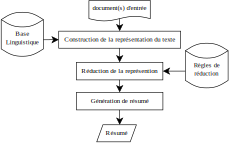
\includegraphics{RA/app-ling.pdf} % % %[width=140mm]
 \caption{Un modèle général pour l'approche linguistique de résumé automatique.}
 \label{fig:app-ling}
\end{center}
\end{figure}

\subsubsection{Les chaînes lexicales}

Dans \cite{97-barzilay-elhadad}, les auteurs ont conduit un travail qui utilise une quantité considérable d'analyse linguistique. 
Ils ont utilisé une méthode qui s'appelle: "chaîne lexicale" (\textit{lexical chain}); définit par une séquence des mots reliés dans un texte, avoir une distance courte (les mots adjacents ou phrases), ou distance longue (le texte entier). 
La production du résumé passe par les étapes suivantes: segmentation du texte, identifications des chaînes lexicales, et l'utilisation des chaînes lexicales puissantes pour identifier les phrases saillantes. 
Ils ont essayé d'atteindre une base entre \cite{95-mckeown-radev} qui effectue une analyse profonde de la structure sémantique du texte, et \cite{58-luhn} qui utilise des statistiques sur les mots du document. 
Les auteurs modélisent la notion de cohésion dans le texte comme une moyenne d'assembler les différentes parties du texte. 
La cohésion lexicale est un exemple où les mots reliés sémantiquement sont utilisés, la phrase suivante illustre cette notion:
\begin{center}
\textit{John a acheté une Peugeot. Il aime les voitures.}
\end{center}
Ici, le mot "voiture" réfère au mot "Peugeot" dans la phrase qui précède, et donne un exemple sur la cohésion lexicale. 
Le phénomène de cohésion ne se passe pas seulement au niveau du mot, mais aussi au niveau des séquences de mots, qui donne des chaînes lexicales. 
Les mots sémantiquement reliés ainsi que les séquences des mots, sont identifiés dans le document, et plusieurs chaînes sont extraites, formant une représentation du document. 
Pour trouver les chaînes lexicales, les auteurs ont utilisé Wordnet \cite{95-miller}, en suivant trois étapes:
\begin{enumerate}
\item Sélection d'un ensemble des mots candidats.
\item Pour chaque mot candidat, trouver la chaîne appropriée en se basant sur un critère de lien entre les membres de la chaîne.
\item S'il existe une chaîne, insérer le mot dans la chaîne et mettre à jour en conséquence.
\end{enumerate}

Le lien est mesuré par la distance dans Wordnet. 
Les noms simples et les noms composés sont utilisés comme point de départ pour trouver l'ensemble des mots candidats dans l'étape 1. 
Enfin, les chaînes lexicales les plus fortes sont utilisées pour créer le résumé. 
Les scores de ces chaînes sont calculés en se basant sur leurs longueurs et homogénéités. 
Puis, les auteurs utilisent quelques heuristiques pour sélectionner les phrases signifiantes. 

\subsubsection{La structure rhétorique}

Dans \cite{94-ono}, les auteurs introduisent un système de génération automatique de résumé pour les discours japonais. 
Ils ont élaboré une procédure pratique pour extraire la structure rhétorique du discours: un arbre binaire représentant les relations entre les parties de la phrase. 
Cette structure a été extraite en utilisant une série d'étapes basées sur le TALN: analyse des phrases, extraction des relations rhétoriques, segmentation, génération de candidat, et jugement de pertinence. 
L'évaluation est basée sur l'importance relative entre les relations rhétoriques.
Dans cette étape, les nœuds de l'arbre représentant la structure rhétorique, sont taillés pour réduire la phrase, en gardant ses parties importantes. 
Le processus est réitéré au niveau des paragraphes afin de produire, finalement, un résumé.
%Evaluation was done with respect to sentence coverage and 30 editorial articles of a Japanese newspaper were used as the dataset. 
%The articles had corresponding sets of key sentences and most important key sentences judged by human subjects. 
%The key sentence coverage was about 51\% and the most important key sentence coverage was 74\%, indicating encouraging results.

\cite{98-marcu} décrit une approche unique pour le résumé automatique qui, au contraire aux autres travaux ultérieurs, ne suppose pas que les phrases dans un document forment une séquence absolue. 
L'auteur utilise les heuristiques basées sur la théorie de structures rhétoriques, combinées avec les critères classiques qui ont été utilisés dans la littérature de résumé automatique. 
Cette théorie repose sur deux concepts: le noyau et le satellite. 
%La théorie du discours utilisée dans cet article est la théorie de structure rhétorique, qui se tient entre deux pièces non superposées de texte: le noyau et le satellite. 
La distinction entre le noyau et le satellite vient de l'observation empirique que le noyau exprime ce qu'il est plus essentiel pour l'objectif de l'auteur que le satellite. 
En plus, le noyau d'une relation rhétorique est compréhensible indépendamment du satellite, mais pas vice versa. 
La figure \ref{fig:arbre-rhet} illustre les relations rhétoriques entre les différentes phrases d'un texte. 
Les chiffres représentent les emplacements des phrases dans le texte, les nœuds pointillés représentent les satellites et les nœuds normaux représentent les noyaux.
\begin{figure}[ht]
\begin{center}
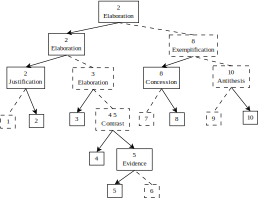
\includegraphics{RA/arbre-rhet.pdf} % % %[width=140mm]
 \caption[Exemple d'une arbre de discours]{Exemple d'une arbre de discours \cite{98-marcu}.}
 \label{fig:arbre-rhet}
\end{center}
\end{figure}

\subsubsection{Critiques de l'approche linguistique}

L'utilisation de cette approche nous garantit une analyse plus profonde du texte d'entrée; on peut examiner les liens sémantiques entre les mots (les synonymes, les antonymes), le sens des phrases, les différents concepts existants et les relations entre eux, etc. 
Un autre point fort de cette approche, est le respect de l'acheminement de l'auteur; on peut extraire les différentes idées existantes dans le texte et générer un résumé qui respecte leur évolution.

Cependant, cette approche reste très lourde, à cause de l'utilisation de traitement de langage naturel qui consomme beaucoup de ressources. 
En plus, les outils de TALN existants ne sont pas assez performants, ainsi l'utilisation de plusieurs outils peut introduire des erreurs de traitement. 
Un autre obstacle pour cette approche est la dépendance du texte d'entrée, donc les méthodes développées par cette approche ne peuvent pas être générales, elles doivent être destinée pour une langue spécifique et/ou un genre déterminé. 

%========================01========================%
%==================================================%
\section{Applications du résumé automatique}

Avec l'augmentation considérable du volume des informations sur Internet, il est devenu très difficile de sélectionner l'information pertinente. 
L'information est publiée simultanément sur plusieurs canaux média avec des versions variantes, par exemple, un journal papier, un journal web, message SMS, des nouvelles de radio, etc. 
La personnalisation de l'information pour les différents canaux et formats est une fonction d'édition immense qui demande notamment de raccourcir le texte original.

Le résumé automatique apporte une solution à ce problème et automatise complètement ce travail. 
En plus, les documents deviennent accessibles par d'autres langues en les résumant premièrement avant traduction, ceci peut être, dans la plupart des cas, suffisant pour juger de la pertinence d'un document avec une langue étrangère. 
De ce fait, on peut éviter le travail de traduction de tout le document manuellement. 
Le résumé automatique peut être utilisé pour résumer un texte avant qu'un synthétiseur de parole automatique le lit, de ce fait on peut réduire le temps nécessaire pour extraire les données clés dans le document. 
En particulier, il peut être utilisé pour préparer l'information pour être utilisée dans les petites appareilles mobiles, comme les PDA, dont le besoin d'une réduction considérable du contenu est nécessaire.

D'après l'institut national américain de normalisation (ANSI): "\textit{Un résumé bien préparé permet aux lecteurs d'identifier le contenu de base d'un document rapidement et avec précision, afin de déterminer sa pertinence pour leurs intérêts, et donc de décider s'ils ont besoin pour lire le document dans son intégralité}" \cite{07-hassel}. 
En effet, le résumé s'avère très bénéfique dans plusieurs tâches d'acquisition d'information, quelques exemples sont donnés dans \cite{75-borko-bernier}:
\begin{itemize}
\item Les résumés permettent d'économiser le temps de lecture;
\item Les résumés facilitent la sélection;
\item Les résumés facilitent les recherches documentaires;
\item Les résumés améliorent l'efficacité d'indexation;
\item Les résumés aident dans la préparation des revues.
\end{itemize}

Parmi les exemples de l'utilisation de résumé, le travail de \cite{07-yang-wang} qui présente un modèle de résumé de documents web pour les appareils portables. 
Le modèle est basé sur la théorie des fractales, il génère un résumé squelette. 
Ensuite, si l'utilisateur veut voir plus de détail, le système génère des niveaux de détails. 
Un autre exemple est celui de \cite{09-zhan-al}, qui se repose sur le résumé des critiques sur les produits. 
Ceci peut aider les sociétés pour développer les modèles conceptuels, la personnalisation, la recommandation des produits, comprendre le client, et, par conséquent, attirer plus de clients.
Dans l'aide à la décision médical, on peut citer le travail de \cite{12-workman-al}, qui utilise un système de résumé automatique pour améliorer la décision médicale. 
Le travail de \cite{11-uzzaman-al} introduit une idée d'illustrer automatiquement les phrases complexes, en utilisant des résumés qui combinent les images, les structures et des textes simples. 

%TODO Done: ccl sur les domaines d'utilisations multiples et variés
Les domaines d'utilisation de résumé automatique sont multiples et variés, ce qui preuve le besoin de développer des outils pour ça. 
Dans la section suivante, nous allons parler sur quelques outils industriels qui aident l'utilisateur à satisfaire les applications citées précédemment.

%========================01========================%
%==================================================%
\section{Outils industriels}

Pour appliquer les domaines d'utilisation précédemment cités, il faut des outils permettant le résumé automatique. 
Il existe plusieurs outils industriels du résumé automatique de documents. 
Certains de ces outils sont commerciaux, d'autres sont gratuits ou open source. 
Nous allons citer quelques exemples sur ses outils destinés pour le résumé automatique de textes.

\subsection{Essential Summarizer} %Pertinence

Essential Summarizer\footnote{Site web: \url{http://www.essential-mining.com}} est un outil de construction de résumés informatifs pour des textes écrits dans différentes langues (Anglais, français, allemand, Italien, etc.) qui se décline en deux versions. 
La première est conçue pour être incorporé dans des Intranets d'entreprise. 
L'autre version est une application de bureautique traditionnelle destinée à l'utilisation personnelle.

Les deux versions sont fondées sur les travaux de recherche de Lehmam \cite{10-lehmam} et s'appuient sur un même noyau informatique programmé en Java, ce qui facilite la portabilité entre les différentes plateformes matérielles. 
Différents formats d'entrée pour les textes sont traités: ASCII, PDF, Word, RTF, et HTML. 

Le programme est développé en se basant sur l'idée que le lecteur va payer plus d'attention à certaines passages du texte puisqu'elles contiennent les informations que lui intéresse. 
Il utilise des techniques linguistiques pour extraire ces informations: 
\begin{itemize}
\item La reconnaissance d'indices sémantiques appelés marqueurs d'extraction sémantique (MLE) afin d'évaluer la pertinence des phrases isolées et des paragraphes entiers;
\item La spécialisation par domaine, afin de mieux cibler le résumé;
\item La prise en considération des expressions ou des concepts qui sont importants pour les besoins de l'utilisateur;
\item Observation de résumés manuels de textes représentatifs, et analyse de retour d'information (feedback) des utilisateurs.
\end{itemize}
Les  connaissances linguistiques sont stockées dans la base des marqueurs linguistiques d'extraction (MLE) – différentes pour chacune des langues traitées – qui sont des expressions linguistiques auxquelles sont affectées des valeurs. 
La base globale des MLE se décompose au niveaux suivants (voir la figure \ref{fig:lehmam-ling}):
\begin{itemize}
\item Marqueurs linguistiques d'extraction indépendants de tout domaine (MLE généraux);
\item MLE propres à un domaine (médicale, financier, etc.);
\item La terminologie propre au domaine;
\item Mots ou expressions utilisateur;
\item Mots ou expressions d'exclusion.
\end{itemize}

\begin{figure}[ht]
\begin{center}
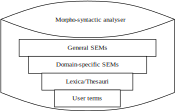
\includegraphics{RA/lehmam-ling.pdf} % % %[width=80mm]
 \caption[Organisation de marqueurs linguistiques]{Organisation de marqueurs linguistiques \cite{10-lehmam}.}
 \label{fig:lehmam-ling}
\end{center}
\end{figure}

L'objectif du système est de repérer les marqueurs de la base des MLE dans le texte à résumer afin de pondérer l'ensemble des phrases du texte. 
Chaque phrase se voit associer un poids qui est la somme des poids des marqueurs linguistiques qu'elle contient. 
Les phrases dont le poids est nul ou très faible sont alors éliminées. 
L'utilisation de lexiques terminologiques spécialisés d'un domaine donnée peut améliorer la pertinence du résumé automatique en termes de son thème. 

\subsection{Summarist}

Summarist\footnote{Site web: \url{http://nlg.isi.edu/research/projects/SUMMARIST.php}} est un système développé par \textit{Information Sciences Institute (ISI)} qui combine l'identification de concepts à l'aide de ressources linguistiques (WordNet, dictionnaires, etc.) avec des techniques issues de l'informatique documentaire. 
Des dictionnaires japonais, espagnol et d'arabe permettent de traiter des textes dans ces différentes langues. 
Le calcul de la pertinence d'une phrase est effectué à l'aide de différents paramètres tels que tf, tf*idf, cue-phrase, etc. 
La pondération de ces paramètres peut être modifiée par l'utilisateur à l'aide d'une interface spécifique.

Le résumé est affiché sous la forme de phrases soulignées en vert dans le texte source accompagné d'informations complémentaires comme la liste des termes proportionnelles à la taille de la phrase et la couleur est un indicateur de l'importance de la phrase, jaune pour signaler l'importance, rouge pour l'inverse.

\subsection{AutoSummarize de Microsoft Office}

Le logiciel Office de Microsoft offre une option de génération automatique de résumés. 
Le résumé est produit par l'extraction de phrases. 
Le système analyse le document et assigne une valeur à chaque phrase, selon certains critères. 
Puis il choisit les phrases qui ont le score le plus haut. 
L'utilisateur peut choisir le taux de réduction et la forme de visualisation du résumé, qui peut être:
\begin{itemize}
\item Souligner les phrases choisies dans le document;
\item Insérer le résumé au début du document;
\item Créer un nouveau document avec le résumé;
\item Afficher uniquement les phrases choisies.
\end{itemize}

\subsection{Copernic}

Copernic summarizer\footnote{Site web: \url{http://www.copernic.com/fr/products/summarizer/}}  est un système de résumé qui utilise des algorithmes basés sur des calculs statistiques et des données linguistiques. 
Il identifie les concepts clés d'un texte et en extrait les phrases les plus marquantes. 
Il supporte plusieurs formats des fichiers, comme les fichiers TXT, Word, PDF, etc. comme il peut résumer les pages web en lui donnant leurs liens. 
Résumé possible de documents en anglais, français, allemand et espagnol.

Grâce à la technologie en instance de brevet WebEssence, laquelle permet d'éliminer le contenu non pertinent des pages Web (dont les publicités et les items de navigation), Copernic Summarizer utilise l'essentiel de cette page web. 

\subsection{Intellexer summarizer}

Intellexer summarizer\footnote{Site web: \url{http://summarizer.intellexer.com/}} est un système de résumé automatique de textes, qui utilise l'approche linguistique pour produire ses résumés. 
En plus du résumé, Intellexer summarizer possède l'option de reconnaître les entités nommées comme les noms des organisations, les noms des personnes. 
Il peut aussi détecter les locations, les positions de personnes, leurs âges et nationalités, les dates, et les périodes. 
Il donne la possibilité de réarranger le résumé en se basant sur les entités sélectionnées. 
Il est considéré comme un système de résumé adaptatif \cite{10-yatsko-al}, qui exécute des algorithmes optimisés pour des genres comme les brevets, textes scientifiques, politiques, économiques, etc. 
Le système est distribué sur une base commerciale; il n'y a aucune information comment ces genres sont sélectionnés. 

\subsection{UNIS summarizer}

UNIS\footnote{UNIS: UNIversal Summarizer} \cite{10-yatsko-al}, est un système destiné pour supporter le résumé adaptatif de textes, qui est le même but que Intellexer summarizer, mais au contraire à Intellexer, ce système est distribué gratuitement. 
Ce système se base sur l'extraction de résumé en appliquant certains paramètres qui sont utilisés pour calculer l'importance d'une phrase. 
Pour chaque genre, des recherches sont conduits pour sélectionner les paramètres les plus probables en utilisant un corpus. 
Pour pondérer les paramètres selon le genre, les auteurs ont suivi les étapes suivantes: 
\begin{enumerate}
\item Ils ont utilisé un algorithme de groupement (clustering) pour normaliser les éléments hétérogènes et grouper le corpus utilisé. 
\item Les paramètres sont pondérés en se basant sur le réseau de neurone, pour déterminer les paramètres adaptés pour les textes artistiques, non artistiques, scientifiques, et journaux.
\item un système de reconnaissance de genre a été développé.
\end{enumerate}
Pour chaque genre, les auteurs ont utilisé 45 paramètres de type statistique, lexical, syntaxique, de position, et discursive.

Le texte d'entrée passe premièrement par un module de traitement préliminaire, qui effectue une analyse lexicale et syntaxique, une analyse morphologique, et une annotation par tags sémantiques ou part of speech. 
Le traitement préliminaire donne un modèle d'objet qui reflète les caractéristiques linguistiques du texte d'entrée. 
Ces caractéristiques ensemble avec les coefficients assignés à l'étape suivante, constituant les paramètres du texte. 
Les paramètres dont le poids est plus grand, sont comparés avec ceux dans la base linguistique contenant le modèle construit avec le corpus. 
Le genre du texte es déterminé en se basant sur le degré de correspondance entre ces paramètres. 
Après la sélection du genre, un algorithme optimisé pour ce genre est appliqué pour avoir le résumé. 
La figure \ref{fig:unis-model} illustre le modèle général du système UNIS. 

\begin{figure}[ht]
\begin{center}
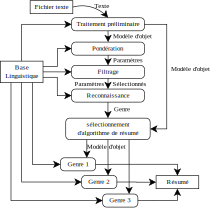
\includegraphics{RA/unis-model.pdf} %[width=140mm]
\caption[Le modèle général de UNIS]{Le modèle général de UNIS \cite{10-yatsko-al}.}
\label{fig:unis-model}
\end{center}
\end{figure}

%TODO done-ccl sur les outils industriels
Le résumé automatique est une nécessite ces jours à cause de bénéfices et des applications qu'on peut avoir en l'utilisant. 
Les outils que nous avons cités parmi autres, sont des outils très utiles qui visent fournir l'utilisateur par des résumés satisfaisantes en se basant sur les technologies que nous avons vu dans ce chapitre. 
Ces outils gratuits ou commercialisés peuvent être d'une grande utilité pour l'utilisateur.

%========================01========================%
%==================================================%
\section{Conclusion}

Dans ce chapitre, nous avons présenté un état de l'art sur le résumé automatique. 
Dans un premier temps, nous avons présenté quelques définitions pour le résumé, afin de comprendre ce domaine. 
Un résumé automatique peut appartient à plusieurs classes ou types, puisque il existe plusieurs critères de classification. 
Donc, nous avons vu qu'on peut diviser ces critères selon le document d'entrée, le but, et le document de sortie. 
Nous avons conclu que le choix de la classe du résumé pour chaque critère peut affecter la méthode de résumé utilisée. 
Ainsi, il est important de spécifier les différentes classes de notre résumé avant de le développer. 
Pour comprendre la fonction de résumé d'une manière générale, sans introduire les différents types et approches existants, nous avons vu que le résumé a trois étapes fondamentales: l'identification des sujets, l'interprétation des sujets, et la génération de résumé. 
Ensuite, nous avons présenté les deux méthodes: statistiques; qui calcule l'importance des unités de document en se basant sur des statistiques menées sur des critères comme la fréquence des mots, etc., et la méthode linguistique qui utilise des méthodes plus profondes pour analyser le document d'entrée et obtenir une représentation de ce document qui va être utilisée pour générer le résumé. 
Nous avons présenté quelques applications de résumé automatique. 
%Le but principal de résumé automatique est d'aider les individus là où ils sont besoin de comprendre le contenu d'un document long, donc il existe des outils industriels qu'on peut utiliser. 
%Nous avons présenté quelques exemples de ces outils, soit commerciaux ou gratuits. 
Enfin, Nous avons présenté quelques outils industriels.

Le domaine de résumé automatique est très vaste, nous avons essayé de couvrir l'essentiel. 
%Le résumé automatique de textes est le plus remarquable parmi les types de résumé automatique, en se basant sur le médium. 
En analysant les deux approches statistique et linguistique, on peut dire que l'approche linguistique est très prometteuse, à ce stade, il n'existe pas encore d'outils TALN puissants et performants. 
Cependant, l'approche statistique n'exige pas de ressources et donne des résultats satisfaisants. 
Malgré sa faible qualité linguistique, l'approche statistique reste une approche très puissante, qui a prouvé son utilité, et spécialement pour les documents scientifiques qui, d'après \cite{58-luhn}, n'utilisent pas une langue complexe et les mots importants sont souvent répétés. 
%Dans le chapitre suivant
Dans le chapitre suivant, nous allons présenter l'approche statistique pour le résumé automatique de texte. 

%========================Le pied de chapitre=======================================
%==================================================================================
\ifx\wholebook\relax\else
 \clearpage
 \let\wholebook=\relax
 \appendix
 \appendixfile{acronyms.tex}
 \bibliographystyle{../use/ESIbib}
 \bibliography{../bib/RA}
 \end{document}
\fi
%==================================================================================

\clearpage

%==================================================================================
%==================================================================================
% Document		:		Chapitre: Approche statistique pour le résumé automatique de textes
%
% Auteur		: 		Abdelkrime ARIES
% Encadreur		:		Dr. Omar NOUALI
% Co-encadreur	:		Mme. Houda OUFAIDA
% Établissement	:		ESI (Ecole Nationale Supérieure d'Informatique; ex. INI) 
% Adresse		:		Oued Smar, Alger, Algérie 
% Année			:		2012/2013
% Grade			:		Magister
% Discipline 	:		Informatique 
% Spécialité	:		IRM (Informatique Répartie et Mobile)
% Titre			:		Résumé automatique de textes
%
%==================================================================================
%==================================================================================

%==========================L'entete de chapitre====================================
%==================================================================================
 \ifx\wholebook\relax\else
  	\documentclass[a4paper,12pt,oneside]{../use/ESIthesis}
  	
  	\usepackage{amsmath,amssymb}             % AMS Math
\usepackage[utf8]{inputenc}
%\usepackage[T1]{fontenc} %,LAE 
\usepackage[T1]{fontenc}
%\usepackage[french,english]{babel}
\usepackage[frenchb]{babel}
\usepackage{microtype}

%\usepackage[left=2.5cm,right=2.5cm,top=2.5cm,bottom=2.5cm,includefoot,includehead,headheight=13.6pt]{geometry}
\usepackage[left=2.8cm,right=2.2cm,top=2.8cm,bottom=2.8cm,includefoot,includehead,headheight=13.6pt]{geometry}
%\usepackage[left=3.8cm,right=3.2cm,top=2.8cm,bottom=2.8cm,includefoot,includehead,headheight=13.6pt]{geometry}
%\usepackage[left=1.5in,right=1.3in,top=1.1in,bottom=1.1in,includefoot,includehead,headheight=13.6pt]{geometry}
\renewcommand{\baselinestretch}{1.5}

% Table of contents for each chapter

\usepackage[nottoc, notlof, notlot]{tocbibind}
\usepackage[french]{minitoc}
\setcounter{minitocdepth}{1}
\mtcindent=15pt
% Use \minitoc where to put a table of contents

\usepackage{aecompl}

% Glossary / list of abbreviations

\usepackage[intoc]{nomencl}
%\renewcommand{\nomname}{List of Abbreviations}

\makenomenclature

% My pdf code

\usepackage[pdftex]{graphicx}
\usepackage[a4paper,pagebackref,hyperindex=true]{hyperref}

%I added
%\usepackage{tabulary}
%\usepackage{longtable}
%\usepackage[table]{xcolor}
\usepackage{indentfirst}


% Links in pdf
\usepackage{color}
%\definecolor{linkcol}{rgb}{0,0,0.4} 
%\definecolor{citecol}{rgb}{0.5,0,0} 

% Change this to change the informations included in the pdf file

% See hyperref documentation for information on those parameters

\hypersetup
{
%bookmarksopen=true,
pdftitle=Résumé Automatique de Textes,
pdfauthor=Abdelkrime ARIES, 
pdfsubject= {Résumé automatique de textes en utilisant une approche statistique, le regroupement, et la classification} , %subject of the document
%%pdftoolbar=false, % toolbar hidden
%pdfmenubar=true, %menubar shown
%pdfhighlight=/O, %effect of clicking on a link
colorlinks=false, %couleurs sur les liens hypertextes
%pdfpagemode=None, %aucun mode de page
%pdfpagelayout=SinglePage, %ouverture en simple page
%pdffitwindow=true, %pages ouvertes entierement dans toute la fenetre
%linkcolor=linkcol, %couleur des liens hypertextes internes
%citecolor=citecol, %couleur des liens pour les citations
%urlcolor=linkcol %couleur des liens pour les url
}



% Some useful commands and shortcut for maths:  partial derivative and stuff

\newcommand{\pd}[2]{\frac{\partial #1}{\partial #2}}
\def\abs{\operatorname{abs}}
\def\argmax{\operatornamewithlimits{arg\,max}}
\def\argmin{\operatornamewithlimits{arg\,min}}
\def\diag{\operatorname{Diag}}
\newcommand{\eqRef}[1]{(\ref{#1})}

\usepackage{rotating}                    % Sideways of figures & tables
%\usepackage{bibunits}
%\usepackage[sectionbib]{chapterbib}          % Cross-reference package (Natural BiB)
%\usepackage{natbib}                  % Put References at the end of each chapter
                                         % Do not put 'sectionbib' option here.
                                         % Sectionbib option in 'natbib' will do.
\usepackage{fancyhdr}                    % Fancy Header and Footer

\usepackage{txfonts}                     % Public Times New Roman text & math font
  
%%% Fancy Header %%%%%%%%%%%%%%%%%%%%%%%%%%%%%%%%%%%%%%%%%%%%%%%%%%%%%%%%%%%%%%%%%%
% Fancy Header Style Options

\pagestyle{fancy}                       % Sets fancy header and footer
\fancyfoot{}                            % Delete current footer settings

%\renewcommand{\chaptermark}[1]{         % Lower Case Chapter marker style
%  \markboth{\chaptername\ \thechapter.\ #1}}{}} %

%\renewcommand{\sectionmark}[1]{         % Lower case Section marker style
%  \markright{\thesection.\ #1}}         %
%\fancyhead[LE,RO]{\bfseries\thepage}    % Page number (boldface) in left on even
%										% pages and right on odd pages
%\fancyhead[RE]{\bfseries\nouppercase{\leftmark}}      % Chapter in the right on even pages
%\fancyhead[LO]{\bfseries\nouppercase{\rightmark}}     % Section in the left on odd pages

\fancyhead[R]{\bfseries\thepage}    % Page number (boldface) in right
\fancyhead[L]{\bfseries\nouppercase{\rightmark}}     % Section in the left on odd pages

\let\headruleORIG\headrule
\renewcommand{\headrule}{\color{black} \headruleORIG}
\renewcommand{\headrulewidth}{1.0pt}
\usepackage{colortbl}
\arrayrulecolor{black}

\fancypagestyle{plain}{
  \fancyhead{}
  \fancyfoot{}
  \renewcommand{\headrulewidth}{0pt}
}

%\usepackage{algorithm}
%\usepackage[noend]{algorithmic}

%%% Clear Header %%%%%%%%%%%%%%%%%%%%%%%%%%%%%%%%%%%%%%%%%%%%%%%%%%%%%%%%%%%%%%%%%%
% Clear Header Style on the Last Empty Odd pages
\makeatletter

\def\cleardoublepage{\clearpage\if@twoside \ifodd\c@page\else%
  \hbox{}%
  \thispagestyle{empty}%              % Empty header styles
  \newpage%
  \if@twocolumn\hbox{}\newpage\fi\fi\fi}

\makeatother
 
%%%%%%%%%%%%%%%%%%%%%%%%%%%%%%%%%%%%%%%%%%%%%%%%%%%%%%%%%%%%%%%%%%%%%%%%%%%%%%% 
% Prints your review date and 'Draft Version' (From Josullvn, CS, CMU)
\newcommand{\reviewtimetoday}[2]{\special{!userdict begin
    /bop-hook{gsave 20 710 translate 45 rotate 0.8 setgray
      /Times-Roman findfont 12 scalefont setfont 0 0   moveto (#1) show
      0 -12 moveto (#2) show grestore}def end}}
% You can turn on or off this option.
% \reviewtimetoday{\today}{Draft Version}
%%%%%%%%%%%%%%%%%%%%%%%%%%%%%%%%%%%%%%%%%%%%%%%%%%%%%%%%%%%%%%%%%%%%%%%%%%%%%%% 

\newenvironment{maxime}[1]
{
\vspace*{0cm}
\hfill
\begin{minipage}{0.5\textwidth}%
%\rule[0.5ex]{\textwidth}{0.1mm}\\%
\hrulefill $\:$ {\bf #1}\\
%\vspace*{-0.25cm}
\it 
}%
{%

\hrulefill
\vspace*{0.5cm}%
\end{minipage}
}

\let\minitocORIG\minitoc
\renewcommand{\minitoc}{\minitocORIG \vspace{1.5em}} %1.5em

\usepackage{multirow}
%\usepackage{slashbox}

\newenvironment{bulletList}%
{ \begin{list}%
	{$\bullet$}%
	{\setlength{\labelwidth}{25pt}%
	 \setlength{\leftmargin}{30pt}%
	 \setlength{\itemsep}{\parsep}}}%
{ \end{list} }

\newtheorem{definition}{Définition }
\renewcommand{\epsilon}{\varepsilon}

% centered page environment

\newenvironment{vcenterpage}
{\newpage\vspace*{\fill}\thispagestyle{empty}\renewcommand{\headrulewidth}{0pt}}
{\vspace*{\fill}}

%%%%%%%%%%%%%%%%%%%%%%%%%%%%%%%%%%%%%%%%%%%%%%%%%%%%%%%%%%%%%%%%%%%%
% Par Karim
%%%%%%%%%%%%%%%%%%%%%%%%%%%%%%%%%%%%%%%%%%%%%%%%%%%%%%%%%%%%%%%%%%%%
%for the degree sign
\usepackage{textcomp} 
\usepackage{bookmark}
\usepackage{framed}
\usepackage{arabtex}
%\usepackage{nashbf}
%\usepackage{atrans}
%calligra font for the remerciement
\usepackage{calligra}

%List of acronyms
\usepackage{acronym}

\newcommand{\racine}{./}

\newcommand{\setracine}[1]{\renewcommand{\racine}{#1}}

\newcommand{\tablefile}[1]{\input{\racine tab/#1}}
\newcommand{\appendixfile}[1]{\input{\racine anx/#1}}
%\newcommand{\chapterfile}[1]{\input{\racine chap/#1}}

\newcommand{\stitle}[1]{
\noindent
\textbf{#1}
}

\newenvironment{itemizeb}
{\begin{list}{\textbullet} {\setlength{\rightmargin}{0cm} \setlength{\leftmargin}{1cm}}}
{\end{list}}


\newenvironment{itemizec}
{\begin{list}{\textopenbullet} {\setlength{\rightmargin}{0cm} \setlength{\leftmargin}{1cm}}}
{\end{list}}


\newcommand{\kexpbox}[1]{

\vspace{5mm}
\noindent
 \fbox{%
   \parbox{0.985\linewidth}{%
   \vspace{2mm}
   {\large  \textbf{Exemple:}}\\
      #1
   }%
 }
}

\newcommand{\kbox}[1]{

\vspace{2mm}
\noindent
 \fbox{%
   \parbox{0.965\linewidth}{%
   \vspace{2mm}
      #1
   }%
 }
}

\newenvironment{kexp}
{
\begin{framed}
\noindent
{\large  \textbf{Exemple:}}\\
}
{
\end{framed}
}

%%%%%%%%%%%%%%%%%%%%%%%%%%%%%%%%%%%%%%%%%%%%%%%%%%%%%%%%%%%%%%%%%%%%
%%%%%%%%%%%%%%%%%%%%%%%%%%%%%%%%%%%%%%%%%%%%%%%%%%%%%%%%%%%%%%%%%%%%

% definitions.
% -------------------

\setcounter{secnumdepth}{3}
\setcounter{tocdepth}{2}

\newcommand{\tab}[1]{{\hskip #1}}
  	 	
  	 	\setracine{../}
  	 	\graphicspath{{.}{../fig/}}
  	 	
  	 	\begin{document}
  	 	
  	 	\dominitoc 
  	 	\selectlanguage {francais}
  	 	%just to create the .toc file, then you can hide it
  	 	%\tableofcontents
  	 	\mainmatter
  \fi
%==================================================================================

\chapter{Approche statistique pour le résumé automatique de textes}
\label{chap:RATstat}
\minitoc

\section{Introduction}

L'approche statistique se caractérise par sa "simple" mise en œuvre, sa robustesse, et son indépendance vis-à-vis le domaine, si on la compare à l'approche linguistique. 
Elle nous apparut très intéressante et prometteuse, étant donné que les outils de recherche de l'information sont en constante évolution. 
L'approche statistique utilise différents critères pour calculer le score de l'unité qu'on veut extraire. 
Ces critères sont combinés de différentes manières afin de procéder à un score qu'on peut utiliser pour juger si l'unité peut être retenue dans le résumé. 
%Avant de calculer le score, il faut d'abord faire un pré-traitement sur le texte d'entrée. 
Ceci nécessite d'effectuer un pré-traitement du texte source.
Les résumés issus de cette approche présentent des inconvénients comme les anaphores, manque de cohérence et cohésion.
Pour diminuer ces limites, une étape de post-traitement est nécessaire. 

Dans ce chapitre, nous allons aborder le travail de Luhn, qui va nous aider à comprendre cette méthode et même les problèmes du résumé automatique. 
Ensuite, comme tout système de RI ou de TALN, ceci nécessite une étape de pré-traitement qui nous garde que l'information pertinente dont le système a besoin. 
Ainsi que les critères fondamentaux pour le calcul du score d'une unité du texte, quelques exemples sur le calcul de score sont ensuite présentés. 
Les scores de ces critères vont être combinées pour avoir un seul score qui nous aide à juger la pertinence d'une unité (en général: phrase), pour ceci nous allons présenter comment peut-on combiner ces différents scores. 
Après, nous allons discuter quelques méthodes utilisées pour améliorer l'approche statistique. 
Enfin, nous allons présenter des méthodes pour améliorer la structure et la lisibilité du résumé résultant, dans la section post-traitement. 
Dans la suite de ce chapitre nous allons utiliser la phrase comme unité d'extraction, à moins qu'il y a des recherches qui prend une autre unité.

\section{Travail de Luhn}

Le travail de Luhn \cite{58-luhn} est considéré comme le premier travail dans le domaine de résumé automatique. 
La plupart des systèmes de résumé actuels s'inspirent de ce travail. 
Luhn, dans son travail, utilise la fréquence de mots (voir la section \ref{sec:crit-stat}) ainsi que la position des mots dans la phrase, pour calculer l'importance d'une phrase. 
Dans ce qui suit, nous allons présenter les étapes de résumé comme proposé par Luhn, dont le pré-traitement et le calcul des scores de phrases.
Ces étapes sont, ensuite, reprises et étendues dans les systèmes de RA statistiques.

\subsection{Pré-traitement}

%TODO segmentation: Luhn
% *H. P. Luhn, “A Statistical Approach to Mechanized Encoding and Searching of Literary Information,”
% IBM Journal of Research and Development , 1, No. 4, 309-317(October1957).

Luhn utilise un algorithme simple de radicalisation (voir la section \ref{sec:pre-trait}), pour avoir le radical d'un mot. 
Par exemple, les mots "\textit{differ}", "\textit{differentiate}", "\textit{different}", "\textit{differently}","\textit{difference}", et "\textit{differential}" ont le même radical. 
Le principe est d'assembler les mots qui se prononcent de la même manière au début en commençant par le premier caractères. 
Les mots sont comparée deux-à-deux, lorsque on atteint le premier échec, on commence à compter le nombre des caractères restants. 
Si le nombre des caractères restants est inférieur ou égale à six, les deux mots sont jugés similaires. 

%Stop words removal
Pour les mots communs, ils sont des mots qui se répètent dans tous les documents comme les prépositions, etc. et qui n'ajoute rien en terme d'information, leur fonction est de faire la liaison entre les mots sensibles. 
Pour éviter que ces mots biaisent le score de phrases, Luhn propose la suppression de ces mots appelés mots vides. 
Pour ce faire, Luhn utilise une liste des mots communs préparée manuellement à comparer aux mots du texte d'entrée. 

\subsection{Calcul du score}

Pour extraire les phrases pertinentes, il est nécessaire d'attribuer à chaque phrase un score reflétant son importance. 
Luhn utilise une méthode où le score est calculé en fonction de fréquences des mots et leurs positions dans la phrase. 
Dans le contexte des articles scientifiques, ce choix est motivé par:
\begin{itemize}
\item L'auteur répète les mots importants dans l'article. 
\item Plus que certains mots sont accompagnés avec d'autres dans une phrase, plus son importance augmente. 
\item Il est peu possible qu'un mot peut refléter plus qu'une notion. 
\item Il est peu possible que l'auteur utilise différents mots pour refléter la même notion. 
\end{itemize}

%Donc, Luhn a suivi une procédure pour calculer le score des phrases et générer le résumé en utilisant les fréquences des mots et leurs positions dans la phrase. 
%La procédure peut être résumée dans les points suivants:
La méthode proposée peut être résumée dans les points suivants:
\begin{enumerate}
\item Calculer la fréquence de mots non vides. 
\item Les mots signifiants sont ceux qui ont des fréquences comprises entre deux seuils prédéfinis. 
\item Pour chaque phrase, on définit un groupe qui contient les mots signifiants ayant une distance de 5 à 6 mots non signifiants entre eux. 
\item Si une phrase contient plus d'un groupe, on choisit celui contenant plus de mots signifiants. 
\item Pour calculer le score de la phrase, soit $ S $ le nombre de mots signifiants, et $ T $ est le nombre total des mots dans ce groupe. 
Le score va être $ \frac{S^2}{T} $. 
Un exemple est donné dans la figure \ref{fig:luhn-score}, où $ S = 4 $ et $ T = 7 $ ce qui nous donne un score de $ \frac{4^2}{7} \approx 2.3  $.
\item Les phrases ayant un score supérieur à certain seuil sont sélectionnées. 
\end{enumerate}

\begin{figure}[ht]
\begin{center}
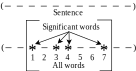
\includegraphics{RATstat/luhn-score.pdf} % % %[width=140mm]
 \caption[Score d'une phrase selon Luhn]{Score d'une phrase selon Luhn \cite{58-luhn}.}
 \label{fig:luhn-score}
\end{center}
\end{figure}

\section{Pré-traitement}
\label{sec:pre-trait}

%Resource Lean and Portable Automatic Text Summarization page 24 \\
Le pré-traitement dans le résumé automatique de textes (ou la recherche d'information en général) est une tâche très importante, liée à la langue traitée. 
En discutant le travail de Luhn, nous avons introduit les différentes étapes utilisées dans le pré-traitement. 
%Nous avons vu son importance en discutant le travail de Luhn.
Ces étapes étant la normalisation, la segmentation, la radicalisation, la suppression de mots vides, etc., sont des techniques du TALN \cite{04-brants}. 
Elles sont utilisées par les systèmes de résumé automatique afin de rendre le texte d'entrée plus facile à traiter et de le transformer à un standard qui est utilisé comme entrée au module de traitement. 
%Natural Language Processing in Information Retrieval.pdf

\subsection{Normalisation}

 %Church, K.: One Term or Two? In: Proceedings of SIGIR 1995, pp. 310–318 (1995)
La normalisation est la procédure qui transforme un document dans un format standard plus facile à manipuler. 
Par exemple, un document peut contenir les mots équivalents "Mr.", "Mr", "mister", et "Mister", qui peuvent tous être normalisés en un seul mot. 

%Un des algorithmes pour la normalisation de la langue Arabe est celui de [Larkey et al., 2002], procédé comme suite: 
Parmi les opérations effectuées dans cette étape:
\begin{itemize}
\item Suppression des caractères spéciaux et des chiffres. 
\item Remplacement de certains mots équivalents, comme les abréviations (voir l'exemple précédent). 
\item Dans certaines langues comme la langue Arabe, élimination des diacritiques. 
\item Remplacement de certains caractères, comme l'algorithme de \cite{02-larkey-al} destiné à diminuer les variations qui peuvent exister lors de l'écriture d'un mot en arabe. 
\item La suppression de certaines formes de style, comme celles des pages Web. 
\end{itemize}
La radicalisation est aussi une forme de normalisation, elle sera discutée ultérieurement (voir la section \ref{sec:stemming}).

\subsection{Segmentation}

Dans le résumé par extraction, il est nécessaire de décider sur quelle granularité nos segments vont être extraits, c.-à-d.  la taille de chaque unité extraite pour former le résumé. 
Elle peut être un paragraphe, une phrase, ou une clause; bien que dans la plupart des cas, l'extraction se fait au niveau de phrase. 
Dans l'approche statistique, les traitements sont exécutés sur les mots qui doivent être segmentés eux aussi, on appelle ça en anglais: Tokenization. 

\subsubsection{Segmentation du texte en phrases}

%La détection des limites en utilisant la ponctuation et le contexte
Dans la plupart des langues écrites, les phrases sont délimitées par des marques de ponctuation comme le point, le point d'exclamation, le point d'interrogation. 
La phrase est définie par une clause qui commence par une lettre majuscule et se termine par un des trois marques de ponctuation précédentes \cite{90-nunberg}. 
Mais, il existe des cas où cette définition ne peut pas être appliquée: 
\begin{itemize}
\item Le point peut être utilisé dans les abréviations, par exemple "Mr.", "Dr.", "etc.", etc., qui se trouvent dans la plupart des cas au milieu d'une phrase. 
\item Les phrases peuvent être délimitées par plusieurs autres marques de ponctuation \cite{10-palmer}. 
Il existe des cas où des phrases sont délimitées par des marques autres que les points, comme par exemple les virgules utilisées par les séquences d'actions. 
\item Dans des langues, comme le Thaï, il n'existe pas de ponctuation pour différencier les limites de phrases. 
\end{itemize}

Plusieurs facteurs contextuels ont été proposés pour aider à la segmentation en phrases, comme \cite{10-palmer}:
\begin{itemize}
\item Distinction de la casse: les mots commençant par une lettre majuscule donnent une information sur les limites de phrases. 
Les phrases commencent toujours par une lettre en majuscule.

\item Parties du discours (Part of speech): \cite{97-palmer-hearst} ont prouvé que l'utilisation des parties de discours qui entourent une marque de ponctuation avec un algorithme d'apprentissage, peuvent aider à détecter les limites de phrases. 

\item Longueur du mot: La longueur de mots avant et après un point, est utilisée par \cite{89-riley}, comme un critère contextuel. 

\item Les suffixes: \cite{80-muller-al} utilisent l'analyse morphologique pour identifier les suffixes, et de ce fait filtrer les mots qui ne sont pas des abréviations. 
Ceci est utilisé pour identifier les mots qui ne figurent pas dans la liste des abréviations. 

\item Préfixes et suffixes: \cite{97-reynar-ratnaparkhi} utilisent les préfixes et les suffixes des mots entourant la marque de ponctuation, comme un critère contextuel. 
\item Les classes des abréviations: \cite{89-riley} et \cite{97-reynar-ratnaparkhi} divisent les abréviations sur des catégories comme les titres (qui ne peuvent pas être à la fin de phrase, comme \textit{Mr.}, \textit{Dr.}, etc.) et les indicatifs corporatifs (qui peuvent être à la fin de phrase, comme \textit{Corp.}, \textit{S.p.A.}, etc.). 

\item Les noms propres: \cite{02-mikheev} utilise la présence des noms propres à droite du point comme critère. 
\end{itemize}

%Les différents algorithmes de détection de limites
Pour détecter les limites de phrases, il existe deux approches: l'approche basée sur les règles manuelles, et l'approche par apprentissage. 
La première approche est la plus ancienne et la plus utilisée \cite{10-palmer} parmi ces deux approches, pour déterminer les limites de phrases. 
Elle utilise une grammaire régulière définie manuellement, avec une liste des abréviations et des noms propres. 
Un des algorithmes basés sur les expressions régulières, est le système d'extraction de l'information \textit{Alembic} développé par \cite{95-aberdeen-al}. 
Il contient des différents modules qui tentent de classifier toute sorte de marque de ponctuation en identifiant le point dans les nombres, les expressions de date et de temps, et les abréviations. 
Il utilise une liste de 75 abréviations et une série de plus de 100 règles manuelles. 
Cette approche est développée pour un corpus et une langue spécifique et se base sur les listes de mots spécifiques pour une langue.
Ainsi, pour l'appliquer sur une autre langue il faut les redéfinir à nouveau. 

La première approche requiert un grand effort pour écrire les règles de détection les délimiteurs et la préparation de la liste des abréviations. 
Les méthodes par apprentissage tentent de définir ces règles de manière automatique, ceci permettra de varier les langues, les applications, et les genres. 
Le premier travail utilisant cette approche pour la segmentation en phrases, est celui de \cite{89-riley}. 
Sa méthode utilise les arbres de régression \cite{84-breiman-al} pour classifier les points selon des critères contextuels concernant les mots qui précèdent et qui suivent les points. 
Ces critères contextuels comportent: la longueur du mot, la ponctuation après le point, les classes d'abréviation, la casse du mot, et la probabilité que le mot ayant place au début ou à la fin de la phrase. 
Les algorithmes basant sur l'approche par apprentissage, sont nécessaires pour fournir des traitements robustes sur une variété de textes et de langues. 

\subsubsection{Segmentation du texte en mots (Tokenization)}

La segmentation de mots est une étape nécessaire pour exécuter les traitements statistiques. 
Dans la plupart de systèmes d'écriture, les mots sont séparés par des espaces. 
Un simple algorithme de segmentation de mots considère tous les caractères consécutifs précédés et suivis par un espace, comme un mot. 
Cette convention est sujet de plusieurs problèmes:
%
\begin{itemize}
%
\item Les marques de ponctuation sont considérées comme un terme séparé. 
Mais dans le cas du point, on peut trouver qu'il peut être attaché à un autre terme, comme les abréviations qui se terminent toujours par un point. 
%
\item Les marques de citation (\textquotedblleft \textquotedblright \textquoteleft \textquoteright) sont utilisées pour spécifier le début et la fin d'une citation. 
Les guillemets de citation et l'apostrophe ont le même caractère, et donc on ne peut pas déterminer immédiatement si la marque est un guillemet ou une apostrophe. 
%
\item L'apostrophe est une source d'ambiguïté dans la segmentation de mots. 
Dans l'anglais, l'apostrophe peut être utilisée avec un "\textit{s}" dans la forme possessive (\textit{Karim's thesis}), dans la contraction du verbe "\textit{is}" (\textit{she's}, \textit{it's}, etc.), comme elle peut être utilisée dans le pluriel de certains mots (\textit{I.D.'s}, \textit{1980's}, etc.). 
L'apostrophe est aussi utilisée dans les cas de contraction. 
Dans l'anglais, les contractions "\textit{I'm}" et "\textit{we've}" sont segmentés comme "\textit{I am}" et "\textit{we have}" respectivement. 
Pour le français, on peut citer un ensemble de contractions, y compris: la contraction des articles (\textit{l'homme}, \textit{c'était}), la contraction des pronoms (\textit{j'ai}, \textit{je l'ai}), et autres formes (\textit{n'y}, \textit{qu'ils}, \textit{d'ailleurs}).
%
\item Certaines langues contiennent des mots composés, soit en attachant un mot à l'autre, soit par trait d'union. 
Dans l'allemand, il est commun d'utiliser la composition des mots: nom-nom (\textit{Lebensversicherung}, assurance vie), adverbe-nom (\textit{Nichtraucher}, non-fumeur), et préposition-nom (\textit{Nachkriegszeit}, période d'après-guerre). 
Autres langues utilisent le trait d'union, comme l'anglais (\textit{end-of-file}, \textit{classification-based}, etc.), et le français (\textit{va-t-il}, \textit{c'est-à-dire}, \textit{celui-ci}, etc.). 
%
\end{itemize}

Il existe des langues non-segmentées (tous les mots sont attachés), comme le chinois, le japonais, et le thaï.
Les techniques pour segmenter les mots pour ces langues sont différentes à celles utilisées pour les langues avec espace. 
Il existe trois approches pour la segmentation: Statistique, lexicale basée sur des règles, et une autre approche hybride entre ces deux. 

L'approche statistique utilise des données comme l'information mutuelle entre les caractères, compilée d'un corpus d'apprentissage, pour déterminer quels sont les caractères les plus probables pour former un mot. 
L'approche lexicale utilise des règles encodées manuellement sur la langue, comme l'information syntaxique et sémantique, les structures communes de phrases, et les règles morphologiques, pour définir la segmentation. 
Le système d'écriture chinois est constitué de milliers de caractères appelés \textit{Hanzi}, avec des mots d'un ou plusieurs caractères \cite{10-palmer}. 
Il existe une multitude d'algorithmes pour la segmentation de textes chinois  \cite{96-sproat-al,97-palmer,98-hockenmaier-brew,00-teahan-al,05-gao-al}.
Par contre, la langue japonaise contient plusieurs systèmes d'écriture (voir la figure \ref{fig:jap-writing}), qui rend la segmentation plus facile comme les transitions entre les groupes de caractères donnent des informations sur les limites de mots. 
Parmi les travaux de segmentation pour le japonais, on peut citer les deux systèmes célèbres \textit{JUMAN} \cite{94-matsumoto-nagao} et \textit{Chasen} \cite{07-matsumoto-al}. 
%
\begin{figure}[ht]
\begin{center}
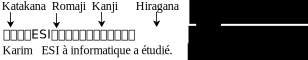
\includegraphics{RATstat/jap-writing.pdf} % % %[width=140mm]
 \caption{Les systèmes d'écriture Japonais.}
 \label{fig:jap-writing}
\end{center}
\end{figure}
%
Pour le Thaï, il comporte moins de caractères avec des mots plus longs que ceux de chinois et de japonais. 
Une bonne segmentation dans cette langue demande une bonne connaissance sur sa lexique et morphologie \cite{96-asanee-al,97-meknavin-al,02-aroonmanakun}.

\subsection{Radicalisation} %Racine du mot
\label{sec:stemming}

Dans tout texte, le même mot pouvait se produire dans des différentes variantes morphologiques. 
Dans la plupart des cas, ces formes lexicales possèdent des interprétations sémantiques similaires, et peuvent être considérées comme équivalentes pour les systèmes de gestion d'information.
Afin que ces systèmes puisent utiliser ces formes comme un seul concept, on utilise souvent un algorithme pour trouver la racine du mot, appelé radicalisateur (\textit{Stemmer}).

La radicalisation tente de réduire un mot vers son radical. 
L'effet n'est pas seulement celui de réduire les différentes variantes d'un terme vers une seule forme représentative, mais aussi de réduire la taille du vocabulaire utilisée par le système pour stocker les représentations. 
Dans la plupart des cas, la petite taille du dictionnaire nous permet de préserver l'espace du stockage et le temps de traitement, ainsi de rendre le document moins bruyant, plus compact, et plus souple \cite{07-hassel}. 

Le résultat d'une radicalisation peut être un mot qui n'a aucun sens, mais qui est commun entre les mots ayant le même sens. 
Le rendement d'une radicalisation dépend sur la racine résultat; il est bon si les différents mots avec le même sens de base ont la même racine, et si les mots qui n'ont pas le même sens sont séparés. 
Selon ces conditions, on peut avoir deux types de problèmes \cite{07-hassel}:
\begin{itemize}
\item Sur-radicalisation: se passe lorsque deux mots sont donnés la même racine, mais en réalité ils ne l'ont pas. 
\item Sous-radicalisation: se passe lorsque les mots qui doivent avoir la même forme de base, ne l'ont pas. 
Par exemple, les deux mots "running" et "ran" doivent avoir la même racine "run", mais le système nous donne "run" et "ran" en ordre.
\end{itemize}

Dans la radicalisation, il existe deux grandes approches \cite{04-brants}: radicalisation linguistique/avec-dictionnaire et radicalisation de style Porter \cite{97-porter}. 
La première méthode donne un meilleur résultat, mais exige un coût d'implémentation et de traitement très élevé pour une petite couverture. 
La deuxième méthode est meilleure de point de vue implémentation et coût de traitement pour une performance acceptable.
Des radicalisateurs ont été développés pour plusieurs langues, ayant compris Malais \cite{00-tai-al}, Latin \cite{96-greengrass-al}, Indonésien \cite{01-sn-bressan}, Suédois \cite{01-carlberger-al}, Néerlandais \cite{96-kraaij-pohlmann}, Allemand \cite{01-monz-rijke}, Français \cite{01-moulinier-al}, Slovène \cite{92-popovic-willett}, Turc \cite{96-ekmekcioglu-al}, et Arabe \cite{02-larkey-al}.

\subsection{Suppression des mots vides}

La suppression de mots vides est une technique commune pour répondre au fait que plusieurs mots dans le document ne contribuent pas particulièrement dans la description de son contenu, et ne font qu'ajouter de bruit. 
La plupart des systèmes de recherche d'information et de résumé automatique, suppriment les mots vides avant de traiter les documents. 
Ceci va augmenter la performance du système, mais éventuellement peut causer des problèmes pour traiter certains cas comme les suivants (les mots vides sont en gras):
\begin{itemize}
\item \textbf{To be or not to be}
\item \textbf{Will and} Grace
\end{itemize}
Pour la première phrase, en supprimant les mots vides, on n'aura aucun mot à traiter, puisque tous les mots sont des mots vides, et donc cette phrase ne participera jamais dans le traitement. 
La deuxième phrase contient le mot "\textit{Will}" qui est un nom, mais le système le considère comme le verbe "\textit{will}" présent dans la liste des mots vides pour l'anglais. 

\section{Critères statistiques}
\label{sec:crit-stat}

Une fois qu'on procède au pré-traitement du texte source, on aura les informations nécessaires pour effectuer le traitement (dans ce cas l'extraction des unités saillantes). 
Pour repérer les unités saillantes (expressions, propositions, phrases, paragraphes) dans le texte, il existe un ensemble de critères statistiques identifiés dans les travaux précédents portant sur le résumé automatique statistique. 

\subsection{Fréquence des mots}

La fréquence des mots (\textit{tf: term frequency}) est le critère le plus utilisé; il a été utilisé par Luhn \cite{58-luhn} pour calculer le score de chaque phrase. 
Il correspond au nombre de fois que la racine d'un mot $ m $ apparaît dans un document $ d $. 
Pour calculer la fréquence d'un mot $ m $, on calcule le nombre d'apparition de toutes ces formes dans le document en question, comme par exemple: "\textit{différencier}", "\textit{différent}", "\textit{différenciation}", etc.
Souvent, le nombre de mots est divisé par le nombre total de mots dans le document, ceci afin de ne pas favoriser les documents longs; ceci peut être représenté par l'équation \ref{eq:tf}.
%
\begin{equation}
\label{eq:tf}
tf(m, d) = \frac{|m|_d}{\sum_{i = 1}^{|d|}{|m_i|_d}}
\end{equation}
Où: 
$ tf(m, d) $ est la fréquence du mot $ m $ dans le document $ d $. 
$ |m|_d $ est le nombre d'occurrences de $ m $ dans le document $ d $. 
$ |d| $ est le nombre de mots différents dans le document $ d $. 

En utilisant la fréquence de mots, on peut rapidement détecter qu'il y a un problème pour les documents du même domaine. 
Dans un domaine donnée, l'informatique par exemple, certains mots sont fréquemment utilisés (exp. ordinateur, informatique, etc.) et donc ces mots vont avoir des grandes fréquences malgré qu'ils ne représentent pas le thème du document. 
Pour contourner ce problème, Salton \cite{73-salton-yang} définit un autre critère appelé $ tf*idf $. 
Le critère $ tf*idf $ exprime qu'un mot est plus important lorsqu'il est plus fréquent dans le document analysé et peu fréquent dans le corpus de documents analysés. 
La propriété $ idf $ s'appelle "\textit{la fréquence inverse de documents}" (en Anglais: \textit{inverse documents frequency}). 
La logique derrière cette propriété est que le mot est plus important lorsqu'il est moins probable de se trouver dans les documents du corpus traité (concernant certain domaine) d'où le mot \textit{inverse} (voir l'équation \ref{eq:idf}).
%
\begin{equation}
\label{eq:idf}
idf(m) = log{\frac{|D|}{|\{d: m \in d\}|+1}}
\end{equation}
Où: 
\begin{itemize}
\item $ |D| $ est le nombre des documents dans le corpus;
\item $ |\{d: m \in d\}| $ est le nombre des documents contenants le mot $ m $.
\end{itemize}
Donc, le facteur $ tf*idf $ va être écrit comme dans l'équation \ref{eq:tf-idf}.
\begin{equation}
\label{eq:tf-idf}
tf*idf(m, d) = tf(m, d)*idf(m)
\end{equation}

\subsection{Position dans le texte}

La position des mots et des phrases dans le texte peut être un bon indicateur de leurs importances. 
Celle-ci peut faire référence à la position de mots dans la phrase \cite{58-luhn}, où bien à la position de la phrase par rapport à une unité (document, section, paragraphe, etc.)\cite{58-baxendale,69-edmundson,97-lin-hovy,04-nobata-sekine}.
%Par exemple, dans les articles scientifiques, l'introduction et la conclusion contiennent des phrases qui résument tous le document. 
Par exemple, dans un paragraphe, les premières et les dernières phrases sont les plus importantes.
Ceci a été prouvé par Baxendale \cite{58-baxendale}, lorsqu'il a utilisé un corpus de 200 paragraphes pour tester l'impact de la position de phrases dans un paragraphe sur son importance. 
Il a trouvé que dans 85\% la première phrase est la plus importante pour le paragraphe, et 7\% pour la dernière. 
Edmundson \cite{69-edmundson}, ensuite, a explicité la position en se basant sur l'hypothèse: "les phrases du thème tendent à apparaître très tôt ou très tard dans un document ou dans ses paragraphes" ("\textit{topic sentences tend to occur very early or very late in a document and its paragraphs}").
Les auteurs de \cite{97-lin-hovy} vont dans le même sens, ils définissent des algorithmes pour l'identification automatique de la position des phrases les plus importantes, mais cette fois en fonction du thème traité.

Dans \cite{04-nobata-sekine}, les auteurs définissent rois méthodes pour le calcul du score de la phrase en utilisant sa position (voir les équations \ref{eq:nobota-pos-1}, \ref{eq:nobota-pos-2}, et \ref{eq:nobota-pos-3}).
%Supposant qu'il y a $ n $ phrases dans le texte d'entrée, pour chaque équation le score de phrase $ p_i $, dont $ i $ est sa position dans le texte, est $ Score_{pos}(p_i) $. 
La première méthode donne $ 1 $ pour les $ N $ premières phrases, et $ 0 $ pour les autres. 
%Sachant que $ N $ est le nombre de phrases dans le résumé.
\begin{equation}
\label{eq:nobota-pos-1}
Score_{pos}(p_i) = \left\lbrace 
\begin{array}{lll}
1 & si & (i<N) \\
0 & sinon & \\
\end{array}
\right. 
\end{equation}
La deuxième méthode suppose que les phrases ont une importance inversement proportionnée à leurs positions. 
\begin{equation}
\label{eq:nobota-pos-2}
Score_{pos}(p_i) = \frac{1}{i}
\end{equation}
La troisième méthode suppose que les phrases dans le début et dans la fin du document sont les plus importantes.
\begin{equation}
\label{eq:nobota-pos-3}
Score_{pos}(p_i) = \max(\frac{1}{i}, \frac{1}{n-i+1})
\end{equation}
Selon les auteurs, la deuxième méthode donne un résultat meilleur que ceux des autres méthodes.

Dans \cite{09-abdelfattah-ren}, les auteurs utilisent la position des phrases dans le paragraphe (et pas dans la totalité de texte). 
Ils supposent que les premières phrases du paragraphe sont les plus importantes, en prenant cinq phrases comme la position maximale (voir l'équation \ref{eq:abdelfattah-pos}). 
\begin{equation}
\label{eq:abdelfattah-pos}
Score_{pos}(p_i) = \left\lbrace 
\begin{array}{lll}
6 - i & si & (i \leq 5)\\
0 & sinon &  \\
\end{array}
\right. 
\end{equation}
Où: $ i $ est la position de phrase dans le paragraphe.

\subsection{Mots du titre et des sous-titres}

Dans \cite{69-edmundson}, l'auteur se base sur l'hypothèse que le titre véhicule le thème du document.
En plus, lorsque l'auteur divise le document en sections, il les résume en leurs choisissant les entêtes (titres de sections) appropriées. 
En suivant cette hypothèse, les phrases importantes sont celles contenant des mots du titre ou des sous-titres.
Bien évidemment, les mots du titre ont plus de poids que ceux des sous-titres.
Dans le travail de \cite{88-salton-buckley}, les auteurs propose d'utiliser le titre comme une requête pour toutes les phrases du document; ensuite la similarité cosinus est calculée entre chaque phrase et le titre. 

%[Ishikawa et al., 2001]
En se basant sur la fréquence de mot, \cite{01-ishikawa-al} proposent une méthode qui prend en considération les mots appartenant au titre. 
En effet, lorsqu'un mot appartient au titre, sa fréquence va être multipliée par un nombre $ A > 1 $. 
Ainsi, le score d'une phrase $ p_i $: $ Score_{titre}(p_i) $ est donné par l'équation \ref{eq:ishikawa-head}.
\begin{equation}
\label{eq:ishikawa-head}
Score_{titre}(p_i) = \sum_{\{m\} \in p_i}{\alpha(m) * tf(m)}
\end{equation}
Où: 
\begin{equation}
\label{eq:ishikawa-head2}
\alpha(w) = \left\lbrace 
\begin{array}{lll}
A > 1 & si & w \in Titre \\
1 & sinon & \\
\end{array} 
\right. 
\end{equation}

%04-nobata-sekine
Dans \cite{04-nobata-sekine}, deux méthodes sont utilisées pour calculer le score des phrases en se basant sur les mots du titre. 
Pour chaque phrase $ p_i $ et sachant le titre $ T $,  le score de cette phrase est donné par $ Score_{titre}(p_i) $. 
La première méthode utilise le $ tf*idf $ des mots de titre, comme il est indiqué dans l'équation \ref{eq:nobta-head-1}.
\begin{equation}
\label{eq:nobta-head-1}
Score_{titre}(p_i) = \frac{\sum_{m \in T \bigcap p_i}{\frac{tf(m)}{tf(m)+1} idf(m)}}
{\sum_{m \in T}{\frac{tf(m)}{tf(m)+1} idf(m)}}
\end{equation}
La deuxième méthode utilise les entités nommées et la fréquence de mots $ tf $. 
Pour une entité nommé $ e $, l'équation \ref{eq:nobta-head-2} est utilisée pour calculer le score d'une phrase $ p_i $ en se basant sur le titre.
\begin{equation}
\label{eq:nobta-head-2}
Score_{titre}(p_i) = \frac{\sum_{e \in T \bigcap p_i}{\frac{tf(e)}{tf(e)+1}}}
{\sum_{e \in T}{\frac{tf(e)}{tf(e)+1}}}
\end{equation}
Selon les auteurs, la deuxième méthode donne un meilleur résultat. 

\subsection{Longueur de phrase}

Ce critère est utilisé pour pénaliser les phrases qui sont trop petites, vu que ces phrases ne serons pas incluses dans le résumé \cite{95-kupiec-al}. 
Le score pour ce critère est la longueur normalisée de phrase; qui est la proportion entre le nombre de mots dans la phrase et le nombre de mots dans la phrase la plus longue dans le document \cite{02-neto-al,04-nobata-sekine}.

Dans le travail de \cite{04-nobata-sekine}, deux méthodes sont utilisées. 
La première donne un score égale au longueur de phrase divisée par une longueur $ L_{max} $ prédéfinie, si la longueur de phrase est supérieure à $ L_{max} $ on lui attribue un score égale à $ 1 $ (voir l'équation \ref{eq:nobota-len-1}). 
\begin{equation}
\label{eq:nobota-len-1}
Score_{long}(p_i) = \left\lbrace 
\begin{array}{lll}
\frac{L_i}{L_{max}} & si & (L_i \leq L_{max}) \\
1 & sinon & \\
\end{array}
\right. 
\end{equation}
La deuxième méthode donne un score négatif afin de pénaliser les phrases qui sont plus courtes que $ L_{min} $ (voir l'équation \ref{eq:nobota-len-2}). 
\begin{equation}
\label{eq:nobota-len-2}
Score_{long}(p_i) = \left\lbrace 
\begin{array}{lll}
0 & si & (L_i \geq L_{min}) \\
\frac{L_i - L_{min}}{L_{min}} & sinon & \\
\end{array}
\right. 
\end{equation}
Selon les auteurs, la deuxième méthode donne un meilleur résultat. 

Une autre formule pour calculer le score d'une phrase $ p_i $ dans un document $ d $ en utilisant sa longueur, est utilisée dans \cite{09-abdelfattah-ren} (voir l'équation \ref{eq:abdelfattah-len}). 
\begin{equation}
\label{eq:abdelfattah-len}
Score_{pos}(p_i) = \frac{|p_i| * |\{P: P \in d\}|}{|d|}
\end{equation}
Où: 
$ |p_i| $ et $ |d| $ sont les nombres de mots dans la phrase $ p_i $ et le document $ d $ respectivement. 
$ |\{P: P \in d\}| $ est le nombre de phrases dans le document $ d $. 

\subsection{Mots indicatifs} % indicatifs clés
%the presence of cue words and expressions such as “important”, “definitely”,  “in particular” (all positive), and “unclear”, “perhaps”, “for example” (all negative) [Edmundson 1969; Rush et al. 1971]; (93-paice-jones)

Les méthodes utilisant les mots indicatifs (\textit{cue words}), sont basées sur l'hypothèse que la pertinence d'une phrase est affectée par la présence de mots comme "\textit{significatif}", "\textit{impossible}", et "\textit{difficilement}" \cite{69-edmundson}. 
Ces méthodes utilisent des mots sauvegardés dans un dictionnaire extrait à partir d'un corpus. 
Le dictionnaire de mots clés contient trois sous-dictionnaires: Les mots \textit{Bonus}, qui sont pertinents positivement (\textit{important}, \textit{précisément}, \textit{particulièrement}, etc.); Les mots \textit{Stigmates}, qui sont plutôt pénalisant (\textit{obscurément}, \textit{peut-être}, etc.); et les mots \textit{Null}, qui ne sont pas indicatifs. 
Le score total pour une phrase $ p_i $ basé sur ce critère, est la somme des poids $ cue(m) $ pour ses mots constituants $ m $. 
Ceci est indiqué dans l'équation \ref{eq:edmundson-cue}, où $ cue(m) $ est le poids du mot $ m $ par rapport au dictionnaire de mots clés. 
\begin{equation}
\label{eq:edmundson-cue}
Score_{cue}(p_i) = \sum_{m \in p_i}{cue(m)}
\end{equation}
Sachant que:
\begin{equation}
\label{eq:edmundson-cue2}
cue(m) = \left\lbrace 
\begin{array}{lll}
b > 0 & si & (w \in Bonus) \\
\delta < 0 & si & (w \in Stigma) \\
0 & sinon & 
\end{array} 
\right. 
\end{equation}

Dans \cite{09-abdelfattah-ren}, les mots clés positifs sont définis par "les mots fréquemment inclus dans le résumé". 
Le score d'une phrase $ p_i $ en utilisant les mots clés positifs, est donné par l'équation \ref{eq:abdelfattah-cue+}. 
\begin{equation}
\label{eq:abdelfattah-cue+}
Score_{cue}(p_i) = \frac{1}{|p_i|} \sum_{m \in p_i}{tf(m) * P(p_i \in R | m)}
\end{equation}
Où: 
$ P(p_i \in R | m) $ est la probabilité que la phrase $ p_i $ appartienne au résumé $ R $ sachant qu'elle contient le mot $ m $. 
Cette probabilité peut être calculée en utilisant un corpus d'apprentissage (contenant des résumés modèles), et en appliquant l'équation \ref{eq:abdelfattah-prob}. 
\begin{equation}
\label{eq:abdelfattah-prob}
P(p_i \in R | m) = \frac{P(m | p_i \in R) * P(p_i \in R)}{P(m)}
\end{equation}
Par conséquent, les mots clés négatifs sont les mots peu probables d'être dans un résumé (voir l'équation \ref{eq:abdelfattah-cue-})
\begin{equation}
\label{eq:abdelfattah-cue-}
Score_{cue}(p_i) = \frac{1}{|p_i|} \sum_{m \in p_i}{tf(m) * P(p_i \notin R | m)}
\end{equation}

\subsection{Expressions saillantes}
%These are commonly occurring structures which explicitly state that the sentences containing them have something important to say about the subject matter or the 'message' of the document. 

Les expressions saillantes sont des structures, lorsqu'elles se produisent dans une phrase, expriment explicitement que cette phrase contient une information importante à propos du sujet ou un "message" du document \cite{81-paice}. 
Par exemple "\textit{Le but principal de cet article est de vérifier ...}", "\textit{Dans cet article, une méthode est décrite pour ...}", etc.
D'après Paice, l'identification des expressions saillantes n'est pas une tâche simple (une comparaison de chaînes de caractères ne suffit pas), à cause des raisons suivantes:
\begin{itemize}
\item On ne peut pas lister toutes les expressions saillantes à cause des variations qui peuvent exister. 
Par exemple, les expressions suivantes ont la même structure: "\textit{This article is concerned with ...}", "\textit{Our paper deals with ...}", "\textit{The present report concerns ...}" et "\textit{The following discussion is about ...}". 
Donc, la solution est d'utiliser des modèles contenant des mots appelés \textit{les paradigmes} (prototypes, modèles). 

\item En utilisant les modèles, il parait qu'il existe des mots qui ne figurent pas dans ces modèles malgré qu'ils fassent partie d'une expression indicative. 
La solution est d'utiliser des sauts limités entre les paradigmes d'un modèle donné.

\item Il existe des mots qui sont optionnels, mais qui ajoute un poids lorsqu'on les utilise, comme le mot "\textit{here}" dans l'expression "\textit{The purpose \textbf{here} is to ...}". 
On peut définir de multiples chemins dans le modèle. 

\item Enfin, les mots peuvent avoir plusieurs variations, ce problème peut être résolu en utilisant leurs racines dans les modèles. 
\end{itemize}
La figure \ref{fig:paice-template} représente un modèle pour détecter les expressions saillantes, où les mots sont les paradigmes. 
Les limites de sauts entre les paradigmes sont présentées comme [3]. 
Le gain de poids de l'expression est présenté comme +2. 
Les paradigmes suivis par (?) sont optionnels.
%
\begin{figure}[ht]
\begin{center}
\includegraphics{RATstat/paice-template.pdf} % % %[width=140mm]
 \caption[Un des modèles pour détecter les expressions saillantes] %
 {Un des modèles pour détecter les expressions saillantes (version simplifiée) \cite{81-paice}.}
 \label{fig:paice-template}
\end{center}
\end{figure}

\subsection{Combinaison des critères}

Tous ou une partie des critères précédemment présentés sont combinés sous forme d'une combinaison linéaire en les attribuant un poids à chaque critère (voir l'équation \ref{eq:combin-crit}).
\begin{equation}
\label{eq:combin-crit}
Score(p_i) = \sum_{c \in Criteres}{\alpha_c * Score_c(p_i)}
\end{equation}
Pour un poids $ \alpha_c $ d'un critère $ c $, la définition de la valeur était manuelle ou intuitive, dans les premiers travaux de résumé automatique. 
Dans \cite{69-edmundson}, l'auteur utilise quatre critères: les mots indicatifs (\textit{C: Cue}), la fréquence de mots (\textit{K: Key}), les mots de titre (\textit{T: Title}), et la position (\textit{L: Location}). 
Les quatre critères précédents sont combinés pour calculer le score de la phrase ($ S = \alpha_lC + \alpha_2K + \alpha_3T + \alpha_4L $), ce qui nous donne 15 combinaisons différentes. 
La figure~\ref{fig:edmundson-score} représente le pourcentage moyen de pertinence des combinaisons les plus intéressantes, ainsi que l'intervalle entre le pourcentage moyen moins et plus l'écart standard.
%with the intervals encompassing the sample mean plus and minus one sample standard deviation. 
%
\begin{figure}[ht]
\begin{center}
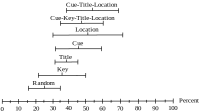
\includegraphics{RATstat/edmundson-score.pdf} % % %[width=140mm]
 \caption[Les moyennes des scores de pertinence pour chaque combinaison de critères]{Les moyennes des scores de pertinence pour chaque combinaison de critères \cite{69-edmundson}.}
 \label{fig:edmundson-score}
\end{center}
\end{figure}
Avec l'avènement des techniques d'apprentissages, ces derniers ont été utilisés dans le but d'estimer les poids de critères (voir la section~\ref{sec:appentissage}). 
%Plusieurs techniques d'apprentissage ont été utilisés: les algorithme génétiques, la régression mathématique, réseau de neurone \cite{09-abdelfattah-ren}.

\section{Amélioration de l'approche statistique}

Le choix de différents poids pour chaque critère est difficile, puisque chaque genre de document se base sur des critères spécifiques plus que d'autres. 
Par exemple, dans un document de presse, le critère de position est très important puisque l'information pertinente se trouve au début, donc il faut donner un poids élevé à ce critère pour ce genre de documents. 
Une autre limite est le manque de ressources linguistiques en plus du bruit introduit par la considération de la totalité des phrases pour ne garder que l'information pertinente.
C'est pourquoi plusieurs recherches ont été menées afin d'améliorer l'approche statistique.

\subsection{Techniques linguistiques}

Il existent des travaux qui intègrent des données linguistiques avec l'approche statistique, notamment en utilisant les graphes de similarité \cite{02-neto-al,09-abdelfattah-ren}, ou en utilisant les parties du discours (\textit{part of speech})\cite{96-kraaij-pohlmann,02-neto-al}, etc.
Après l'application de ces techniques, on obtient des propriétés linguistiques qui peuvent être traitées statistiquement en comptant leurs fréquences, par exemple le nombre de noms dans une phrase.

La cohésion entre les phrases est une propriété importante.
En effet, plus un résumé contient des phrases liées, plus sa qualité augmente. 
Dans cette logique, \cite{09-abdelfattah-ren} utilise le nombre des arcs dans le graphe de similarité de toutes les phrases, pour calculer l'importance d'une phrase. 
L'équation \ref{eq:abdelfattah-arcs} représente le score de ce critère, où $ G =  \{S, A\} $ est le graphe de similarité entre les phrases, $ S $ est l'ensemble de sommets (phrases), et $ A $ est l'ensemble des arcs.
\begin{equation}
\label{eq:abdelfattah-arcs}
Score_{\#arcs}(p_i) = |\{ p_j : a(p_i, p_j) \in A / p_j \in S, p_i \neq p_j \}|
\end{equation}

Dans \cite{02-neto-al}, les auteurs utilisent la somme des poids (de similarité) des arcs reliant la phrase avec le reste des phrases. 
Supposant que $ W(x, y) $ est le poids de l'arc liant $ x $ à $ y $, i.e. la similarité entre les phrases $ x $ et $ y $, le score de ce critère est donné par l'équation \ref{eq:arcs-weight}.
\begin{equation}
\label{eq:arcs-weight}
Score_{poids-arcs}(p_i) = \sum_{p_j \in S} W(p_i, p_j) / a(p_i, p_j) \in A , p_i \neq p_j
\end{equation}

Un autre traitement linguistique qui a prouvé son utilité pour le résumé automatique (et la recherche d'information) est l'intégration des parties de discours. 
Dans \cite{96-kraaij-pohlmann}, des expériences sont faites pour vérifier l'effet des différentes parties de discours sur la recherche d'information, en les utilisant comme des termes de requête. 
Pour le Néerlandais, ils trouvent que 58\% des termes réussis sont des noms, 29\% sont des verbes, 13\% sont des adjectifs. 
Dans le résumé automatique, l'occurrence des noms propres est utilisée par \cite{02-neto-al} comme critère. 
Ceci est motivé par le fait que les noms propres, qui font référence à des gens ou des places, sont des indices que la phrase est pertinente pour le résumé.
Dans ce travail, on considère seulement la présence ou non de noms propres et pas leurs nombres. 

\subsection{Apprentissage}
\label{sec:appentissage}

L'objectif principal de tout algorithme d'apprentissage automatique est d'apprendre, d'identifier un ensemble de règles depuis un corpus de documents, ces règles sont ensuite appliquées sur le ou les textes en entrée du système de résumé. 
Dans ce type de systèmes, on définit deux principales phases  qui sont:  la phase d'entraînement et la phase de tests. 
Dans la première phase, l'ensemble des caractéristiques sont extraites du corpus d'entraînement pour générer, ensuite, des règles de classification en utilisant un algorithme d'apprentissage.
Dans la deuxième phase, ces règles sont appliquées sur le corpus de test afin de générer les résumés correspondants. 
Tous les travaux précédents suivent les mêmes phases, la différence réside dans le choix de l'algorithme d'apprentissage le plus approprié \cite{95-kupiec-al,02-osborne,05-yeh-al}, le traitement des problèmes liés à la phase d'entraînement tels que l'absence ou la taille réduite des corpus étiquetés \cite{01-amini-gallinari}, la combinaison des critères hétérogènes \cite{08-wong-al,10-yatsko-al}, etc. 

Étant donné un corpus qui contient des documents avec leurs résumés extractifs, on peut utiliser un algorithme d'apprentissage pour estimer qu'une phrase appartient au résumé ou non. 
Les auteurs de \cite{95-kupiec-al} proposent un système de résumé par apprentissage basé sur la classification de Bayes, afin de calculer la probabilité qu'une phrase appartient au résumé, pour enfin réorganiser les phrases selon leurs probabilités et extraire les premières. 
Ainsi, pour chaque phrase $ p_i $, on calcule la probabilité qu'elle peut être sélectionnée dans un résumé $ R $ étant donné le vecteur de critères $ \overrightarrow{f} $ (l'équation \ref{eq:bayes-kupiec}).
\begin{equation}
\label{eq:bayes-kupiec}
P(s_i \in R | \overrightarrow{f}) = %
\frac{\prod_{j = 1}^{|\overrightarrow{f}|} P(f_j | s_i \in R) . P(s_i \in R)}
{\prod_{j = 1}^{|\overrightarrow{f}|} P(f_j)}
\end{equation}
Où: 
$ P(s_i \in R) $ est une constante, et les deux probabilités $ P(f_j | s_i \in R) $ et $ P(f_j) $ peuvent être estimées de corpus d'entrainement en calculant les occurrences.

Le problème majeur avec l'utilisation d'un classificateur bayésien est l'indépendance supposée de critères, Osborne a tenté de résoudre ce problème en utilisant un modèle logarithmique linéaire \cite{02-osborne}. 
L'utilisation de classificateur basé sur le principe du maximum d'entropie (Maxent) donne une performance au-dessous du classificateur Na\"ive-Bayes, mais le surpasse lorsqu'on utilise une probabilité à priori avec Maxent. 
Dans sa version, au lieu de réorganiser les phrases en utilisant leurs probabilités, Osborne utilise un algorithme d'apprentissage pour classifier les phrases dans deux classes: la première contient les phrases de résumé, et la deuxième contient les autres phrases. 

\cite{01-amini-gallinari} tentent d'atténuer les problèmes causés par l'absence de corpus étiquetés, en proposant une méthode auto-supervisée. %; qui ne se base pas sur la disponibilité des corpus libellés pour l'apprentissage. 
Le modèle proposé peut être utilisé dans les résumés généraux, ainsi que dans les résumés par requête. 

Contrairement aux travaux précédents, \cite{05-yeh-al} proposent une méthode qui, au lieu de trouver la probabilité ou la classe d'une phrase, attribue des poids aux critères utilisés en utilisant un corpus d'apprentissage. 
Pour ce faire, ils utilisent un algorithme génétique pour attribuer ces poids (la position de phrase, les mots clés, le centre, et la similarité avec le titre). 
Le score final d'une phrase est la somme des scores de chaque critère multiplié par son poids.

De même, \cite{08-wong-al} proposent une approche par apprentissage afin de combiner des critères hétérogènes. 
Ces critères sont classés en quatre catégories: surface, contenu, pertinence, et événement. 
Les critères de surface sont ceux qui se basent sur les aspects extrinsèques d'une phrase: la position de phrase, la longueur de phrase, etc. 
Les critères de contenu mesurent le score d'une phrase sur la base des mots la composant: les fréquences de mots dans le document.
Les critères de pertinence évaluent la relation d'une phrase avec les autres: la similarité par rapport à la première phrase du document. 
Les critères d'événement représentent les phrases par leurs événements: les verbes et les noms qui comportent des actions.

Dans \cite{10-yatsko-al}, les auteurs vont plus loin et proposent d'utiliser 45 paramètres de différents types : statistiques, de positionnement et discursives afin d'identifier celles qui sont les plus pertinentes pour un genre de document donné (scientifique, presse, et artistique).
En utilisant un algorithme de regroupement (K-Means), ils ont regroupé les documents d'un corpus selon les genres précédents. 
Ensuite, le corpus est utilisé pour identifier les paramètres spécifiques pour chaque genre en attribuant à chacun un poids. 

\subsection{Compression de phrases}

Souvent, les résumés automatiques par extraction contiennent des informations superflues, ceci arrive surtout lorsque le résumé contient des phrases très longues. 
La compression des phrases élimine les parties non nécessaires, et produit des résumés plus abrégés et plus précis. 
Dans \cite{99-jing-mckeown}, les auteurs affirment que la compression de phrases est souvent utilisée par les résumeurs professionnels. 
En effet, on a trouvé que 78\% des phrases de résumé ont été reprises du document d'entrée, et plus de la moitié ont fait l'objet de compression.

Il existe deux approches pour la compression de phrases: la première utilise des techniques linguistiques primitives, et la dernière utilise des techniques statistiques. 
La première utilise des règles syntaxiques et du discours pour déterminer la manière de compression d'une phrase. 
Les règles syntaxiques consistent à la définition de la structure syntaxique de la phrase: son arbre syntaxique ainsi que les constituants à enlever; i.e. ceux avec une faible probabilité.
%La connaissance syntaxique contient la structure syntaxique d'une phrase, et les constituants les moins probables d'être dans le résumé. 
Bien que La connaissance du discours contienne l'information des différentes connections des constituants dans le résumé. 
%
\cite{00-jing} propose un système de compression de phrases, qui utilise de multiples sources de connaissance pour décider quelle expression à éliminer de la phrase extraite. 
Ces sources comportent l'information syntaxique, l'information contextuelle, et des statistiques extraites d'un corpus de résumés professionnels. 
%
Dans le travail de \cite{07-Zajic-al}, la compression des phrases se fait avant leur extraction, et la suppression des constituants se fait intuitivement. 
La compression est exécutée itérativement en supprimant un constituant à la fois. 
À chaque itération la sortie constitue l'entrée d'un module d'extraction, ce dernier utilise six critères pour calculer le score de la phrase.

Dans la deuxième approche, l'approche statistique, les règles de suppression des constituants syntaxique sont apprises par programme, et donc aucune règle linguistique ne doit être fournie comme entrée. 
%
Dans \cite{02-knight-marcu}, deux méthodes basées sur l'approche statistique sont développées: en utilisant le modèle de canal bruyant (\textit{the noisy channel model}), et les arbres de décision. 
Dans la première méthode, l'idée est de supposer que la phrase d'entrée du modèle était courte, qui a été modifiée avec d'autres mots additionnels, d'une manière ou d'une autre.
Étant donnée une phrase longue, le programme produit un arbre syntaxique et émet les différentes hypothèses pour réduire cet arbre. 
Ils mesurent la qualité des arbres en utilisant les scores de \textit{probabilistic context free grammar (PCFG) } et les probabilités de phrase suivant le modèle du langage bi-gramme. 
Ils mesurent la vraisemblance de la transformation d'un arbre large vers un arbre réduit en utilisant des statistiques rassemblés d'un corpus contenant des documents avec leurs résumés. 
La deuxième méthode se base sur les arbres de décision qui sont utilisées pour apprendre les différentes règles appliquées pour réduire les phrases.
%
%Galley and McKeown [65] make two
%significant improvements. They move to a lexicalized head-driven
%approach that allows them to take the lexical heads of constituents
%into account before making deletions. This helps them to avoid deleting
%negation words such as “no” and “not”, which would completely change
%the meaning of the sentence, a problem which Knight and Marcu’s
%approach cannot handle. 

D'autres méthodes ont été proposées pour améliorer la compression de phrases, en utilisant non seulement une seule phrase mais en utilisant les autres qui lui ressembles.
Dans le travail de \cite{08-cohn-lapata}, la tâche de compression de phrases est généralisée.  
Au lieu de raccourcir la phrase en éliminant des mots ou des constituants, ils introduisent des opérations additionnelles comme la substitution, la ré-ordonnancement, et l'insertion.
Dans \cite{10-filippova}, une méthode est développée pour résumer un groupe de phrases reliées avec une phrase plus réduite. 
Dans cette méthode, les phrases sont représentées par un seul graphe, et en prenant le plus court chemin, on obtient un résumé réduit.

\section{Post-traitement}

Dans l'approche statistique, la présentation du résumé est un problème.
En effet, les phrases extraites sont des phrases dispersées au long du texte source, et qui n'ont à priori aucune relation directe. 
Le premier problème à résoudre est la manière dont on organise les phrases extraites pour avoir un résumé cohérent. 
Le deuxième étant l'existence des anaphores dans le résumé.

\subsection{Ordonnancement des phrases} %Assemblage des phrases
%/home/karim/Compression/Nenkova_Overview.pdf

Pour assembler les différentes phrases extraites, il faut d'abord définir leur ordre. 
Cette opération a un impact direct sur la qualité de résumé; un résumé avec des phrases désordonnées est difficile à lire et à comprendre. 
Dans le résumé mono-document, la solution était de préserver l'ordre des phrases dans le document d'origine \cite{99-mckeown-al,00-radev-al,02-lin-hovy}. 
Malgré que, en observant les résumés professionnels, on peut trouver que les phrases ne préservent pas leurs ordres initiaux. 
Dans le résumé multi-document, la tâche est encore plus difficile, puisque l'entrée consiste à plusieurs documents avec des thèmes non nécessairement abordés dans tous ces documents. 
En plus, même pour les phrases des thèmes communs, ces thèmes n'ont pas nécessairement le même ordre dans les documents d'entrée. 

Une des solutions proposées pour le résumé multi-documents est l'ordre de majorité (\textit{Majority Ordering}) \cite{02-barzilay-al}. 
Dans cette solution, on regroupe les phrases similaires provenant de différents documents. 
Ensuite, un graphe qui représente l'ordre local dans l'entrée est construit, où chaque sommet représente un thème. 
Deux sommets sont connectés par un arc, si dans un document, une phrase d'un thème est immédiatement suivie par celle du deuxième thème. 
Le poids de l'arc est le nombre des articles où cet ordre est observé. 
Pour inférer l'ordre global de graphe, un algorithme d'approximation est utilisé. 
Des variations de cette méthode ont été étudiées par plusieurs travaux \cite{05-bollegala-al,08-ji-nie}.

\cite{08-boudin-al} définissent un ensemble d'opérations où différentes expressions sont réécrites à leurs formes standards (acronymes, dates et nombres, références temporelles), les outils de jonction entre les phrases sont éliminés (l'expression "\textit{But, it is ...}" devient "\textit{It is ...}"), ainsi que le contenu parenthésé. 

\subsection{Résolution des anaphores}

Dans le résumé par extraction, les phrases extraites pourraient contenir des références anaphoriques non résolues.
Par exemple, supposant qu'on a le texte suivant:
\begin{quote}
"\textit{\textbf{Cosette} était à sa place ordinaire, assise sur la traverse de la table de cuisine près de la cheminée. 
\textbf{Elle} était en haillons, \textbf{elle} avait ses pieds nus dans des sabots, et elle tricotait à la lueur du feu des bas de laine destinés aux petites Thénardier.}"\footnote{Extrait de livre "LES MISÉRABLES - Tome II - COSETTE" par Victor Hugo (1862)}
\end{quote}
Si le résumé contient uniquement la deuxième phrase, on perd la référence "\textbf{Elle}", et donc ça va diminuer la qualité du résumé. 
C'est pourquoi, il faut récupérer la référence de ce pronom, et le remplacer par cette référence, mais le deuxième pronom dans la phrase doit rester tel qu'il est.

Parmi les premiers travaux de résolution automatique des anaphores, on peut citer celui de \cite{78-hobbs}. 
Sa méthode effectue une analyse syntaxique suivie par l'établissement des chaînes de référence en parcourant l'arbre syntaxique suivant un certain ordre. 
La sélection d'un antécédent se fait en utilisant des critères de compatibilité syntaxique et sémantique (genre, nombre, animation...) avec l'élément anaphorique. 
De même, les auteurs de \cite{94-lappin-leass} développent une méthode semblable pour la résolution automatique des anaphores. 
Mais, plutôt que de parcourir un arbre syntaxique selon un ordre particulier, des scores sont attribués aux candidats antécédents, selon un ensemble de caractéristiques (distance, fonction syntaxique, construction existentielle).

Afin de diminuer l'utilisation de ressources linguistiques, nécessaires pour les travaux précédents, d'autres travaux adoptent une approche \textit{knowledge-poor}.
Parmi ces travaux, on trouve le travail de \cite{98-mitkov}, où on propose un algorithme qui identifie les syntagmes référentiels, et valorise les syntagmes définis, le thème de la phrase, les réitérations lexicales et l'appartenance de la tête nominale au vocabulaire du domaine ou aux mots du titre, afin de sélectionner l'antécédent. 
Dans \cite{97-baldwin}, on remarque que les antécédents se situent habituellement dans la phrase courante ou la phrase précédente.

Aujourd'hui, il existe des outils pour la résolution des anaphores, qu'on peut utiliser dans les systèmes de résumé automatique. 
Parmi ces outils, JavaRAP \cite{04-qiu-al}, qui résout les pronoms de la troisième personne, les anaphores lexicales, et identifie les pronoms pléonastique (le pronom "\textit{it}" souvent utilisé sans référence à quelque chose: "\textit{it is important to \ldots}").

\section{Conclusion}

Dans ce chapitre, nous avons présenté un état de l'art sur le résumé automatique de texte basé sur l'approche statistique. 
Dans un premier temps, nous avons présenté un des premiers travaux dans le domaine, celui de Luhn \cite{58-luhn}, comme illustration du principe de fonctionnement de tels systèmes.
Ainsi, nous avons présenté l'étape de pré-traitement constituée d plusieurs opérations (normalisation, segmentation, etc.), ceci pour avoir une entrée standard au module de résumé. 
Ensuite, nous avons présenté quelques critères utilisés pour le calcul des scores de phrases dans l'approche statistique: la fréquence de mots, la position, mots de titre, la longueur, les mots indicatifs,  et les expressions indicatives. 
Ces différents critères sont combinées pour avoir un seul score, égale à la somme des scores de chacun multiplié par son poids. 
Nous avons discuté des méthodes pour l'améliorer en utilisant des outils linguistiques, par apprentissage, et par compression de phrases. 
Le résumé produit nécessite encore des améliorations du point de vu fluidité de lecture et de compréhension. 
Donc, une étape de post-traitement est nécessaire pour résoudre, ou au moins diminuer l'effet de ces problèmes. 
C'est pourquoi nous avons discuté l'ordonnancement des phrases et la résolution des anaphores. 

Le résumé par approche statistique prend sa puissance des techniques de recherche d'information, avec l'avantage de traiter les documents en général indépendamment à leurs genres, langues, etc. 
Cette approche a prouvé son utilité pour la recherche d'information, en prenant les unités les plus pertinentes décrivant le thème de document, l'indexation devient donc plus facile.
Mais, lorsqu'on veut générer un résumé professionnel, cela va nous conduire à se poser des questions sur la présentation du résumé. 
Ainsi, le modèle de sac de mots de la RI n'est plus suffisant et le besoin d'outils linguistiques est nécessaire à un certain niveau.

Dans le chapitre suivant, nous allons présenter les différentes méthodes d'évaluation de résumé automatique de textes.

%========================Le pied de chapitre=======================================
%==================================================================================
\ifx\wholebook\relax\else
 \cleardoublepage
 \bibliographystyle{../use/ESIbib}
 \bibliography{../bib/RATstat}
 \end{document}
\fi
%==================================================================================
\clearpage

%==================================================================================
%==================================================================================
% Document		:		Chapitre: Evaluation de résumé automatique du texte
%----------------------------------------------------------------------------------
%
% Auteur		: 		Abdelkrime ARIES
% Établissement	:		ESI (Ecole Nationale Supérieure d'Informatique; ex. INI) 
% Adresse		:		Oued Smar, Alger, Algérie 
% Année			:		2012/2013
% Thèse			:		Magister
% discipline 	:		Informatique 
% Spécialité	:		IRM (Informatique Répartie et Mobile)
% Titre			:		Résumé automatique de textes
%
%==================================================================================
%==================================================================================

%==========================L'entete de chapitre====================================
%==================================================================================
 \ifx\wholebook\relax\else
  	\documentclass[a4paper,12pt,oneside]{../use/ESIthesis}
  	
  	\usepackage{amsmath,amssymb}             % AMS Math
\usepackage[utf8]{inputenc}
%\usepackage[T1]{fontenc} %,LAE 
\usepackage[T1]{fontenc}
%\usepackage[french,english]{babel}
\usepackage[frenchb]{babel}
\usepackage{microtype}

%\usepackage[left=2.5cm,right=2.5cm,top=2.5cm,bottom=2.5cm,includefoot,includehead,headheight=13.6pt]{geometry}
\usepackage[left=2.8cm,right=2.2cm,top=2.8cm,bottom=2.8cm,includefoot,includehead,headheight=13.6pt]{geometry}
%\usepackage[left=3.8cm,right=3.2cm,top=2.8cm,bottom=2.8cm,includefoot,includehead,headheight=13.6pt]{geometry}
%\usepackage[left=1.5in,right=1.3in,top=1.1in,bottom=1.1in,includefoot,includehead,headheight=13.6pt]{geometry}
\renewcommand{\baselinestretch}{1.5}

% Table of contents for each chapter

\usepackage[nottoc, notlof, notlot]{tocbibind}
\usepackage[french]{minitoc}
\setcounter{minitocdepth}{1}
\mtcindent=15pt
% Use \minitoc where to put a table of contents

\usepackage{aecompl}

% Glossary / list of abbreviations

\usepackage[intoc]{nomencl}
%\renewcommand{\nomname}{List of Abbreviations}

\makenomenclature

% My pdf code

\usepackage[pdftex]{graphicx}
\usepackage[a4paper,pagebackref,hyperindex=true]{hyperref}

%I added
%\usepackage{tabulary}
%\usepackage{longtable}
%\usepackage[table]{xcolor}
\usepackage{indentfirst}


% Links in pdf
\usepackage{color}
%\definecolor{linkcol}{rgb}{0,0,0.4} 
%\definecolor{citecol}{rgb}{0.5,0,0} 

% Change this to change the informations included in the pdf file

% See hyperref documentation for information on those parameters

\hypersetup
{
%bookmarksopen=true,
pdftitle=Résumé Automatique de Textes,
pdfauthor=Abdelkrime ARIES, 
pdfsubject= {Résumé automatique de textes en utilisant une approche statistique, le regroupement, et la classification} , %subject of the document
%%pdftoolbar=false, % toolbar hidden
%pdfmenubar=true, %menubar shown
%pdfhighlight=/O, %effect of clicking on a link
colorlinks=false, %couleurs sur les liens hypertextes
%pdfpagemode=None, %aucun mode de page
%pdfpagelayout=SinglePage, %ouverture en simple page
%pdffitwindow=true, %pages ouvertes entierement dans toute la fenetre
%linkcolor=linkcol, %couleur des liens hypertextes internes
%citecolor=citecol, %couleur des liens pour les citations
%urlcolor=linkcol %couleur des liens pour les url
}



% Some useful commands and shortcut for maths:  partial derivative and stuff

\newcommand{\pd}[2]{\frac{\partial #1}{\partial #2}}
\def\abs{\operatorname{abs}}
\def\argmax{\operatornamewithlimits{arg\,max}}
\def\argmin{\operatornamewithlimits{arg\,min}}
\def\diag{\operatorname{Diag}}
\newcommand{\eqRef}[1]{(\ref{#1})}

\usepackage{rotating}                    % Sideways of figures & tables
%\usepackage{bibunits}
%\usepackage[sectionbib]{chapterbib}          % Cross-reference package (Natural BiB)
%\usepackage{natbib}                  % Put References at the end of each chapter
                                         % Do not put 'sectionbib' option here.
                                         % Sectionbib option in 'natbib' will do.
\usepackage{fancyhdr}                    % Fancy Header and Footer

\usepackage{txfonts}                     % Public Times New Roman text & math font
  
%%% Fancy Header %%%%%%%%%%%%%%%%%%%%%%%%%%%%%%%%%%%%%%%%%%%%%%%%%%%%%%%%%%%%%%%%%%
% Fancy Header Style Options

\pagestyle{fancy}                       % Sets fancy header and footer
\fancyfoot{}                            % Delete current footer settings

%\renewcommand{\chaptermark}[1]{         % Lower Case Chapter marker style
%  \markboth{\chaptername\ \thechapter.\ #1}}{}} %

%\renewcommand{\sectionmark}[1]{         % Lower case Section marker style
%  \markright{\thesection.\ #1}}         %
%\fancyhead[LE,RO]{\bfseries\thepage}    % Page number (boldface) in left on even
%										% pages and right on odd pages
%\fancyhead[RE]{\bfseries\nouppercase{\leftmark}}      % Chapter in the right on even pages
%\fancyhead[LO]{\bfseries\nouppercase{\rightmark}}     % Section in the left on odd pages

\fancyhead[R]{\bfseries\thepage}    % Page number (boldface) in right
\fancyhead[L]{\bfseries\nouppercase{\rightmark}}     % Section in the left on odd pages

\let\headruleORIG\headrule
\renewcommand{\headrule}{\color{black} \headruleORIG}
\renewcommand{\headrulewidth}{1.0pt}
\usepackage{colortbl}
\arrayrulecolor{black}

\fancypagestyle{plain}{
  \fancyhead{}
  \fancyfoot{}
  \renewcommand{\headrulewidth}{0pt}
}

%\usepackage{algorithm}
%\usepackage[noend]{algorithmic}

%%% Clear Header %%%%%%%%%%%%%%%%%%%%%%%%%%%%%%%%%%%%%%%%%%%%%%%%%%%%%%%%%%%%%%%%%%
% Clear Header Style on the Last Empty Odd pages
\makeatletter

\def\cleardoublepage{\clearpage\if@twoside \ifodd\c@page\else%
  \hbox{}%
  \thispagestyle{empty}%              % Empty header styles
  \newpage%
  \if@twocolumn\hbox{}\newpage\fi\fi\fi}

\makeatother
 
%%%%%%%%%%%%%%%%%%%%%%%%%%%%%%%%%%%%%%%%%%%%%%%%%%%%%%%%%%%%%%%%%%%%%%%%%%%%%%% 
% Prints your review date and 'Draft Version' (From Josullvn, CS, CMU)
\newcommand{\reviewtimetoday}[2]{\special{!userdict begin
    /bop-hook{gsave 20 710 translate 45 rotate 0.8 setgray
      /Times-Roman findfont 12 scalefont setfont 0 0   moveto (#1) show
      0 -12 moveto (#2) show grestore}def end}}
% You can turn on or off this option.
% \reviewtimetoday{\today}{Draft Version}
%%%%%%%%%%%%%%%%%%%%%%%%%%%%%%%%%%%%%%%%%%%%%%%%%%%%%%%%%%%%%%%%%%%%%%%%%%%%%%% 

\newenvironment{maxime}[1]
{
\vspace*{0cm}
\hfill
\begin{minipage}{0.5\textwidth}%
%\rule[0.5ex]{\textwidth}{0.1mm}\\%
\hrulefill $\:$ {\bf #1}\\
%\vspace*{-0.25cm}
\it 
}%
{%

\hrulefill
\vspace*{0.5cm}%
\end{minipage}
}

\let\minitocORIG\minitoc
\renewcommand{\minitoc}{\minitocORIG \vspace{1.5em}} %1.5em

\usepackage{multirow}
%\usepackage{slashbox}

\newenvironment{bulletList}%
{ \begin{list}%
	{$\bullet$}%
	{\setlength{\labelwidth}{25pt}%
	 \setlength{\leftmargin}{30pt}%
	 \setlength{\itemsep}{\parsep}}}%
{ \end{list} }

\newtheorem{definition}{Définition }
\renewcommand{\epsilon}{\varepsilon}

% centered page environment

\newenvironment{vcenterpage}
{\newpage\vspace*{\fill}\thispagestyle{empty}\renewcommand{\headrulewidth}{0pt}}
{\vspace*{\fill}}

%%%%%%%%%%%%%%%%%%%%%%%%%%%%%%%%%%%%%%%%%%%%%%%%%%%%%%%%%%%%%%%%%%%%
% Par Karim
%%%%%%%%%%%%%%%%%%%%%%%%%%%%%%%%%%%%%%%%%%%%%%%%%%%%%%%%%%%%%%%%%%%%
%for the degree sign
\usepackage{textcomp} 
\usepackage{bookmark}
\usepackage{framed}
\usepackage{arabtex}
%\usepackage{nashbf}
%\usepackage{atrans}
%calligra font for the remerciement
\usepackage{calligra}

%List of acronyms
\usepackage{acronym}

\newcommand{\racine}{./}

\newcommand{\setracine}[1]{\renewcommand{\racine}{#1}}

\newcommand{\tablefile}[1]{\input{\racine tab/#1}}
\newcommand{\appendixfile}[1]{\input{\racine anx/#1}}
%\newcommand{\chapterfile}[1]{\input{\racine chap/#1}}

\newcommand{\stitle}[1]{
\noindent
\textbf{#1}
}

\newenvironment{itemizeb}
{\begin{list}{\textbullet} {\setlength{\rightmargin}{0cm} \setlength{\leftmargin}{1cm}}}
{\end{list}}


\newenvironment{itemizec}
{\begin{list}{\textopenbullet} {\setlength{\rightmargin}{0cm} \setlength{\leftmargin}{1cm}}}
{\end{list}}


\newcommand{\kexpbox}[1]{

\vspace{5mm}
\noindent
 \fbox{%
   \parbox{0.985\linewidth}{%
   \vspace{2mm}
   {\large  \textbf{Exemple:}}\\
      #1
   }%
 }
}

\newcommand{\kbox}[1]{

\vspace{2mm}
\noindent
 \fbox{%
   \parbox{0.965\linewidth}{%
   \vspace{2mm}
      #1
   }%
 }
}

\newenvironment{kexp}
{
\begin{framed}
\noindent
{\large  \textbf{Exemple:}}\\
}
{
\end{framed}
}

%%%%%%%%%%%%%%%%%%%%%%%%%%%%%%%%%%%%%%%%%%%%%%%%%%%%%%%%%%%%%%%%%%%%
%%%%%%%%%%%%%%%%%%%%%%%%%%%%%%%%%%%%%%%%%%%%%%%%%%%%%%%%%%%%%%%%%%%%

% definitions.
% -------------------

\setcounter{secnumdepth}{3}
\setcounter{tocdepth}{2}

\newcommand{\tab}[1]{{\hskip #1}}
  	 	
  	 	\setracine{../}
  	 	\graphicspath{{.}{../fig/}}
  	 	
  	 	\begin{document}
  	 	
  	 	\dominitoc 
  	 	\selectlanguage {francais}
  	 	%just to create the .toc file, then you can hide it
  	 	%\tableofcontents
  	 	\mainmatter
  \fi
%==================================================================================

\chapter{Évaluation du résumé automatique de textes}
\label{chap:evalRAT}
\minitoc

\section{Introduction}

Pour évaluer l'efficacité d'un système de résumé automatique, il n'existe pas un protocole unifié, mais il existe divers méthodes que nous allons présenter ici. 

De ce fait, nous allons présenter les deux approches d'évaluation intrinsèque et extrinsèque. 
Ensuite, nous allons voir quelques mesures intrinsèques qui sont très populaires pour l'évaluation des systèmes de résumé automatique de textes et de recherche d'information en général. 
Ensuite, nous allons citer trois méthodes d'évaluation: La méthode Pyramides, BE, et ROUGE, qui sont toutes des méthodes d'évaluation intrinsèque. 
Il existe des événements destinés pour l'évaluation des systèmes de résumé automatique, ils seront présentés ainsi que les différentes tâches menées dans ces événements. 
Finalement, nous allons présenter les défis rendant l'évaluation de systèmes de résumé automatique difficile quand elle fit fasse.
%, que l'évaluation des résumés automatiques peut avoir.

\section{Classification des méthodes d'évaluation}

Selon \cite{01-mani}, les méthodes d'évaluation de résumé de textes peuvent être classées en deux catégories. 
La première est l'évaluation intrinsèque, qui consiste à évaluer le système de résumé en interne. 
Elle s'occupe surtout de l'évaluation de cohérence et le contenu informatif des résumés produits. 
La deuxième est l'évaluation extrinsèque, qui consiste à tester l'impact de résumé sur les tâches comme l'évaluation de pertinence, la compréhension en lecture, etc. 
La figure \ref{fig:classif-eval} représente les différents catégories de l'évaluation d'un résumé automatique. 
%
\begin{figure}[ht]
\begin{center}
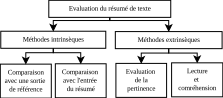
\includegraphics{evalRAT/classif-eval.pdf} % % %[width=140mm]
 \caption{Les approches d'évaluation des systèmes de résumé automatique.}
 \label{fig:classif-eval}
\end{center}
\end{figure}

\subsection{Évaluation intrinsèque}

\subsubsection{Critères utilisés}

Dans le but d'évaluer le résumé produit d'une manière intrinsèque, on compare le résumé produit par rapport au résumé de référence ou carrément avec le document source selon différents critère.
Le premier est la cohérence, qui consiste à la vérification de la lisibilité du résumé. 
Pour les résumés par extraction, les problèmes sont dus à la présence des anaphores et des brèches dans leurs structures rhétoriques. 
Pour les résumés par abstraction, les vérifications qu'on peut faire, d'après \cite{00-saggion-lapalme}, sont: la bonne orthographe et grammaire, l'indication claire sur le document source, style non personnel, la brièveté, la lisibilité et la compréhension, etc. 
Mais jusque-là, il est pratiquement impossible de procéder à une telle évaluation de manière automatique. 

L'autre critère est le contenu informatif du résumé, qui vise à estimer les informations que le résumé contient. 
Comme le résumé est plus court que le texte original, il y a moins d'informations préservées. 
Ainsi, la mesure du contenu informatif d'un résumé consiste à estimer la quantité d'information préservée par rapport au texte source. 

\subsubsection{Comparaison avec une sortie de référence}

L'idée est de comparer le résumé automatique avec celui fait par un humain d'un même texte source. 
L'évaluation classique de \cite{69-edmundson} a été réalisée par humain en comparant le résumé par machine avec celui crée par un humain. 
Le problème pour l'évaluation humain est que, même si on peut trouver plusieurs résumés de référence pour un même document, le système peut générer un résumé qui est différent de tous ces résumés de référence, mais qui est informatif et cohérent \cite{01-mani}. 
Dans une expérience conduite par \cite{61-rath-al}, où on a demandé aux humains d'extraire 20 phrases à partir de 10 articles scientifiques, on a trouvé que les juges ont produit des résumés différents pour la même source. 
En plus, on a trouvé que pour un même juge, celui-ci peut produire deux résumés totalement différents en un intervalle de huit semaines.
On peut aussi évaluer un résumé de manière automatique, en utilisant des différentes mesures, parmi elle ROUGE (va être détaillée ultérieurement).

\subsubsection{Comparaison avec l'entrée de résumé}

Dans ce type d'évaluation, le résumé et la source sont donnés à des personnes, en leurs demandant d'évaluer le contenu informatif du résumé dans le contexte de la source.
Selon \cite{01-mani} il existe deux types de méthodes pour la comparaison entre le résumé et la source: les méthodes sémantiques et les méthodes de surface.
Les méthodes sémantiques consistent à comparer le sens dans le texte source par rapport à celui du résumé. 
Une méthode est de marquer le sens de chaque phrase dans le résumé, ensuite voir combien de propositions existantes dans la source ce résumé couvre. 

Une méthode sémantique plus pratique se trouve dans l'approche de l'extraction d'information de \cite{93-paice-jones}. 
Pour évaluer leur outil de résumé, chaque texte est caractérisé par ses concepts focaux et non focaux. 
Les auteurs ont mesuré la couverture de ces concepts dans un résumé en termes de satisfaisant, non satisfaisant, insuffisant.
Dans les méthodes de surface, on ne cherche pas à représenter les concepts dans un niveau très profond, et donc il suffit de juger si les idées principales dans la source sont couvertes par le résumé. 
Une variante de ce type de méthode a été portée dans TIPSTER SUMMAC \cite{99-mani-al}; une tâche Q\&A (Question and Answer) pour l'évaluation des résumés automatiques. 
Dans cette tâche les passages dans le texte source ont été marqués en se basant sur le critère de pertinence à un sujet. 
Considérant un document et un sujet, un résumé concentré sur un sujet pour ce document est juste lorsqu'il contient des réponses pour les questions qui couvent l'information indispensable dans n'importe quel document jugé pertinent au sujet.

\subsection{Évaluation extrinsèque}

L'idée d'une évaluation extrinsèque d'un résumé est de déterminer l'effet de résumé sur d'autres tâches. 
Il existe plusieurs tâches sur lesquels un résumé peut être appliqué, parmi ces tâches on peut citer celles mentionnées dans \cite{01-mani}:
\begin{itemize}
\item Si le résumé affecte le comportement d'autres tâches, il est possible de mesurer l'efficacité en exécutant ces tâches. 
Par exemple, si on a un système de décision qui se base sur notre système de résumé automatique, on peut mesurer l'efficacité de notre système de résumé en examinant son effet sur le système de décision.
\item On peut examiner l'utilité de résumé avec respect des informations de besoin ou d'objectif, comme trouver des documents pertinentes au besoin d'une personne issus d'une large collection.
\item On peut évaluer l'impact d'un résumé sur le système qu'il le contient, par exemple, comment un outil de résumé peut aider dans un système de question-réponse?
\end{itemize}

\subsubsection{Évaluation de la pertinence}

Dans l'évaluation de la pertinence, on présente à une personne un document et un thème, et on lui demande de déterminer le rapport entre le document et le thème. 
L'influence de résumé sur la justesse et le temps dans la tâche est donc étudiée. 
Malgré que l'évaluation SUMMAC inclue une évaluation Q\&A intrinsèque, son principal attention est sur une évaluation extrinsèque. 
En utilisant un document (qui peut être un résumé ou un texte normal, l'évaluateur ne sais pas apriori sa nature), et une description d'un thème, l'évaluateur humain est amené à juger de la pertinence du document par rapport au thème. 
Il doit, donc, choisir une seule catégorie depuis cinq catégories (chacune a une description avec) qui exprime le thème de document, ou non en choisissant "\textit{aucune catégorie}". 

\subsubsection{Lecture et compréhension}

Dans la tâche de lecture et compréhension, l'évaluateur humain lit d'abord les sources et/ou les résumés assemblés d'un ou plusieurs documents. Il répond sur un test de choix multiples sur le contenu des documents. 
Ensuite, le système calcule le pourcentage des réponses correctes. 
De ce fait, une compréhension humaine basée sur un résumé peut être objectivement comparée avec celle basée sur la source. 
Le raisonnement est donc: si la lecture d'un résumé permet à une personne de répondre à des questions comme s'il a lu la source, le résumé est très informatif.

\section{Mesures intrinsèques populaires}

Les mesures varient selon le type de méthode utilisée: intrinsèque ou extrinsèque. 
La figure \ref{fig:intrin-mesures}, représente les mesures intrinsèques les plus utilisés dans le résumé automatique de texte. 
%
\begin{figure}[ht]
\begin{center}
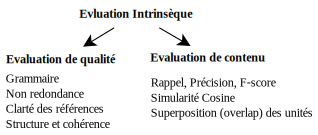
\includegraphics{evalRAT/intrin-mesures.pdf} % % %[width=140mm]
 \caption{Les mesures populaires dans l'évaluation intrinsèque.}
 \label{fig:intrin-mesures}
\end{center}
\end{figure}

\subsection{Évaluation de qualité}

Pour vérifier la qualité (linguistique) d'un texte, il existe des divers aspects:
\begin{itemize}
\item Grammaire: Il faut que le texte soit correct grammaticalement.
\item Non redondance: pas d'information redondante.
\item Clarté des références: Il faut que les liens anaphoriques (relation entre les noms et les pronoms) soient corrects.
\item Structure et cohérence: Le résumé doit avoir une bonne structure avec des phrases cohérentes.
\end{itemize}
Pour attribuer un score à chacun de ces scores, on utilise des évaluateurs humains.
La note peut être, par exemple, un caractère entre A (très bien) et E (très mauvais).

\subsection{Évaluation du contenu}

\subsubsection{Rappel, précision, et F-score}

C'est les mesures les plus utilisées pour juger la performance d'un système de la recherche d'information \cite{08-manning-al} et résumé automatique en particulier. 
Si nous avons un système du résumé automatique qui prend texte d'entrée ($E$), et produit un résumé comme sortie ($S$), et si nous avons un résumé de référence comme modèle ($M$), les relations entre ces documents sont comme suite:
\begin{itemize}
\item TP (true positive): qui est l'information jugée pertinente par $M$ et $S$, donc $M \cap S$.
\item TN (true negative): qui est l'information jugée non pertinente par $M$ et $S$, donc $E - (M \cup S)$.
\item FP (false positive): qui est l'information jugée pertinente par $M$ et non pertinente par $S$, donc $M - S$.
\item FN (false negative): qui est l'information jugée non pertinente par $M$ et pertinente par $S$, donc $S - M$.
\end{itemize}
La figure \ref{fig:mesures} représente ces différentes relations.
%
\begin{figure}[ht]
\begin{center}
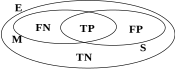
\includegraphics{evalRAT/mesures.pdf} % % %[width=140mm]
 \caption{La relation entre les documents d'entrée, de sortie, et modèle.}
 \label{fig:mesures}
\end{center}
\end{figure}

Le rappel ($R$) représente le pourcentage des éléments pertinents sélectionnés par le système. 
Il est calculé en divisant le nombre des unités communes entre le résultat du système et le résultat attendu, par le nombre des unités composant le résultat attendu. 
Les unités peuvent être des phrases, des mots, etc. 
En utilisant les deux concepts $TP$ et $FN$, on peut exprimer le rappel comme dans l'équation \ref{eq:recall}.
\begin{equation}
\label{eq:recall}
R = \frac {TP} {TP + FN}
\end{equation}

La précision ($P$) représente le pourcentage des éléments sélectionnés qui sont corrects. 
Il est calculé en divisant le nombre des unités communes entre le résultat du système et le résultat attendu, par le nombre des unités composant le résultat du système. 
Les unités peuvent être des phrases, des mots, etc. 
En utilisant les deux concepts $TP$ et $FP$, on peut exprimer le rappel comme dans l'équation \ref{eq:precision}.
\begin{equation}
\label{eq:precision}
P = \frac {TP} {TP + FP}
\end{equation}

Le F-score est un mesure qui combine la précision et le rappel. 
Il est calculé en utilisant une moyenne harmonique entre la précision et le rappel, il est représenté par l'équation \ref{eq:f-score}.
\begin{equation}
\label{eq:f-score}
F_{\beta} = \frac
{(1+\beta^2) P \times R}
{ \beta^2 P + R}
\end{equation}
Le F-score le plus utilisé est le $F_1-score$ en remplaçant $\beta$ par $1$ ce qui nous donne une moyenne harmonique équilibre entre la précision et le rappel.
Lorsque $\beta > 1$, on va favoriser la précision, et lorsque $\beta < 1$ on va favoriser le rappel.

\subsubsection{Similarité de Cosinus}

La similarité cosinus permet de calculer la similarité entre deux vecteurs en déterminant l'angle entre eux. 
L'équation \ref{eq:cosine3} donne la méthode de calcul de similarité Cosinus.
\begin{equation}
\label{eq:cosine3}
cos(X,Y) = 
\frac {X . Y}{||X|| . ||Y||} = 
\frac {\sum_i {x_i.y_i} }{\sqrt{\sum_i(x_i)^2} . \sqrt{\sum_i(y_i)^2}}
\end{equation}
Où: 
X et Y sont deux vecteurs représentant une unité (texte, paragraphe, phrase, mot) du résumé de système et une unité du résumé de référence.

Dans le cas de recherche d'information, la similarité Cosinus de deux documents va être entre 0 et 1, puisqu'on utilise les fréquences des termes qui ne peuvent pas être négatives. 
Donc, l'angle entre deux vecteurs des fréquences des termes va être entre 0\textdegree et 90\textdegree. 
Plus l'angle entre deux vecteurs est petit, plus ils sont similaires. 

%\subsubsection{Superposition (overlap) des unités}
%
%\begin{equation}
%\label{eq:overlap}
%overlap(X,Y) = \frac {||X \cap Y||}
%{||X|| + ||Y|| - ||X \cap Y||}
%\end{equation}

\section{Méthodes d'évaluation}

\subsection{ROUGE}

ROUGE\footnote{ROUGE: Recall-Oriented Understudy for Gisting Evaluation} développé par \cite{03-Lin-hovy} est une méthode inspirée d'une autre méthode d'évaluation des systèmes de traduction automatique, appelée BLEU\footnote{BLEU: BiLingual Evaluation Understudy} \cite{02-papineni-al}. 
L'objectif est de déterminer automatiquement la qualité d'un résumé en le comparant par un autre résumé de référence créé par un humain. 
Le principe est de compter le nombre des unités de recouvrement comme les n-grammes, les séquences de mots, et les mots assemblés entre un résumé généré par ordinateur et le résumé de référence. 
La méthode ROUGE est une méthode basée sur le mesure de rappel puisque le dénominateur est le nombre des n-grammes contenant dans le résumé de référence, par contre la méthode BLEU utilise la mesure de la précision.
La méthode ROUGE contient cinq variantes \cite{04-lin}: ROUGE-N, ROUGE-L, ROUGE-W, ROUGE-S, et ROUGE-SU. 

\subsubsection{ROUGE-N}

ROUGE-N, formellement, est un rappel de n-grammes entre le résumé candidat et un ensemble de résumés de référence. 
La valeur de ROUGE-N peut être calculée par l'équation \ref{eq:rouge-n}. 
\begin{equation}
\label{eq:rouge-n}
ROUGE-(N) = \frac{\sum_{S \in Summ_{ref}}{\sum_{N-gram \in S}{Count_{match} (N-gram)}}}
{\sum_{S \in Summ_{ref}}{\sum_{N-gram \in S}{Count (N-gram)}}}
\end{equation}
Où, \textit{N} est la longueur du N-gramme, $count_{match}(N-gram)$ est le nombre des N-grammes du résumé candidat retrouvées dans un des résumés de référence ($Summ_{ref}$).
$Count (N-gram)$ est le nombre des N-grammes dans le résumé de référence. 

\subsubsection{ROUGE-L}

ROUGE-L utilise la sous-séquence commune la plus longue (LCS\footnote{LCS: Longest Common Subsequence}) entre deux phrases $ X $ avec $m_x$ mots et $ Y $ avec $n_y$ mots, pour estimer la similarité entre ces deux phrases (voir l'équation \ref{eq:lcs}). 
Pour appliquer LCS dans l'évaluation du résumé, il faut voir les phrases de ce résumé comme une séquence de mots. 
Sachant que la séquence commune la plus longue (LCS) ne suppose pas l'appariement consécutif entre les deux séquences. 
\begin{equation}
\label{eq:lcs}
R_{lcs}= \frac {\sum_{i=1}^u {LCS(X, Y)}}{m_x}, 
P_{lcs}= \frac {\sum_{i=1}^u {LCS(X, Y)}}{n_y}
\end{equation}
Pour comprendre mieux comment calculer ROUGE-L, voici un exemple d'une phrase de référence (r1) et deux phrases candidates (c1, c2):
\begin{description}
\item[r1] [\textit{A B C D}].
\item[c1] [\underline{A} E \underline{C D}].
\item[c2] [\underline{C D} E A].
\item[c3] [\underline{C D} \underline{\textit{A B}}].
\end{description}
ROUGE-L de c1 va être 3/4, et de c2 va être 2/4. 
Donc c1 est mieux que c2 selon ROUGE-L. 
Le problème de ROUGE-L est qu'elle calcule seulement la séquence principale, et donc autres LCS alternatifs ou moins longs ne vont pas être considérés dans le calcul du score. 
Dans la phrase c3, LCS compte seulement une séquence et pas les deux, et donc la valeur de ROUGE-L de c3 va être égale à celui de c2.

L'équation \ref{eq:rouge-l} représente la méthode de calcul de ROUGE-L (rappel et précision) entre un résumé de référence $r_i \in R$ et un résumé candidat $C$. 
\begin{equation}
\label{eq:rouge-l}
R_{lcs}= \frac {\sum_{i=1}^u {LCS_{\cup}(r_i, C)}}{m}, 
P_{lcs}= \frac {\sum_{i=1}^u {LCS_{\cup}(r_i, C)}}{n}
\end{equation}
Où:
\begin{itemize}
\item $u$ est le nombre des phrases dans le résumé de référence $R$. 
\item $LCS_{\cup}(r_i, C)$ est le score LCS de l'union des plus longues séquences entre la phrase de référence $r_i$ et les phrases du résumé candidat $C$. Par exemple:
\begin{quote}
Supposant une phrase de référence $r_i = w_1 w_2 w_3 w_4 w_5$, et $C$ contient deux phrases: $c_1 = w_1 w_2 w_6 w_7 w_8$ et $c2 = w_1 w_3 w_8 w_9 w_5$. 
Donc, le LCS entre $r_i$ et $c_1$ est "$w_1 w_2$", et le LCS entre $r_i$ et $c_2$ est "$w_1 w_3 w_5$";
L'union de ces deux LCS nous donne "$w_1 w_2 w_3 w_5$" et $LCS_{\cup}(r_i, C)= 4/5$.
\end{quote}
\item $m$ est le nombre des mots dans $R$, et $n$ est le nombre des mots dans $C$. 
\end{itemize}

\subsubsection{ROUGE-W}

Malgré les bonnes propriétés du LCS notées auparavant, il souffre du problème de différenciation entre les sous-séquences communes ayant des différentes relations spatiales dans leurs séquences originales.
Par exemple, si on a une séquence de référence r1 et deux séquences candidates c1 et c2 comme suit:
\begin{description}
\item[r1] [\underline{A} \underline{B} \underline{C} \underline{D} E F G]
\item[c1] [\underline{A} \underline{B} \underline{C} \underline{D} H I K]
\item[c2] [\underline{A} H \underline{B} K \underline{C} I \underline{D}]
\end{description}
c1 et c2 ont le même score ROUGE-L, mais dans ce cas c1 devrait avoir un score supérieure à celui de c2, puisqu'elle contient des appariements consécutifs. 
Pour améliorer la méthode de LCS, les appariements consécutifs sont accordés plus de score que les appariements non consécutifs. 
Ceci est accompli en pénalisant toute séquence non consécutive. 

L'équation \ref{eq:rouge-w} représente la méthode de calcul de ROUGE-W (rappel et précision) entre un résumé de référence $r_i \in R$ et un résumé candidat $C$. 
\begin{equation}
\label{eq:rouge-w}
R_{wlcs}= f^{-1}(\frac {WLCS(r_i,C)}{f(m)}), 
P_{wlcs}= f^{-1}(\frac {WLCS(r_i,C)}{f(n)})
\end{equation}
Où:
\begin{itemize}
\item $ f $ est une fonction satisfaisant la relation $ f(x,y)>f(x)+f(y) $. Prenant $ f(k) = k^2 $ où $ k $ est la taille d'une LCS.
\item $WLCS(r_i,C) = \sum_j f(LCS_j(r_i,C))$, $LCS_j(r_i,C)$ est la taille de LCS numéro $ j $ entre la phrase de référence $r_i$ et les phrases du résumé candidat $C$. Par exemple:
\begin{quote}
Dans l'exemple précédent, c1 donne une seule LCS: "A B C D". 
Donc, $ ROUGE-W(c1) = \sqrt{(4^2)}/7 = 0.57143 $. 

Pour la deuxième séquence c2, on a quatre LCS: "A", "B", "C", et "D". 
Donc, $ ROUGE-W(c2) = \sqrt{(1^2 + 1^2 + 1^2 + 1^2)}/7 = 0.28571 $. 
\end{quote}
\item $m$ est le nombre des mots dans $R$, et $n$ est le nombre des mots dans $C$. 
\end{itemize}

\subsubsection{ROUGE-S}

ROUGE-S\footnote{ROUGE-S: skip-bigram co-occurrence} est une extension de ROUGE-N; elle est calculée de la même manière que ROUGE-2, sauf qu'elle utilise les bi-grammes à trous au lieu des bi-grammes consécutives. 
Le bi-gramme à trous (skip bigram), comme défini dans \cite{04-lin}, est n'importe quelle paire de mots dans leurs ordre dans la phrase, qui permettent des trous arbitraires. 
Si on a $X$ un texte de référence avec $m$ mots et $Y$ un texte candidat avec $n$ mots, on peut calculer ROUGE-S comme suit.
\begin{equation}
\label{eq:rouge-s}
R_{SKIP2}(X, Y) = \frac {SKIP2(X, Y)}{C(m, 2)}, 
P_{SKIP2}(X, Y) = \frac {SKIP2(X, Y)}{C(n, 2)}
\end{equation}
Où $SKIP2(X,Y)$ est le nombre des bi-grammes à trous semblables entre $X$ et $Y$.
$C$ est la fonction de combinaison.

Prenant l'exemple utilisé dans ROUGE-L, où r1 est la phrase de référence et les trois phrases c1, c2, et c3 sont les phrases candidates: 
\begin{description}
\item[r1] [\textit{A B C D}].
\item[c1] [A E C D].
\item[c2] [C D E A].
\item[c3] [C D A B].
\end{description}
Chaque phrase contient $C(4,2)=6$ bi-grammes à trous. 
Par exemple la phrase c1 a les bi-grammes suivants: ("A E", "A C", "A D", "E C", "E D", "C D"). 
Le score ROUGE-S pour c1, c2, et c3 sont: 3/6, 1/6, et 2/6 respectivement.

\subsubsection{ROUGE-SU}

Un problème de ROUGE-S est qu'elle ne donne aucun crédit pour une phrase candidate si cette phrase ne contient aucune paire de mots semblables à ceux de la phrase de référence.
Par exemple, la phrase suivante donne un score ROUGE-S à zéro:
\begin{description}
\item[c4] [D C B A].
\end{description}
Cette phrase est l'inverse de la phrase r1 et il n'existe aucun bi-gramme à trous similaire à ceux de r1. 
Pourtant, on veut faire la différence entre les phrases comme c4 et les phrases qui ne contiennent aucun mot en commun avec r1. 
Pour le faire, on peut étendre ROUGE-S avec l'addition des uni-grammes comme unités de calcule, ce qui nous donne ROUGE-SU.

Chaque phrase contient $C(4,2) + 4 = 10$ grammes. 
Par exemple la phrase c1 a les grammes suivants: ("A E", "A C", "A D", "E C", "E D", "C D", "A", "B", "C", "D"). 
Le score ROUGE-SU pour c1, c2, c3, et c4 sont: 7/10, 5/10, 6/10, et 4/10 respectivement.

\subsection{BE}

%Définir les BEs
Les éléments basiques (\textit{Basic Elements: BEs}) sont des unités sémantiques minimales qu'on peut obtenir d'une phrase. 
D'après \cite{06-hovy-al}, le problème d'évaluation du contenu d'un résumé peut être résolu en utilisant trois différents modules: découpeur de BE, comparateur de BE , et évaluateur de BE. 
Le premier sert à créer les unités BE d'un texte d'entrée, le deuxième sert à évaluer la similarité entre deux BE, et le troisième sert à donner un score pour chaque BE.

Le système d'évaluation utilisant les BEs prend le résumé et un ensemble des résumés de référence pour avoir un score. 
Il applique les trois modules précédents deux fois, en deux étapes: la préparation et la notation. 
Dans la phase de préparation, le premier module décompose les résumés de référence en une liste de BEs de référence; le second module prend en compte tous BEs de référence et fusionne ceux sémantiquement identiques et le troisième module attribue un score à chacun des BEs de référence.
Dans la deuxième étape (notation), le premier module décompose le résumé en une liste séparée de BEs, le second compare chaque BE à la liste des BEs de référence, le troisième attribue un score à chaque BE et calcule le score global de tous les BEs contenus dans le résumé candidat.

Le découpeur de BE est consacré pour décomposer un texte sur des BEs, en utilisant une des règles de découpage construites manuellement exécutées sur l'arbre syntaxique du texte d'entrée. 
Des expérimentations sont conduites par \cite{06-hovy-al} pour définir les BEs comme suit:
\begin{itemize}
\item l'entête d'un constituant syntaxique majeur (nom, verbe, adjectif, ou phrase adverbiale) exprimé comme un élément seul, ou
\item une relation entre un BE d'entête et un dépendant simple, exprimé comme un triple (entête, modificateur, relation).
\end{itemize}

%comparaison des BEs
Le comparateur sert à comparer deux BEs en utilisant des stratégies de comparaison. 
Les stratégies de comparaison sont catégorisées sur plusieurs classes (de la plus simple à la plus complexe):
\begin{itemize}
\item Similitude lexicale: les mots doivent être comparables exactement.
\item Similitude de lemmes: les formes racines des mots doivent être comparables.
\item Similitude de synonyme: les mots ou leurs synonymes identifiés par WordNet, doivent être comparables exactement.
\item Les paraphrases doivent être comparables (une approximation).
\item La généralisation sémantique: les mots construisant les BEs sont remplacés par leurs généralisations sémantiques ("Peugeot" sera remplacé par "voiture") puis comparés dans une diversité des niveaux d'abstraction.
\end{itemize}

%Donner un score pour les BEs
L'évaluateur sert à donner un score à chaque BE. 
Dans \cite{06-hovy-al}, les auteurs ont attribué à chaque BE un (1) point à chaque fois qu'il participe à un résumé de référence. 
Ce score est attribué en se basant sur la similarité entre le BE et les BEs de référence.
Le score global est la somme des poids des BEs qui figurent dans le résumé candidat.

\subsection{Pyramides}

L'évaluation de similarité entre le résumé automatique et le résumé humain, se fait en utilisant des métriques comme la précision et le rappel. 
Mais, selon \cite{07-nenkova-al}, cette méthode présente quelques inconvénients: 
\begin{itemize}
\item La variation humaine: différentes personnes peuvent sélectionner des phrases différentes à intégrer dans le résumé. 
Même pour une personne, elle peut produire deux résumés différents. 

\item Granularité de l'analyse: Même si le système ne choisit pas exactement la même phrase que le résumé modèle, cette phrase peut être pertinente avec une ou plus de phrases du modèle. 
L'appariement partiel doit être pris en compte, mais il exige une analyse au-dessous du niveau phrase. 

\item L'équivalence sémantique: différentes phrases peuvent exprimer la même signification, même si elles n'utilisent pas les mêmes mots. 
Naturellement, les annotateurs doivent choisir seulement une phrase parmi les phrases équivalentes, et le système qui choisit une autre phrase équivalente doit être pénalisé. 

\item Extrait ou abstrait? Le résumé humain est un résumé par abstraction; une personne utilise ses propres mots pour rédiger un résumé. 
Ainsi, l'appariement exact entre les phrases de système et celle du modèle (fait par l'humain) n'est pas possible. 
\end{itemize}

La méthode Pyramides \cite{07-nenkova-al}, a été développée dont l'objectif est de remédier à ces problèmes.
Elle est une évaluation quantitative du contenu sélectionné par un système de résumé, qui nécessite un résumé de référence qu'on puisse utiliser pour évaluer le résumé généré automatiquement.
La pyramide est une représentation du résumé de référence attribué à chaque ensemble de documents d'entrée. 
Puisque le pyramide est utilisé pour évaluer le contenu du résumé, les unités de comparaison dans un pyramide correspondent aux unités de signification (sens), il sont appelées "\textit{summary content units (SCUs)}". 

Contrairement aux méthodes utilisant un résumé de référence, un pyramide représente les opinions de plusieurs résumeurs humains, qui ont écrit chacun un résumé modèle pour l'ensemble de documents d'entrée. 
La caractéristique clé d'un pyramide est qu'il quantifie l'accord entre les résumés humains. 
Les SCUs qui apparaissent dans plus de résumés humains vont avoir plus de score, ce qui nous permet de faire la différence entre le contenu plus important que celui moins important. 

Une fois l'annotation faite, les SCUs finaux sont partitionnés sur un pyramide en se basant sur les poids de ces SCUs. 
Chaque étage contient seulement les SCUs ayant le même poids. 
Le nombre \textit{n} des résumés modèles annotés, représente le nombre maximal d'étages dans un pyramide. 
La taille d'un pyramide (nombre d'étages) peut être différent de sa taille dans le cas où il n'y a pas une superposition entre tous les modèles utilisés dans la création de pyramide. 
Il y a un petit nombre de SCUs (dans la sommet de pyramide), que tout le monde ont exprimé dans leurs résumés, et un trop large nombre de SCUs exprimés par un seul résumé modèle (dans la base de pyramide). 
Donc, en descendant dans le pyramide, les SCUs deviennent moins importants dans leurs informations, vu qu'ils apparaissent dans moins de résumés. 
La figure \ref{fig:meth-pyramids} représente un pyramide avec deux SCUs dans le sommet et quatre dans l'étage suivant, elle illustre deux  parmi six résumés optimaux de taille 4 SCUs que ce pyramide prévoit. 
\begin{figure}[ht]
\begin{center}
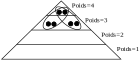
\includegraphics{evalRAT/meth-pyramids.pdf} % % %[width=140mm]
 \caption[Deux parmi six résumés optimaux avec 4SCU]{Deux parmi six résumés optimaux avec 4SCU \cite{07-nenkova-al}.}
 \label{fig:meth-pyramids}
\end{center}
\end{figure}

En se basant sur une pyramide, le contenu informatif du nouveau résumé peut être calculé comme le rapport entre la somme des poids de ses SCUs et le poids d'un résumé optimal avec le même nombre de SCUs. 
%\cite{07-nenkova-al} ont présenté une formule pour calculer le poids de résumé optimal (voir la formule \ref{eq:max-pyramids}). 
%\begin{equation}
%\label{eq:max-pyramids}
%Max = \sum_{i=j+1}^{n}{i\times |T_i|+j \times (X - \sum_{i=j+1}^{n}{|T_i|})} ; 
%j= \max_i{(\sum_{t=i}^{n}{|T_t|\geq X})}
%\end{equation}
%Où $n$ est le nombre des étage dans le pyramide, 
%$T_i$ est l'étage numéro $i$ (Le poids des SCUs dans l'étage $T_i$ égale à $i$), 
%$|T_i|$ est le nombre des SCUs dans l'étage $i$, 
%et $X$ est la taille du résumé en SCUs. 

\section{Campagnes d'évaluation}

\subsection{SUMMAC}

SUMMAC est la première conférence d'évaluation de résumé automatique\cite{99-mani-al}, elle est lancée par le gouvernement Américain en mai 1998. 
Trois tâches principales d'évaluation ont été définies: la tâche ad-hoc, la tâche de catégorisation, et la tâche question-réponse. 

Dans la tâche ad-hoc, le centre d'intérêt est les résumés indicatifs adaptés à un thème particulier. 
Pour un document (qui peut être un résumé ou un texte source, l'évaluateur ne sait pas), et une description d'un thème, on demande à l'évaluateur de déterminer si le document est pertinent pour le thème. 

Dans la tâche de catégorisation, l'évaluation cherche à trouver si un résumé générique peut aider un analyste de catégoriser un document rapidement et correctement. 
Ici, le thème n'est pas connu pour le système de résumé. 
Pour un document, qui peut être un résumé générique ou un texte source (l'évaluateur ne sait pas), le testeur doit choisir parmi cinq catégories données, celle pour laquelle le document est pertinent, sinon il choisit "\textit{aucune catégorie}". 

La tâche question-réponse implique l'évaluation du contenu informatif du résumé par rapport à un thème donné; c'est-à-dire le nombre de réponses qu'on peut trouver, en lisant le résumé, pour des questions reliées à ce thème et générées du document source. 
Chaque résumé est comparé manuellement à la réponse de référence pour un document donné, pour juger si la réponse de résumé est correcte, partiellement correcte, ou incorrecte.
Deux métriques d'exactitude sont utilisés: ARS (\textit{Answer Recall Strict}) et ARL (\textit{Answer Recall Lenient}), représentés par l'équation \ref{eq:answer-recall}.
\begin{equation}
\label{eq:answer-recall}
ARS = \frac{n1}{n3}, 
ARL = \frac{n1 + (.5 * n2)}{n3}
\end{equation}
Où $ n1 $ est le nombre des réponses correctes dans le résumé, $ n2 $ est le nombre des réponses partiellement correctes, et $ n3 $ est le nombre des questions répondues dans la réponse de référence.

\subsection{DUC/TAC}

DUC\footnote{DUC site web: \url{http://duc.nist.gov/}} (Document Understanding Conference) est une série d'évaluations organisée par NIST\footnote{NIST: National Institute of Standards and Technology} dans le cadre du projet TIDES\footnote{TIDES: DARPA's Translingual Information Detection, Extraction, and Summarization.}. 
Il a comme but de faire évaluer la technologie des résumés automatique en permettant aux chercheurs de participer à des expériences à grande échelle. 
Dans DUC 2004, il y avait 5 tâches d'évaluation:
\begin{itemize}

\item \textbf{La tâche 1 - résumés très courts mono-document:} Pour chaque document des 50 documents en Anglais, il faut créer un résumé très court (<=75 octets).

\item \textbf{La tâche 2 - résumés courts multi-document:} Pour chaque groupe des 50 groupes de documents en Anglais, il faut créer un résumé court (<=665 octets).

\item \textbf{La tâche 3 - résumés très courts mono-document trans-linguistique:} Pour chaque translation en Anglais (automatique et manuelle) des 25 documents en Arabe, il faut créer un résumé très court (<=75 octets).

\item \textbf{La tâche 4 - résumés courts multi-document trans-linguistique:} Pour chaque groupe de translations en Anglais (automatique et manuelle) des 25 groupes de documents en Arabe, il faut créer un résumé court (<=665 octets).

\item \textbf{La tâche 5 - résumés courts guidés par une requête:} Pour chaque groupe des 50 groupes de documents en Anglais, il faut créer un résumé court (<=665 octets) pour répondre à une question au forme "\textit{Who is X?}", où X est le nom d'une personne ou groupe de personnes.

\end{itemize}
Les résumés qui dépassent la taille limite vont être tronqués, et aucun bonus ne va être attribué aux résumés plus courts. 
L'évaluation des tâches 1-4 est faite en utilisant ROUGE (ROUGE-1, ROUGE-2, ROUGE-3, ROUGE-4, et ROUGE-L). 
Pour la tâche 5, les résumés sont évalués, d'une façon intrinsèque, en terme de qualité et de couverture en utilisant le système SEE\footnote{SEE: Summary Evaluation Environment (\url{http://www.isi.edu/licensed-sw/see/})}. 
En terme de pertinence vis-à-vis la question "\textit{Who is X?}", ils sont évalués par des évaluateurs humains.

Dans DUC 2007, les documents utilisés pour le résumé sont ceux du corpus AQUAINT, contenant des articles hebdomadaire diversifiés de \textit{Associated Press} et \textit{New York Times} (1998-2000) et \textit{Xinhua News Agency} (1996-2000).
Il y avait 2 tâches: tâche principale et tâche de mise-à-jour.
\begin{itemize}
\item \textbf{Tâche principale:} En fournissant 25 documents et un thème, la tâche est de synthétiser un résumé courant et bien organisé de 200 mots afin de répondre à une ou plusieurs questions. 

\item \textbf{Tâche de mise-à-jour:} le but est de produire des résumés courts multi-documents (environ 100 mots) de mise-à-jour en supposant que l'utilisateur a déjà lu l'ensemble des articles précédents.
\end{itemize}
Pour la première tâche, l'évaluation est conduite comme suit:
\begin{itemize}
\item la forme linguistique est évaluée manuellement pour chaque résumé, en utilisant des critères de qualité: la grammaire, la non redondance, la clarté de références, la concentration, la structure et la cohérence. 
Pour chacun de ces critères, les évaluateurs donnent une note entre 1 (pas bon) et 5 (très bon). 

\item La pertinence vis-à-vis un thème donné, est évaluée manuellement pour chaque résumé en utilisant une note entre 1 (pas bon) et 5 (très bon).

\item Pour chaque résumé automatique, ROUGE-2 et ROUGE-SU4 sont calculés.

\item Pour chaque résumé automatique, BE est calculé.
\end{itemize}
Pour la deuxième tâche, chaque résumé va être évalué selon: ROUGE-2, ROUGE-SU4, BE, et Pyramides.

Depuis 2008, DUC a été inclus dans la conférence TAC comme une tâche nommée "le résumé guidé". 
La tâche de résumé guidé (\textit{guided summarization}) a comme but d'encourager les systèmes de résumé de faire une analyse linguistique (sémantique) plus profonde sur les documents sources que d'utiliser les fréquences de mots pour sélectionner les concepts. 
Dans TAC 2010, la tâche de résumé guidé est de générer un résumé de 100 mots pour un ensemble de 10 articles de presse pour un thème donné, où le thème appartient à une catégorie prédéfinie. 
Il y a cinq catégories des thèmes: les accidents et les catastrophes naturelles, les crises, la santé et de la sécurité, les ressources menacées, les enquêtes et les procès.
Pour un thème donné, la tâche est d'écrire 2 résumés (pour deux ensembles de documents A et B):
\begin{itemize}
\item Un résumé pour l'ensemble A est guidé par requête.
\item Un résumé guidé par requête pour l'ensemble B sachant que l'utilisateur du résumé a déjà lis les documents de l'ensemble A.
\end{itemize}
Chaque résumé doit couvrir des aspects définis pour son catégorie (par exemple, WHAT? WHY? WHEN? WHERE?). 
L'évaluation se fait sur le contenu, la lisibilité, et la sensibilité. 
Pour le contenu, le score est calculé par la méthode Pyramides. 
Pour la lisibilité et la sensibilité globale, des évaluateurs sont demandés de donner un score entre 1 (très mauvais) et 5 (très bon).

\subsection{NTCIR}

L'atelier NTCIR est une série d'évaluations désignée pour supporter la recherche dans les technologies d'accès à l'information, y compris la recherche d'information, les questions-réponses, le résumé de texte, l'extraction, etc. 
L'objectif de NTCIR est: 
\begin{enumerate}
\item D'encourager la recherche dans les technologies d'accès à l'information en fournissant des collections de test large-échelle utilisées pour les expériences et les évaluations. 
\item De fournir un forum pour les groupes de recherche qui s'intéressent à la comparaison entre systèmes et l'échange d'idées. 
\item D'examiner les méthodes d'évaluation des techniques d'accès d'information et les méthodes de construction de corpus de données large-échelle utilisées dans les expériences. 
\end{enumerate}

Dans le deuxième atelier de NTCIR (1999), le défi de résumé automatique de textes contient trois tâches. 
Les deux premières tâches sont pour l'évaluation intrinsèque (appelés tâche A) où les participants résument automatiquement des documents en spécifiant la longueur de résumé. 
La troisième tâche est pour l'évaluation extrinsèque (appelé tâche B) où les résumés sont évalués en conduisant une tâche de RI. 
Les processus de ces tâches sont comme suit \cite{01-fukusima-okumura}:
\begin{itemize}
\item \textbf{Tâche A-1:} dans cette tâche le but est d'extraire les phrases les plus importantes. 
Le taux de résumé est défini comme la proportion entre le nombre des phrases choisies et le nombre total des phrases dans l'article. 
Les taux utilisés dans cette tâche sont 10\%, 30\%, 50\%.

\item \textbf{Tâche A-2:} dans cette tâche le but est de produire des résumés (par abstraction) en simple texte pour être comparés avec les résumés préparés par les humains. 
Le taux de résumé est défini comme la proportion entre le nombre des caractères dans le résumé et le nombre total des caractères dans l'article. 
Les taux utilisés dans cette tâche sont environ 20\% et 40\%. 

\item \textbf{Tâche B:} dans cette tâche le but est de produire des résumés en se basant sur des requêtes et des documents trouvés selon ces requêtes. 
Pour chacun de ces documents, il faut produire un résumé (pas un résumé multi-documents). 
La longueur du résumé n'est pas limitée, mais les résumés doivent être en un texte simple (sans marquages HTML, XML, etc.). 
\end{itemize}

Pour les documents utilisés, des experts sont demandés de sélectionner les phrases les plus importantes dans chaque document source pour évaluer les résumés par extraction. 
Pour les résumés par abstraction, le résumé produit manuellement en utilisant deux manières; la première est de sélectionner les parties importantes dans les phrases extraites manuellement, la deuxième est de résumé le document librement. 
L'évaluation des tâche se fait comme suit \cite{01-fukusima-okumura}:
\begin{itemize}
\item \textbf{Tâche A-1:} On cherche les phrases correctes dans le résumé.
Ensuite, on calcule les métriques: rappel, précision, et f1-score pour chaque résumé en prenant le nombre des phrases comme unité de calcule pour ces métriques. 
Le score final est la moyenne des scores de tous les résumés. 

\item \textbf{Tâche A-2:} Dans cette tâche, l'évaluation se fait selon deux manières: l'évaluation basée sur le contenu et l'évaluation subjective. 
Dans la première évaluation, les résumés système ainsi que les deux types de résumé humains sont analysés morphologiquement pour extraire des vecteurs contenant les mots de contenu, ensuite la distance entre le vecteur des fréquences de mots de résumé humain et de système est calculée. 
Dans la deuxième évaluation, on demande des juges humains d'évaluer les résumés selon deux critères la couverture et la lisibilité, en donnant une note entre 1 (très bien) et 4 (très mauvais). 
Les juges disposent de 4 résumés: les deux résumés humains, le résumé système, et un résumé produit en se basant sur la méthode LEAD. 

\item \textbf{Tâche B:} Dans cette tâche, les évaluateurs disposent des requêtes et des résumés des documents trouvés selon ces requêtes. 
Ils lisent les résumés et jugent la pertinence de ces documents vis-à-vis la requête. 
La méthode d'évaluation est essentiellement la même que celle de SUMMAC. 
Les mesures rappel, précision, et f1-score sont utilisés en prenant le nombre des documents comme unité pour ces mesures, ainsi que le temps nécessaire pour cette tâche. 
\end{itemize}

\section{Défis de l'évaluation} 

Selon Mani \cite{01-mani}, il existe plusieurs défis quant à l'évaluation des résumés automatiques:
\begin{itemize}
\item Le résumé implique une sortie produite par machine qui résulte dans la communication par langage naturel. 
Dans le cas où la sortie est une réponse à une question, il existe peut-être une réponse correcte, mais dans d'autres cas il est difficile d'arriver à définir c'est quoi une sortie correcte.
Il y a toujours la possibilité qu'un système génère un bon résumé qui soit tout-à-fait différent des résumés humains utilisés pour l'évaluation. 

\item Étant donné que c'est à un humain de juger de la sortie du système, ceci peut diminuer considérablement les charges d'une évaluation. 
Une évaluation utilisant un programme de score au lieu de jugements humains est préférable, puisque on peut la répéter facilement. 

\item Le résumé entraîne la compression, donc il est important d'évaluer les résumés dans des différents taux de compression. 
Ceci augmente l'échelle et la complexité d'une évaluation. 
Puisque le résumé implique la présentation de l'information adapté aux besoins des utilisateurs, la prise en compte de ces facteurs complique d'avantage le processus d'évaluation. 
\end{itemize}

\section{Conclusion}

Dans ce chapitre, nous avons présenté un état de l'art sur l'évaluation de résumé automatique. 
L'évaluation de résumé automatique et plus généralement les systèmes RI est un domaine de recherche eu lui-même, qui ne peut être décrit dans un chapitre. 
Dans un premier temps, nous avons défini les deux approches d'évaluation de résumé automatique: l'évaluation intrinsèque et l'évaluation extrinsèque. 
Pour évaluer un résumé, des mesures sont utilisés, parmi ces mesures nous avons cité les plus utilisés dans l'évaluation intrinsèque. 
Ces mesures évaluent la qualité linguistique de résumé, ainsi que le contenu informatif du résumé. 
Parmi les méthodes utilisées pour l'évaluation intrinsèque, nous avons cité: ROUGE, BE, et Pyramides, utilisés dans différentes campagnes d'évaluation: DUC/TAC, SUMMAC, et NTCIR. 
Finalement, nous avons mis les points sur les défis qui rendent l'évaluation à une tâche difficile à faire. 

%Dans le chapitre suivant
Dans le chapitre suivant, nous allons présenter notre système de résumé automatique basé sur l'approche statistique. 
L'idée principale est d'améliorer cette approche en introduisant le regroupement pour trouver les différents thèmes présents dans le document source. 
Ensuite en utilisant un algorithme d'apprentissage, nous avons créé un modèle pour chaque thème. 
En utilisant ces modèles, on cherche à trouver les phrases qui peuvent représenter tous (ou la plupart) des thèmes. 

%========================Le pied de chapitre=======================================
%==================================================================================
\ifx\wholebook\relax\else
 \cleardoublepage
 \bibliographystyle{../use/ESIbib} %../includes/ThesisStyle
 \bibliography{../bib/evalRAT} %,../bib/yay
 \end{document}
\fi
%==================================================================================

\clearpage

\part{Résumé automatique par regroupement et apprentissage sans corpus d'entraînement} %Notre contribution

%==================================================================================
%==================================================================================
% Document		:		Chapitre: Méthode proposée pour le résumé automatique de textes
%
% Auteur		: 		Abdelkrime ARIES
% Encadreur		:		Dr. Omar NOUALI
% Co-encadreur	:		Mme. Houda OUFAIDA
% Établissement	:		ESI (Ecole Nationale Supérieure d'Informatique; ex. INI) 
% Adresse		:		Oued Smar, Alger, Algérie 
% Année			:		2012/2013
% Grade			:		Magister
% discipline 	:		Informatique 
% Spécialité	:		IRM (Informatique Répartie et Mobile)
% Titre			:		Résumé automatique de textes
%
%==================================================================================
%==================================================================================

%==========================L'entete de chapitre====================================
%==================================================================================
 \ifx\wholebook\relax\else
  	\documentclass[a4paper,12pt,oneside]{../use/ESIthesis}
  	
  	\usepackage{amsmath,amssymb}             % AMS Math
\usepackage[utf8]{inputenc}
%\usepackage[T1]{fontenc} %,LAE 
\usepackage[T1]{fontenc}
%\usepackage[french,english]{babel}
\usepackage[frenchb]{babel}
\usepackage{microtype}

%\usepackage[left=2.5cm,right=2.5cm,top=2.5cm,bottom=2.5cm,includefoot,includehead,headheight=13.6pt]{geometry}
\usepackage[left=2.8cm,right=2.2cm,top=2.8cm,bottom=2.8cm,includefoot,includehead,headheight=13.6pt]{geometry}
%\usepackage[left=3.8cm,right=3.2cm,top=2.8cm,bottom=2.8cm,includefoot,includehead,headheight=13.6pt]{geometry}
%\usepackage[left=1.5in,right=1.3in,top=1.1in,bottom=1.1in,includefoot,includehead,headheight=13.6pt]{geometry}
\renewcommand{\baselinestretch}{1.5}

% Table of contents for each chapter

\usepackage[nottoc, notlof, notlot]{tocbibind}
\usepackage[french]{minitoc}
\setcounter{minitocdepth}{1}
\mtcindent=15pt
% Use \minitoc where to put a table of contents

\usepackage{aecompl}

% Glossary / list of abbreviations

\usepackage[intoc]{nomencl}
%\renewcommand{\nomname}{List of Abbreviations}

\makenomenclature

% My pdf code

\usepackage[pdftex]{graphicx}
\usepackage[a4paper,pagebackref,hyperindex=true]{hyperref}

%I added
%\usepackage{tabulary}
%\usepackage{longtable}
%\usepackage[table]{xcolor}
\usepackage{indentfirst}


% Links in pdf
\usepackage{color}
%\definecolor{linkcol}{rgb}{0,0,0.4} 
%\definecolor{citecol}{rgb}{0.5,0,0} 

% Change this to change the informations included in the pdf file

% See hyperref documentation for information on those parameters

\hypersetup
{
%bookmarksopen=true,
pdftitle=Résumé Automatique de Textes,
pdfauthor=Abdelkrime ARIES, 
pdfsubject= {Résumé automatique de textes en utilisant une approche statistique, le regroupement, et la classification} , %subject of the document
%%pdftoolbar=false, % toolbar hidden
%pdfmenubar=true, %menubar shown
%pdfhighlight=/O, %effect of clicking on a link
colorlinks=false, %couleurs sur les liens hypertextes
%pdfpagemode=None, %aucun mode de page
%pdfpagelayout=SinglePage, %ouverture en simple page
%pdffitwindow=true, %pages ouvertes entierement dans toute la fenetre
%linkcolor=linkcol, %couleur des liens hypertextes internes
%citecolor=citecol, %couleur des liens pour les citations
%urlcolor=linkcol %couleur des liens pour les url
}



% Some useful commands and shortcut for maths:  partial derivative and stuff

\newcommand{\pd}[2]{\frac{\partial #1}{\partial #2}}
\def\abs{\operatorname{abs}}
\def\argmax{\operatornamewithlimits{arg\,max}}
\def\argmin{\operatornamewithlimits{arg\,min}}
\def\diag{\operatorname{Diag}}
\newcommand{\eqRef}[1]{(\ref{#1})}

\usepackage{rotating}                    % Sideways of figures & tables
%\usepackage{bibunits}
%\usepackage[sectionbib]{chapterbib}          % Cross-reference package (Natural BiB)
%\usepackage{natbib}                  % Put References at the end of each chapter
                                         % Do not put 'sectionbib' option here.
                                         % Sectionbib option in 'natbib' will do.
\usepackage{fancyhdr}                    % Fancy Header and Footer

\usepackage{txfonts}                     % Public Times New Roman text & math font
  
%%% Fancy Header %%%%%%%%%%%%%%%%%%%%%%%%%%%%%%%%%%%%%%%%%%%%%%%%%%%%%%%%%%%%%%%%%%
% Fancy Header Style Options

\pagestyle{fancy}                       % Sets fancy header and footer
\fancyfoot{}                            % Delete current footer settings

%\renewcommand{\chaptermark}[1]{         % Lower Case Chapter marker style
%  \markboth{\chaptername\ \thechapter.\ #1}}{}} %

%\renewcommand{\sectionmark}[1]{         % Lower case Section marker style
%  \markright{\thesection.\ #1}}         %
%\fancyhead[LE,RO]{\bfseries\thepage}    % Page number (boldface) in left on even
%										% pages and right on odd pages
%\fancyhead[RE]{\bfseries\nouppercase{\leftmark}}      % Chapter in the right on even pages
%\fancyhead[LO]{\bfseries\nouppercase{\rightmark}}     % Section in the left on odd pages

\fancyhead[R]{\bfseries\thepage}    % Page number (boldface) in right
\fancyhead[L]{\bfseries\nouppercase{\rightmark}}     % Section in the left on odd pages

\let\headruleORIG\headrule
\renewcommand{\headrule}{\color{black} \headruleORIG}
\renewcommand{\headrulewidth}{1.0pt}
\usepackage{colortbl}
\arrayrulecolor{black}

\fancypagestyle{plain}{
  \fancyhead{}
  \fancyfoot{}
  \renewcommand{\headrulewidth}{0pt}
}

%\usepackage{algorithm}
%\usepackage[noend]{algorithmic}

%%% Clear Header %%%%%%%%%%%%%%%%%%%%%%%%%%%%%%%%%%%%%%%%%%%%%%%%%%%%%%%%%%%%%%%%%%
% Clear Header Style on the Last Empty Odd pages
\makeatletter

\def\cleardoublepage{\clearpage\if@twoside \ifodd\c@page\else%
  \hbox{}%
  \thispagestyle{empty}%              % Empty header styles
  \newpage%
  \if@twocolumn\hbox{}\newpage\fi\fi\fi}

\makeatother
 
%%%%%%%%%%%%%%%%%%%%%%%%%%%%%%%%%%%%%%%%%%%%%%%%%%%%%%%%%%%%%%%%%%%%%%%%%%%%%%% 
% Prints your review date and 'Draft Version' (From Josullvn, CS, CMU)
\newcommand{\reviewtimetoday}[2]{\special{!userdict begin
    /bop-hook{gsave 20 710 translate 45 rotate 0.8 setgray
      /Times-Roman findfont 12 scalefont setfont 0 0   moveto (#1) show
      0 -12 moveto (#2) show grestore}def end}}
% You can turn on or off this option.
% \reviewtimetoday{\today}{Draft Version}
%%%%%%%%%%%%%%%%%%%%%%%%%%%%%%%%%%%%%%%%%%%%%%%%%%%%%%%%%%%%%%%%%%%%%%%%%%%%%%% 

\newenvironment{maxime}[1]
{
\vspace*{0cm}
\hfill
\begin{minipage}{0.5\textwidth}%
%\rule[0.5ex]{\textwidth}{0.1mm}\\%
\hrulefill $\:$ {\bf #1}\\
%\vspace*{-0.25cm}
\it 
}%
{%

\hrulefill
\vspace*{0.5cm}%
\end{minipage}
}

\let\minitocORIG\minitoc
\renewcommand{\minitoc}{\minitocORIG \vspace{1.5em}} %1.5em

\usepackage{multirow}
%\usepackage{slashbox}

\newenvironment{bulletList}%
{ \begin{list}%
	{$\bullet$}%
	{\setlength{\labelwidth}{25pt}%
	 \setlength{\leftmargin}{30pt}%
	 \setlength{\itemsep}{\parsep}}}%
{ \end{list} }

\newtheorem{definition}{Définition }
\renewcommand{\epsilon}{\varepsilon}

% centered page environment

\newenvironment{vcenterpage}
{\newpage\vspace*{\fill}\thispagestyle{empty}\renewcommand{\headrulewidth}{0pt}}
{\vspace*{\fill}}

%%%%%%%%%%%%%%%%%%%%%%%%%%%%%%%%%%%%%%%%%%%%%%%%%%%%%%%%%%%%%%%%%%%%
% Par Karim
%%%%%%%%%%%%%%%%%%%%%%%%%%%%%%%%%%%%%%%%%%%%%%%%%%%%%%%%%%%%%%%%%%%%
%for the degree sign
\usepackage{textcomp} 
\usepackage{bookmark}
\usepackage{framed}
\usepackage{arabtex}
%\usepackage{nashbf}
%\usepackage{atrans}
%calligra font for the remerciement
\usepackage{calligra}

%List of acronyms
\usepackage{acronym}

\newcommand{\racine}{./}

\newcommand{\setracine}[1]{\renewcommand{\racine}{#1}}

\newcommand{\tablefile}[1]{\input{\racine tab/#1}}
\newcommand{\appendixfile}[1]{\input{\racine anx/#1}}
%\newcommand{\chapterfile}[1]{\input{\racine chap/#1}}

\newcommand{\stitle}[1]{
\noindent
\textbf{#1}
}

\newenvironment{itemizeb}
{\begin{list}{\textbullet} {\setlength{\rightmargin}{0cm} \setlength{\leftmargin}{1cm}}}
{\end{list}}


\newenvironment{itemizec}
{\begin{list}{\textopenbullet} {\setlength{\rightmargin}{0cm} \setlength{\leftmargin}{1cm}}}
{\end{list}}


\newcommand{\kexpbox}[1]{

\vspace{5mm}
\noindent
 \fbox{%
   \parbox{0.985\linewidth}{%
   \vspace{2mm}
   {\large  \textbf{Exemple:}}\\
      #1
   }%
 }
}

\newcommand{\kbox}[1]{

\vspace{2mm}
\noindent
 \fbox{%
   \parbox{0.965\linewidth}{%
   \vspace{2mm}
      #1
   }%
 }
}

\newenvironment{kexp}
{
\begin{framed}
\noindent
{\large  \textbf{Exemple:}}\\
}
{
\end{framed}
}

%%%%%%%%%%%%%%%%%%%%%%%%%%%%%%%%%%%%%%%%%%%%%%%%%%%%%%%%%%%%%%%%%%%%
%%%%%%%%%%%%%%%%%%%%%%%%%%%%%%%%%%%%%%%%%%%%%%%%%%%%%%%%%%%%%%%%%%%%

% definitions.
% -------------------

\setcounter{secnumdepth}{3}
\setcounter{tocdepth}{2}

\newcommand{\tab}[1]{{\hskip #1}}
  	 	
  	 	\setracine{../}
  	 	\graphicspath{{.}{../fig/}}
  	 	
  	 	\begin{document}
  	 	
  	 	\dominitoc 
  	 	\selectlanguage {francais}
  	 	%just to create the .toc file, then you can hide it
  	 	%\tableofcontents
  	 	\mainmatter
  \fi
%==================================================================================

\chapter{Méthode proposée pour le résumé automatique de textes}
\label{chap:mine}
\minitoc

\section{Introduction}

Après avoir vu les différents travaux sur le résumé automatique, en mettant l'accent sur les méthodes statistiques. 
Celles-ci sont des méthodes simples, faciles à manipuler, et rapides si on les compare aux méthodes linguistiques. 
En effet, elles utilisent peu de ressources linguistiques (dans la phase de pré-traitement en général), ceci les rend peu dépendant de la langue. 
Cependant, il existe des manques dont on essaye de couvrir en utilisant plus de ressources linguistiques. 
Dans notre approche, nous proposons d'utiliser conjointement la classification et le regroupement sur la base de critères de type numérique afin de produire des résumés génériques indépendamment du genre ou de la langue.

En premier lieu, nous allons présenter l'architecture générale de notre système, pour pouvoir spécifier exactement notre contribution par rapport à cette architecture. 
Puisque notre méthode se base sur le regroupement, nous allons présenter cette tâche, afin de décrire le procédé de délétion des différents thèmes de document, ainsi que la tâche de classification. 
Dans notre travail, la classification ne se base sur aucun corpus d'entraînement, elle est utilisée pour trouver un modèle pour chaque cluster, pour ensuite noter les phrases suivant ces modèles. 
Enfin, nous allons présenter l'application de notre méthode sur le résumé multi-documents.

\section{Architecture générale}

Les systèmes de résumé automatiques, statistiques, linguistiques, ou hybrides ont tous besoins d'une phase de pré-traitement pour rendre le texte d'entrée conforme à la phase de traitement. 
Ils utilisent, ainsi, un module de post-traitement qui s'occupe, généralement, de la présentation du résumé au lecteur. 
En examinant les systèmes de résumé automatique, on peut dire que le module de traitement est celui qui définit la différence entre tous ces systèmes. 
Notre système ne fait pas l'exception par rapport aux autres systèmes de résumé automatique, il comporte aussi les trois modules classiques qui sont le pré-traitement, le traitement, et le post-traitement (voir la figure \ref{fig:gnrl-arch}). 
%
\begin{figure}[ht]
\begin{center}
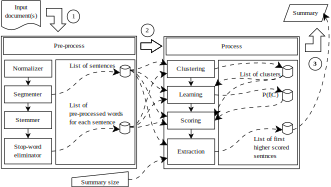
\includegraphics{mine/gnrl-arch.pdf}
\caption{L'architecture générale de notre système.}
\label{fig:gnrl-arch}
\end{center}
\end{figure}

Pour mieux comprendre la méthode, nous allons utiliser un texte qui va être utilisé dans tous les modules. 

\begin{kexp}
Supposant que notre texte d'entrée est composé des cinq phrases suivantes:
\begin{enumerate}
\item \textit{My name is Karim, and I study informatics at ESI, which is at Algiers, to obtain Magister degree.}
\item \textit{My research in ESI is about ATS, it is the intersection between IR and NLP.}
\item \textit{In this research, the main idea is to find relevant sentences using IR technics.}
\item \textit{The statistical features are the power of IR to find relevancy.}
\item \textit{AI technics are used, such as learning algorithms to create models for each topic in the input text.}
\end{enumerate}
\end{kexp}

\subsection{Module de pré-traitement}

Dans le module de pré-traitement, on nécessite les étapes suivantes:
\begin{itemize}
\item Segmentation des phrases en utilisant le framework OpenNLP d'Appache\footnote{Site web: \url{http://opennlp.apache.org/}}. 
\item Pour détecter les mots, on a implémenté un simple algorithme est utilisé, qui prend l'espace comme caractère de séparation. 
\item Pour la radicalisation, nous avons utilisé Porter-stemmer \footnote{\url{http://www.tartarus.org/~martin/PorterStemmer}}; une implémentation de l'algorithme de Porter \cite{97-porter} en Java.
\end{itemize}

\begin{kexp}
Le pré-traitement de l'exemple précédent donne:
\begin{enumerate}
\item \textit{karim studi informat esi algier obtain magist degre} (8 termes)
\item \textit{research esi at intersect ir nlp} (6 termes)
\item \textit{research main idea find relev sentenc ir technic} (8 termes)
\item \textit{statist featur power ir find relev} (6 termes)
\item \textit{ai technic learn algorithm creat model topic input text} (9 termes)
\end{enumerate}
\end{kexp}
%\subsection{Module de traitement}
%
%Ce module représente le le cœur d notre système, il permet d'extraire les phrases les plus pertinentes sous forme réduite.
%Ainsi, il comporte deux sous-modules: un module de réduction de phrases, et un module d'extraction. 

\subsection{Module d'extraction}

Le module d'extraction est le module le plus important dans notre système. 
Il contient la méthode proposée pour l'extraction de phrases, en essayant de maximiser la couverture des thèmes pris en charge. 
Elle contient deux étapes: l'étape d'identification des thèmes abordés dans le document, et l'étape de classification. 
Pour détecter les différents thèmes présentés dans le document, nous avons utilisé le regroupement, ici on assume que les phrases contenant des mots similaires sont des phrases de même thème. 
Dans l'étape de classification, on essaye de concevoir un modèle de chaque groupe (cluster), qui va être utilisé pour calculer la probabilité qu'une phrase appartient à un thème donné.

\subsubsection{Notre motivation}

Dans les méthodes qui utilisent le regroupement \cite{01-nomoto-al,02-hardy-al,11-song-al}, chaque thème fournit une phrase qui le représente dans le résumé; i.e. on sélectionne une phrase par thème. 
Dans ces travaux, assurer la couverture de tous les thèmes par le résumé produit pose un problème de contrôle de la taille du résumé. 
En effet, pour un résumé de 10 documents, par exemple, avec 50 thèmes identifiés et si on sélectionne une phrase associée à chaque cluster, on aura donc un résumé de 50 phrases, ce qui n'est pas du tout pratique. 
%Les thèmes négligeables par rapport au thème principal, sont souvent ignorés par ces travaux.
Le problème avec ces méthodes est que, pour tout thème identifié, on extrait une phrase correspondante malgré que, naturellement, tous les thèmes n'ont la même importance et il y en a même quelques thèmes qui sont négligeables. 
On peut trouver aussi des thèmes qui ne peuvent pas être représentés ou résumé par une seule phrase. 

L'idée principale est de sélectionner les phrases qui peuvent représenter tous ou la plupart des thèmes, en donnant à une phrase un score pour, ensuite, combiner ces scores en un score final utilisé pour l'ordonnancement des phrases.
Afin de calculer le score de chaque phrase par thème, on utilise un algorithme d'apprentissage (Naïve Bayes), pour entrainer le système sur les différents clusters et les critères. 
Contrairement aux systèmes précédents basés sur l'apprentissage \cite{95-kupiec-al,01-amini-gallinari,02-osborne,05-yeh-al,10-yatsko-al}, ce système n'a pas besoin d'un corpus d'entraînement, l'apprentissage est utilisé uniquement pour l'obtention du score par cluster. 

\subsubsection{Le regroupement}

Afin de regrouper les phrases, nous avons utilisé une mesure de calcul de la similarité entre deux segments : la similarité Cosinus. Cette mesure a été largement appliquée dans le domaine de la recherche d'information.
Ici, l'équation \ref{eq:cosine-g} est utilisé pour calculer la similarité Cosinus entre deux phrases $ X $ et $ Y $.
\begin{equation}
\label{eq:cosine-g}
cos(X,Y) = \frac {\sum_i {x_i.y_i} }
{\sqrt{\sum_i(x_i)^2} . \sqrt{\sum_i(y_i)^2}}
\end{equation}
Où: $ x_i $ est le mot numéro $ i $ dans la phrase $ X $, et $ y_i $ est le mot numéro $ i $ dans la phrase $ Y $.
Pour notre exemple, les deux phrases $ s_3 $ et $ s_4 $ ont les termes \{ir, find, relev\} en commun. 
Donc, $ cos(s_3,s_4)= (1*1 + 1*1 + 1*1) /(\sqrt{1^2+1^2+1^2+1^2+1^2+1^2+1^2+1^2}*\sqrt{1^2+1^2+1^2+1^2+1^2})\approx 0.43$.

Ainsi, on considère que deux phrases $ X $ et $ Y $ sont similaires, si leur similarité cosinus $ cos(X,Y) $ est supérieure à un certain seuil $ Th $.
Notre algorithme de regroupement passe par les étapes suivantes (voir la figure \ref{fig:cluster}):
\begin{figure}[ht]
\begin{center}
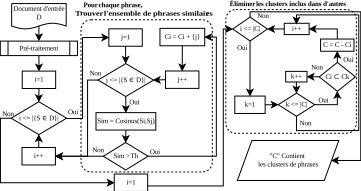
\includegraphics[width=160mm]{mine/cluster.pdf}
\caption{Algorithme de regroupement.}
\label{fig:cluster}
\end{center}
\end{figure}
\begin{itemize}
\item Pour chaque phrase, on calcule sa similarité avec toutes les autres phrases en utilisant l'équation \ref{eq:cosine-g}.

\item Ensuite, on utilise un seuil $ Th $ pour sélectionner les phrases les plus similaires. 
Si le seuil est élevé, les clusters formés vont contenir un nombre réduit de phrases. 
S'il est trop faible, les clusters seront, serte, moins nombreux et plus grands, mais en contrepartie on perd en termes de cohésion des clusters, les thèmes deviennent ainsi flous. %\cite{Clustering-Hardy-2002}

\item Chaque phrase et celles qui lui sont similaires vont construire un cluster. 

\item Nous exécutons les trois premières étapes jusqu'à ce qu'il ne reste aucune phrase. 

\item Après avoir terminé toutes les $ n $ phrases, nous obtenons $ n $ clusters (une phrase peut appartenir à plusieurs clusters). 

\item Pour chaque cluster, on vérifie s'il n'est pas inclut dans un autre cluster. Sinon, on l'efface. 

\item Enfin, on obtient un nombre total de clusters inférieur ou égal au nombre de phrases.

\end{itemize}

\begin{kexp}
Prenant notre exemple précédent, en suivant les étapes de notre algorithme, on aura:
\begin{itemize}
\item Les similarités entre les cinq phrases sont: $ cos(s_1,s_2) \approx 0.14$, $ cos(s_1,s_3) = cos(s_1,s_4) = cos(s_1,s_5) =0.0 $, $ cos(s_2,s_3) \approx 0.29 $, $ cos(s_2,s_4) \approx 0.17 $, $ cos(s_2,s_5) =0.0 $, $ cos(s_3,s_4) \approx 0.43 $, $ cos(s_3,s_5) \approx 0.12 $, et $ cos(s_4,s_5) \approx 0.0 $.

\item Prenant la valeur $ Th=0.2 $.

\item On aura les clusters suivants: $ C_1 = \{s_1\} $, $ C_2 = \{s_2, s_3\} $, $ C_3 = \{s_2, s_3, s_4\} $, $ C_4 = \{s_3, s_4\} $, $ C_5 = \{s_5\} $.

\item On remarque que le cluster $ C_2 $ est inclus dans le cluster $ C_3 $, et le cluster $ C_4 $ est inclus dans le cluster $ C_3 $.

\item Après suppression et ré-ordonnancement de clusters, on aura $ C_1 = \{s_1\} $, $ C_2 = \{s_2, s_3, s_4\} $, $ C_3 = \{s_5\} $.

\end{itemize}
\end{kexp}

\subsubsection{La fonction de score en utilisant la classification}

Dans le but de rendre notre méthode aussi générale que possible, nous avons choisi de ne pas utiliser un corpus d'apprentissage, et plutôt, nous utilisons différents clusters pour le faire.
Supposant que nous avons des clusters de phrases similaires. 
Dans notre méthode, nous voulons trouver les phrases qui sont les plus probables pour représenter tous les clusters. 
Ceci peut être représenté par l'équation suivante: 
\begin{equation}
\label{eq:sent-score}
P(s_i \in \bigcap_{j} C_j | \overrightarrow{f}) = 
\prod_{j} P(s_i \in C_j | \overrightarrow{f})
\end{equation}
Où $s_i$ est la phrase numéro $i$, $C_j$ est la classe $j$, et $\overrightarrow{f}$ est le vecteur de critères (fréquence de mots, longueur de phrase, position de phrase, etc.).

Pour calculer la probabilité qu'une phrase $s_i$ appartient à une classe $C_j$ sachant un vecteur de critères $\overrightarrow{f}$, nous avons utilisé la classification de Bayes. 
Si nous supposons l'indépendance de critères et, en utilisant la théorème de Bayes, nous avons:
\begin{equation}
\label{eq:bayes}
P(s_i \in C_j | \overrightarrow{f}) = 
\frac{P(s_i \in C_j) . P(\overrightarrow{f} | s_i \in C_j) }{P(\overrightarrow{f})}
\end{equation}
Puisque le dénominateur ne dépend pas des classes et les valeurs des critères (constant), l'équation \ref{eq:bayes} s'écrit:
\begin{equation}
\label{eq:bayes2}
P(s_i \in C_j | \overrightarrow{f}) \propto 
P(s_i \in C_j) . P(\overrightarrow{f} | s_i \in C_j)
\end{equation}
De l'équation \ref{eq:sent-score} et \ref{eq:bayes2}, on obtient l'équation suivante:
\begin{equation}
\label{eq:bayes3}
P(s_i \in \bigcap_{j} C_j | \overrightarrow{f}) \propto 
\prod_{j} P(\overrightarrow{f} | s_i \in C_j)
\end{equation}
Car nous multiplions toutes les probabilités a priori ($P(s_i \in C_j)$), le résultat peut être supprimée puisqu'elle est constante. 
En revanche, Bayes suppose l'indépendance de critères les uns des autres, et donc l'équation \ref{eq:bayes3} peut être écrite comme suit:
\begin{equation}
\label{eq:bayes4}
P(s_i \in \bigcap_{j} C_j | \overrightarrow{f}) \propto 
\prod_{j} \prod_{k} P(f_k | s_i \in C_j)
\end{equation}

Pour faciliter la combinaison des différents critères d'une phrase, en particulier ceux de la fréquence du terme, nous proposons d'utiliser un score plutôt qu'une probabilité. 
Un autre raison est que la classification utilisée ici n'est qu'un outil de score (donner des scores à une phrase dans chaque cluster), et pas la construction d'un modèle qui permet de définir les phrases de résumé ou de régler les poids des critères. 
Alors, l'équation \ref{eq:bayes4} va être écrite comme suit:
\begin{equation}
\label{eq:class-score}
Score(s_i , \bigcap_{j} C_j , \overrightarrow{f}) = 
\prod_{j} \prod_{k} Score(s_i , C_j , f_k )
\end{equation}
Enfin, les phrases vont être réorganisées selon leurs scores. 
La fonction $ Score( s , C , f ) $ est utilisée pour calculer le score de la phrase $ s $ dans la classe $ C $, en utilisant le critère $ f $ qui peut apparaître plusieurs fois dans cette phrase. 

Ensuite, on passe à l'échelle de logarithme, et la formule \ref{eq:class-score} devienne:
\begin{equation}
\label{eq:log-class-score}
Score_{log}(s_i , \bigcap_{j} C_j , \overrightarrow{f}) = 
\sum_{j} \sum_{k} log (Score(s_i , C_j , f_k ))
\end{equation}
Il est à noter que l'application du logarithme ne change pas l'ordre des scores, elle nous permet seulement de réduire l'espace des valeurs.

\subsubsection{L'apprentissage}

Pendant la tâche d'apprentissage, la probabilité qu'un critère apparaît dans une classe est donnée par l'équation \ref{eq:likelihood}.
Où $\phi$ est l'observation de le critère $ f $ dans la classe $ C $. 
$F_{C\phi}$ est le nombre d'apparition de $\phi$ dans la classe $ C $.
\begin{equation}
\label{eq:likelihood}
P(f = \phi | C) = \frac {F_{C\phi}}{\sum_{\phi'}{F_{C\phi'}}}
\end{equation}
et ainsi,
\begin{equation}
\label{eq:sum_likelihood}
\sum_{\phi} P(f = \phi | C) = 1
\end{equation}
Le score d'une phrase $ s $ dans une classe $ C $ en utilisant un critère $ f $,peut être représenté comme la somme des probabilités des observations de $ f $.
Ensuite, on ajoute un à la somme pour éviter la multiplication par un score d'un critère égal à zéro.
\begin{equation}
\label{eq:score}
Score(s , C , f ) = 1 + \sum_{\phi \in s} {P(f=\phi | s \in C)}
\end{equation}

\begin{kexp}
Dans notre exemple, nous allons utiliser les deux critères: les uni-grammes et les bi-grammes. 
Les statistiques de chaque cluster (ou class) seront:
\begin{itemize}
\item $\mathbf{C_1 = \{s_1\}} $:\\
\textbf{uni}=\{degre=1, magist=1, algier=1, obtain=1, informat=1, karim=1, esi=1, studi=1\}.\\
\textbf{bi}=\{informat?esi=1, karim?studi=1, >>?karim=1, magist?degre=1, studi?informat=1, algier?obtain=1, obtain?magist=1, esi?algier=1\}.

\item $ \mathbf{C_2 = \{s_2, s_3, s_4\}} $:\\
\textbf{uni}=\{ir=3, idea=1, technic=1, relev=2, esi=1, at=1, research=2, statist=1, main=1, sentenc=1, featur=1, power=1, nlp=1, itersect=1, find=2\}.\\
\textbf{bi}=\{idea?find=1, find?relev=2, itersect?ir=1, power?ir=1, ir?nlp=1, main?idea=1, >>?research=2, research?esi=1, sentenc?ir=1, research?main=1, featur?power=1, >>?statist=1, esi?at=1, ir?technic=1, relev?sentenc=1, at?itersect=1, statist?featur=1, ir?find=1\}.\\

\item $ \mathbf{C_3 = \{s_5\}} $:\\
\textbf{uni}=\{topic=1, text=1, input=1, model=1, ai=1, technic=1, creat=1, learn=1, algorithm=1\}.\\
\textbf{bi}=\{input?text=1, technic?learn=1, creat?model=1, algorithm?creat=1, >>?ai=1, model?topic=1, topic?input=1, learn?algorithm=1, ai?technic=1\}.
\end{itemize}

Maintenant, calculons la probabilité de l'occurrence "ir" de critère "uni-grammes" dans le deuxième cluster $ P(f = "ir" | C_2) $. 
$ P(f = "ir" | C_2) = 3/(3+1+1+2+1+1+2+1+1+1+1+1+1+1+2) = 3/20 = 0.15$. 
Pour simplifier le calcul, et puisque le nombre des occurrences de critères dans les clusters vont être multiplié qui nous donne un nombre constant, nous allons prendre $ P(f = "ir" | C_2) = 3 $.

pour chaque phrase, on calcule son score dans un cluster $ C $ avec un critère $ f $ en utilisant l'équation \ref{eq:score}. 
Le score de la phrase $ s_3 $ dans le cluster $ C_2 $ avec le critère "uni-grammes" sera: 
$ Score(s_3 , C_2 , uni ) = 1 + (2 + 1 + 1 + 2 + 2 + 1 + 3 + 1) = 14 $. 
De même, on aura:
\begin{enumerate}
\item $ Score(s_1 , C_1 , uni ) = 9 $, $ Score(s_1 , C_1 , bi ) = 9 $, 
$ Score(s_1 , C_2 , uni ) = 2 $, $ Score(s_1 , C_2 , bi ) = 1 $, 
$ Score(s_1 , C_3 , uni ) = 1 $, $ Score(s_1 , C_3 , bi ) = 1 $.

\item $ Score(s_2 , C_1 , uni ) = 2 $, $ Score(s_2 , C_1 , bi ) = 1 $, 
$ Score(s_2 , C_2 , uni ) = 10 $, $ Score(s_2 , C_2 , bi ) = 8 $, 
$ Score(s_2 , C_3 , uni ) = 1 $, $ Score(s_2 , C_3 , bi ) = 1 $.

\item $ Score(s_3 , C_1 , uni ) = 1 $, $ Score(s_3 , C_1 , bi ) = 1 $, 
$ Score(s_3 , C_2 , uni ) = 14 $, $ Score(s_3 , C_2 , bi ) = 11 $, 
$ Score(s_3 , C_3 , uni ) = 2 $, $ Score(s_3 , C_3 , bi ) = 1 $.

\item $ Score(s_4 , C_1 , uni ) = 1 $, $ Score(s_4 , C_1 , bi ) = 1 $, 
$ Score(s_4 , C_2 , uni ) = 11 $, $ Score(s_4 , C_2 , bi ) = 8 $, 
$ Score(s_4 , C_3 , uni ) = 1 $, $ Score(s_4 , C_3 , bi ) = 1 $.

\item $ Score(s_5 , C_1 , uni ) = 1 $, $ Score(s_5 , C_1 , bi ) = 1 $, 
$ Score(s_5 , C_2 , uni ) = 2 $, $ Score(s_5 , C_2 , bi ) = 1 $, 
$ Score(s_5 , C_3 , uni ) = 10 $, $ Score(s_5 , C_3 , bi ) = 10 $.

\end{enumerate}

En utilisant l'équation \ref{eq:log-class-score} et ces scores, on peut calculer le score total de chaque phrase. 
Pour chaque phrase, on aura les scores suivants: $ Score(s_1) \approx 5.09 $, $ Score(s_2) \approx 5.08 $, $ Score(s_3) \approx 5.73 $, $ Score(s_4) \approx 4.48 $, $ Score(s_5) \approx 5.30 $.
\end{kexp}

\subsubsection{La normalisation}

En utilisant le score dans l'équation \ref{eq:class-score}, les phrases dont la taille est petite, sont toujours défavorisées, et donc n'ont pas une grande chance contre celles de grande taille. 
En plus, en utilisant la réduction de phrases et en comparant les phrases réduites avec celles originales, ces dernières sont toujours favorisées.
Pour résoudre ce problème, le score peut être normalisé sur la taille du phrase en nombre de termes. 
L'équation \ref{eq:class-score} va, donc, être écrite comme suite:
\begin{equation}
\label{eq:score-norm}
Score_{norm}(s_i , \bigcap_{j} C_j , \overrightarrow{f}) = 
\frac{1}{|s_i|}
\prod_{j} \prod_{k} Score(s_i , C_j , f_k )
\end{equation}
Où: $ |s_i| $ est le nombre de termes dans la phrase $ s_i $.

En utilisant le logarithme, cette équation peut être écrit comme suit:
\begin{equation}
\label{eq:score-norm-log}
Score_{norm+log}(s_i , \bigcap_{j} C_j , \overrightarrow{f}) = 
Score_{log}(s_i , \bigcap_{j} C_j , \overrightarrow{f}) - log(|s_i|)
\end{equation}
Pour garantir que la longueur $ |s_i| $ ne soit pas à 0, on va ajouter 1. 

\begin{kexp}
Les scores de notre exemple vont être: 
\begin{enumerate}
\item $ Score_{norm}(s_1) = 5.09 - log(9) \approx 2.89 $,
\item  $ Score_{norm}(s_2) = 5.08 - log(7) \approx 3.13 $, 
\item  $ Score_{norm}(s_3) = 5.73 - log(9) \approx 3.53 $, 
\item  $ Score_{norm}(s_4) = 4.48 - log(7) \approx 2.53 $, 
\item  $ Score_{norm}(s_5) = 5.30 - log(10) \approx 3.0 $.
\end{enumerate}
\end{kexp}

\subsection{Module de compression}

%La réduction dans le premier module se fait avant l'extraction. % d'une façon similaire de \cite{07-zajic-al}. 
Pour chaque phrase de texte, on cherche la phrase compressée si elle existe. 
À la fin, nous allons avoir un nombre sa forme compressée inférieur ou égale au nombre de phrases du texte. 
Elles vont ensuite recevoir un score tout comme les phrases originale, mais elles ne participent pas dans les statistiques, puisque leurs phrases originales l'ont déjà fait. 
Dans une première fois, nous avons utilisé un algorithme très primitif pour compresser les phrases, seulement pour voir l'effet de réduction sur les résumés, et si ce chemin mérite d'être suivi ou non.
En voyant d'une façon technique à la réduction de phrases, nous ne supprimons que les expressions d'explication dont la pattern est comme suite:
\begin{itemize}
\item , which [\textasciicircum,]*,
\item , who [\textasciicircum,]*,
\item \_ [\textasciicircum\_]* \_
\end{itemize}

La première phrase "\textit{My name is Karim, and I study informatics at ESI, which is at Algiers, to obtain Magister degree.}" peut être compressée en utilisant cet algorithme, en éliminant le passage "\textit{, which is at Algiers,}". 
Le score normalisé de la phrase compressée sera $ Score(s_{1-reduit}) \approx 2.64 $. 
Dans cet exemple, la réduction n'a pas amélioré le score de la phrase 1.
%La réduction de phrases nous permet d'ajouter d'autres informations au résumé, et d'éliminer l'information non nécessaire. 
%Lorsque nous avons évalué la réduction, nous avons trouvé qu'elle peut améliorer un peu de la qualité de résumé, portant elle est si simple. 
%Cela nous encourage d'utiliser un module plus évolué dans le futur.

\subsection{Module de post-traitement}

Étant donné que notre but est, dans un premier temps, d'améliorer la qualité en termes contenu informationnel du résumé résultant, et non pas sa représentation, l'ordre des phrases, la résolution des anaphores, et l'enchaînement des idées entre les phrases font partie des perspectives de notre travail.

Concernant le problème de redondance d'information, nous avons utilisé la similarité entre phrases pour éliminer les phrases redondante du résumé. 
Ça nous permet d'avoir plus d'information dans notre résumé. 
Les étapes suivantes décrivent l'algorithme suivi afin d'éliminer la redondance:
\begin{enumerate}
\item Étant donné l'ensemble des phrases ordonnées par leurs scores, ajouter la première phrase au résumé.
\item Pour chaque phrase candidate, on vérifie si le résumé a atteint sa limite.
Si c'est le cas, on s'arrête; Sinon, on continue.
\item On calcule la similarité entre la dernière phrase ajoutée au résumé et la phrase candidate. 
Si la similarité est inférieure à certaine valeur (nous avons utilisé 0.5), on l'ajoute au résumé. 
Sinon, on passe à la phrase suivante. 
\end{enumerate}
%Notre justification est que les phrases similaires vont attribuées presque le même score. 
%C'est pour cette raison, on ne fait la comparaison qu'avec la dernière phrase dans le résumé.

En ce qui concerne la résolution des anaphores, nous avions choisi d'utiliser le module de résolution des anaphores développé par le groupe NLP de l'université de Stanford "Stanford CoreNLP\footnote{Site web: \url{http://nlp.stanford.edu/software/corenlp.shtml}}" \cite{13-lee-al}.
Ce système met en œuvre une méthode de résolution d'anaphores multi-passes décrit dans \cite{11-lee-al} et \cite{10-raghunathan}.
Pour notre cas, on fait passer tous le texte par ce module pour ensuite corriger celles qui sont présente au niveau du résumé.

\section{Application au résumé multi-documents}

\subsubsection{Résumé en utilisant les documents comme clusters}

La première méthode consiste à considérer chaque document en entrée comme un cluster de phrases pour ensuite appliquer l'algorithme d'apprentissage sur chaque document à part. 
En deuxième lieu, chaque modèle est utilisé pour la notation de phrases des documents d'entrée.
La figure \ref{fig:system1} illustre les différentes étapes de cette méthode. 
%
\begin{figure}[!ht]
\begin{center}
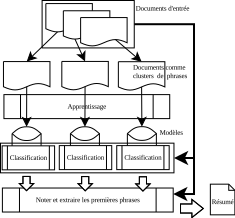
\includegraphics[width=100mm]{mine/system1.pdf} %[width=100mm]
\caption{Architecture du système en utilisant chaque document comme cluster.}
\label{fig:system1}
\end{center}
\end{figure}

Dans cette architecture, chaque cluster est un document d'entrée. 
Le problème est que les documents d'entrée ont le même thème général, et des thèmes secondaires qui peuvent être différents d'un document à l'autre. 
Donc, l'algorithme d'apprentissage va générer des modèles qui sont très proches. 
Cela nous conduit d'utiliser une autre méthode qui nous permet de traiter des clusters plus distinctifs.

\subsubsection{Résumé par fusion de documents}

La deuxième méthode consiste à fusionner tous les documents d'entrée, en les considérant comme un seul document. 
Ainsi, on regroupe les phrases similaires dans le même cluster. 
Ensuite, on applique l'algorithme d'apprentissage sur les clusters de phrases pour obtenir un modèle pour chacun. 
Finalement, chaque modèle est utilisé pour donner un score pour chaque phrase des documents d'entrée.
La figure \ref{fig:system2} illustre les différentes étapes de cette méthode. 
%
\begin{figure}[!ht]
\begin{center}
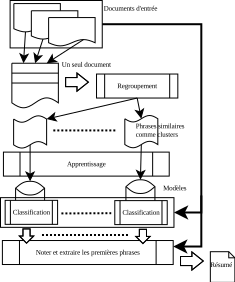
\includegraphics[width=100mm]{mine/system2.pdf} %[width=100mm]
\caption{Architecture du système en fusionnant les documents.}
\label{fig:system2}
\end{center}
\end{figure}

\section{Conclusion}

Dans ce chapitre, nous avons présenté notre système de résumé automatique de textes. 
Premièrement, nous avons présenté l'architecture générale utilisée par les systèmes de résumé automatique, en spécifiant les différents modules, ainsi que la description de chaque module dans notre système.
Le module, au cœur systèmes d'extraction, est le module d'extraction. 
Dans notre système, ce module utilise deux techniques: le regroupement pour trouver les différents thèmes de document(s), et la classification pour donner un score à chaque phrase. 
Ainsi, nous avons présenté l'algorithme de regroupement que nous avons utilisé pour définir des clusters contenant les phrases ayant le même thème. 
Ensuite, nous avons discuté l'utilisation de la classification pour trouver les phrases pertinentes sans avoir besoin d'un corpus d'entraînement. 
Ces deux techniques sont utilisées dans le résumé mono-document, en utilisant les clusters résultants de regroupement comme entrée au système d'apprentissage pour mesurer la pertinence des phrases par rapport à tous les thèmes de texte. 
Nous avons présenté deux approches pour le résumé multi-documents: la première prend chaque document comme cluster de phrases, et la deuxième fusionne les différents documents. 

Notre méthode de regroupement est utilisée pour détecter les différents thèmes de document(s), d'une manière simple et rapide, afin de tester l'effet du regroupement sur le système de résumé. 
On peut utiliser d'autres méthodes de regroupement plus évolués, pour assurer une identification plus précise des différents thèmes de texte. 
En ce qu concerne la classification, nous avons choisi le classificateur Naïve Bayes, qui est simple à modéliser et qui a prouvé son utilité pour le résumé automatique à base d'apprentissage. 
%On peut toujours tester d'autres algorithmes de classification, ce qu'il n'est pas notre but dans ce travail. 

Dans le chapitre suivant, nous allons présenter les différentes évaluations conduites sur notre système. 
Nous allons évaluer l'effet des seuils de regroupement sur le résumé résultant, ainsi que l'effet d'ajout de critères. 
Enfin, on va comparer notre système avec d'autres systèmes de résumé automatique de texte. 

\ifx\wholebook\relax\else
 %\chapterfoot
 \cleardoublepage
 \bibliographystyle{../use/ESIbib} 
 \bibliography{../bib/mine} 
 \end{document}
\fi

\clearpage

%==================================================================================
%==================================================================================
% Document		:		Chapitre: Évaluation de la méthode proposée
%
% Auteur		: 		Abdelkrime ARIES
% Encadreur		:		Dr. Omar NOUALI
% Co-encadreur	:		Mme. Houda OUFAIDA
% Établissement	:		ESI (Ecole Nationale Supérieure d'Informatique; ex. INI) 
% Adresse		:		Oued Smar, Alger, Algérie 
% Année			:		2012/2013
% Grade			:		Magister
% discipline 	:		Informatique 
% Spécialité	:		IRM (Informatique Répartie et Mobile)
% Titre			:		Résumé automatique de textes
%
%==================================================================================
%==================================================================================

%==========================L'entete de chapitre====================================
%==================================================================================
 \ifx\wholebook\relax\else
  	\documentclass[a4paper,12pt,oneside]{../use/ESIthesis}
  	
  	\usepackage{amsmath,amssymb}             % AMS Math
\usepackage[utf8]{inputenc}
%\usepackage[T1]{fontenc} %,LAE 
\usepackage[T1]{fontenc}
%\usepackage[french,english]{babel}
\usepackage[frenchb]{babel}
\usepackage{microtype}

%\usepackage[left=2.5cm,right=2.5cm,top=2.5cm,bottom=2.5cm,includefoot,includehead,headheight=13.6pt]{geometry}
\usepackage[left=2.8cm,right=2.2cm,top=2.8cm,bottom=2.8cm,includefoot,includehead,headheight=13.6pt]{geometry}
%\usepackage[left=3.8cm,right=3.2cm,top=2.8cm,bottom=2.8cm,includefoot,includehead,headheight=13.6pt]{geometry}
%\usepackage[left=1.5in,right=1.3in,top=1.1in,bottom=1.1in,includefoot,includehead,headheight=13.6pt]{geometry}
\renewcommand{\baselinestretch}{1.5}

% Table of contents for each chapter

\usepackage[nottoc, notlof, notlot]{tocbibind}
\usepackage[french]{minitoc}
\setcounter{minitocdepth}{1}
\mtcindent=15pt
% Use \minitoc where to put a table of contents

\usepackage{aecompl}

% Glossary / list of abbreviations

\usepackage[intoc]{nomencl}
%\renewcommand{\nomname}{List of Abbreviations}

\makenomenclature

% My pdf code

\usepackage[pdftex]{graphicx}
\usepackage[a4paper,pagebackref,hyperindex=true]{hyperref}

%I added
%\usepackage{tabulary}
%\usepackage{longtable}
%\usepackage[table]{xcolor}
\usepackage{indentfirst}


% Links in pdf
\usepackage{color}
%\definecolor{linkcol}{rgb}{0,0,0.4} 
%\definecolor{citecol}{rgb}{0.5,0,0} 

% Change this to change the informations included in the pdf file

% See hyperref documentation for information on those parameters

\hypersetup
{
%bookmarksopen=true,
pdftitle=Résumé Automatique de Textes,
pdfauthor=Abdelkrime ARIES, 
pdfsubject= {Résumé automatique de textes en utilisant une approche statistique, le regroupement, et la classification} , %subject of the document
%%pdftoolbar=false, % toolbar hidden
%pdfmenubar=true, %menubar shown
%pdfhighlight=/O, %effect of clicking on a link
colorlinks=false, %couleurs sur les liens hypertextes
%pdfpagemode=None, %aucun mode de page
%pdfpagelayout=SinglePage, %ouverture en simple page
%pdffitwindow=true, %pages ouvertes entierement dans toute la fenetre
%linkcolor=linkcol, %couleur des liens hypertextes internes
%citecolor=citecol, %couleur des liens pour les citations
%urlcolor=linkcol %couleur des liens pour les url
}



% Some useful commands and shortcut for maths:  partial derivative and stuff

\newcommand{\pd}[2]{\frac{\partial #1}{\partial #2}}
\def\abs{\operatorname{abs}}
\def\argmax{\operatornamewithlimits{arg\,max}}
\def\argmin{\operatornamewithlimits{arg\,min}}
\def\diag{\operatorname{Diag}}
\newcommand{\eqRef}[1]{(\ref{#1})}

\usepackage{rotating}                    % Sideways of figures & tables
%\usepackage{bibunits}
%\usepackage[sectionbib]{chapterbib}          % Cross-reference package (Natural BiB)
%\usepackage{natbib}                  % Put References at the end of each chapter
                                         % Do not put 'sectionbib' option here.
                                         % Sectionbib option in 'natbib' will do.
\usepackage{fancyhdr}                    % Fancy Header and Footer

\usepackage{txfonts}                     % Public Times New Roman text & math font
  
%%% Fancy Header %%%%%%%%%%%%%%%%%%%%%%%%%%%%%%%%%%%%%%%%%%%%%%%%%%%%%%%%%%%%%%%%%%
% Fancy Header Style Options

\pagestyle{fancy}                       % Sets fancy header and footer
\fancyfoot{}                            % Delete current footer settings

%\renewcommand{\chaptermark}[1]{         % Lower Case Chapter marker style
%  \markboth{\chaptername\ \thechapter.\ #1}}{}} %

%\renewcommand{\sectionmark}[1]{         % Lower case Section marker style
%  \markright{\thesection.\ #1}}         %
%\fancyhead[LE,RO]{\bfseries\thepage}    % Page number (boldface) in left on even
%										% pages and right on odd pages
%\fancyhead[RE]{\bfseries\nouppercase{\leftmark}}      % Chapter in the right on even pages
%\fancyhead[LO]{\bfseries\nouppercase{\rightmark}}     % Section in the left on odd pages

\fancyhead[R]{\bfseries\thepage}    % Page number (boldface) in right
\fancyhead[L]{\bfseries\nouppercase{\rightmark}}     % Section in the left on odd pages

\let\headruleORIG\headrule
\renewcommand{\headrule}{\color{black} \headruleORIG}
\renewcommand{\headrulewidth}{1.0pt}
\usepackage{colortbl}
\arrayrulecolor{black}

\fancypagestyle{plain}{
  \fancyhead{}
  \fancyfoot{}
  \renewcommand{\headrulewidth}{0pt}
}

%\usepackage{algorithm}
%\usepackage[noend]{algorithmic}

%%% Clear Header %%%%%%%%%%%%%%%%%%%%%%%%%%%%%%%%%%%%%%%%%%%%%%%%%%%%%%%%%%%%%%%%%%
% Clear Header Style on the Last Empty Odd pages
\makeatletter

\def\cleardoublepage{\clearpage\if@twoside \ifodd\c@page\else%
  \hbox{}%
  \thispagestyle{empty}%              % Empty header styles
  \newpage%
  \if@twocolumn\hbox{}\newpage\fi\fi\fi}

\makeatother
 
%%%%%%%%%%%%%%%%%%%%%%%%%%%%%%%%%%%%%%%%%%%%%%%%%%%%%%%%%%%%%%%%%%%%%%%%%%%%%%% 
% Prints your review date and 'Draft Version' (From Josullvn, CS, CMU)
\newcommand{\reviewtimetoday}[2]{\special{!userdict begin
    /bop-hook{gsave 20 710 translate 45 rotate 0.8 setgray
      /Times-Roman findfont 12 scalefont setfont 0 0   moveto (#1) show
      0 -12 moveto (#2) show grestore}def end}}
% You can turn on or off this option.
% \reviewtimetoday{\today}{Draft Version}
%%%%%%%%%%%%%%%%%%%%%%%%%%%%%%%%%%%%%%%%%%%%%%%%%%%%%%%%%%%%%%%%%%%%%%%%%%%%%%% 

\newenvironment{maxime}[1]
{
\vspace*{0cm}
\hfill
\begin{minipage}{0.5\textwidth}%
%\rule[0.5ex]{\textwidth}{0.1mm}\\%
\hrulefill $\:$ {\bf #1}\\
%\vspace*{-0.25cm}
\it 
}%
{%

\hrulefill
\vspace*{0.5cm}%
\end{minipage}
}

\let\minitocORIG\minitoc
\renewcommand{\minitoc}{\minitocORIG \vspace{1.5em}} %1.5em

\usepackage{multirow}
%\usepackage{slashbox}

\newenvironment{bulletList}%
{ \begin{list}%
	{$\bullet$}%
	{\setlength{\labelwidth}{25pt}%
	 \setlength{\leftmargin}{30pt}%
	 \setlength{\itemsep}{\parsep}}}%
{ \end{list} }

\newtheorem{definition}{Définition }
\renewcommand{\epsilon}{\varepsilon}

% centered page environment

\newenvironment{vcenterpage}
{\newpage\vspace*{\fill}\thispagestyle{empty}\renewcommand{\headrulewidth}{0pt}}
{\vspace*{\fill}}

%%%%%%%%%%%%%%%%%%%%%%%%%%%%%%%%%%%%%%%%%%%%%%%%%%%%%%%%%%%%%%%%%%%%
% Par Karim
%%%%%%%%%%%%%%%%%%%%%%%%%%%%%%%%%%%%%%%%%%%%%%%%%%%%%%%%%%%%%%%%%%%%
%for the degree sign
\usepackage{textcomp} 
\usepackage{bookmark}
\usepackage{framed}
\usepackage{arabtex}
%\usepackage{nashbf}
%\usepackage{atrans}
%calligra font for the remerciement
\usepackage{calligra}

%List of acronyms
\usepackage{acronym}

\newcommand{\racine}{./}

\newcommand{\setracine}[1]{\renewcommand{\racine}{#1}}

\newcommand{\tablefile}[1]{\input{\racine tab/#1}}
\newcommand{\appendixfile}[1]{\input{\racine anx/#1}}
%\newcommand{\chapterfile}[1]{\input{\racine chap/#1}}

\newcommand{\stitle}[1]{
\noindent
\textbf{#1}
}

\newenvironment{itemizeb}
{\begin{list}{\textbullet} {\setlength{\rightmargin}{0cm} \setlength{\leftmargin}{1cm}}}
{\end{list}}


\newenvironment{itemizec}
{\begin{list}{\textopenbullet} {\setlength{\rightmargin}{0cm} \setlength{\leftmargin}{1cm}}}
{\end{list}}


\newcommand{\kexpbox}[1]{

\vspace{5mm}
\noindent
 \fbox{%
   \parbox{0.985\linewidth}{%
   \vspace{2mm}
   {\large  \textbf{Exemple:}}\\
      #1
   }%
 }
}

\newcommand{\kbox}[1]{

\vspace{2mm}
\noindent
 \fbox{%
   \parbox{0.965\linewidth}{%
   \vspace{2mm}
      #1
   }%
 }
}

\newenvironment{kexp}
{
\begin{framed}
\noindent
{\large  \textbf{Exemple:}}\\
}
{
\end{framed}
}

%%%%%%%%%%%%%%%%%%%%%%%%%%%%%%%%%%%%%%%%%%%%%%%%%%%%%%%%%%%%%%%%%%%%
%%%%%%%%%%%%%%%%%%%%%%%%%%%%%%%%%%%%%%%%%%%%%%%%%%%%%%%%%%%%%%%%%%%%

% definitions.
% -------------------

\setcounter{secnumdepth}{3}
\setcounter{tocdepth}{2}

\newcommand{\tab}[1]{{\hskip #1}}
  	 	
  	 	\setracine{../}
  	 	\graphicspath{{.}{../fig/}}
  	 	
  	 	\begin{document}
  	 	
  	 	\dominitoc 
  	 	\selectlanguage {francais}
  	 	%just to create the .toc file, then you can hide it
  	 	%\tableofcontents
  	 	\mainmatter
  \fi
%==================================================================================

\chapter{Évaluation de la méthode proposée}
\label{chap:evalMine}
\minitoc

\section{Introduction}

Dans le chapitre précédent, nous avons présenté notre méthode basée sur l'extraction de phrases représentatives de la plupart de thèmes, en prenant en considération la pertinence du thème lui-même. 
Ceci est réalisé en utilisant le regroupement en clusters des phrases avec le même thème, et la classification qui découvre la différence entre ces thèmes. 
Le regroupement proposé utilise un seuil de similarité minimum pour grouper les phrases similaires, ce seuil a un impact direct sur les thèmes qui va affecter à son tour la classification et l'extraction. 
%Donc, il faut étudier l'effet de seuil sur la méthode proposé. 
De même, pour les critères qui peuvent améliorer ou diminuer la performance du système.
Ainsi, l'évaluation de l'impact du seuil et l'ajout de critères s'avère plus que nécessaire. 

Dans ce chapitre, nous allons présenter les différentes expérimentations conduites. 
Premièrement, nous allons présenter les différents corpus utilisés pour les évaluations. 
Ensuite, nous allons présenter la procédure d'évaluation avec les différentes étapes de traitement effectuées pour évaluer la qualité du système. 
Nous avons évalué notre approche sur le résumé mono et multi-documents. 
Finalement, nous allons discuter les résultats obtenus. 

\section{Corpus d'évaluation}

\subsection{Corpus Cmp-Lg (Computation and Language) }

Cmp-lg (\textit{Computation and language}) est une collection de 183 documents rendue disponible par TIPSTER SUMMAC\footnote{http://www-nlpir.nist.gov/related\_projects/tipster\_summac/cmp\_lg.html}, c'est une ressource générale pour les comités de la recherche d'information, d'extraction d'information, et de résumé automatique, les documents sont des articles scientifiques publiés dans la conférence ACL (\textit{Association for Computational Linguistics}).
Le corpus a été préparé par MITRE Corporation et l'université d'Edimbourg, en convertissant les documents automatiquement de \LaTeX\ vers XML. 
Le marquage de XML inclut des étiquettes comme le titre, l'auteur, la date, etc., en plus de structures basiques comme le résumé, le corps, les sections, les listes, etc.

\subsection{Corpus DUC 2004 tâche 2}

Afin d'évaluer notre approche appliquée au résumé multi-documents, nous avons opté pour le corpus DUC2004\footnote{http://duc.nist.gov/duc2004/tasks.html} utilisé dans la tâche 2 de la conférence DUC ; résumés courts multi-documents. 
Le corpus contient 50 thèmes en Anglais, et chaque thème comporte 10 documents. 
Ces documents sont des articles de presse issus de deux agences de presse: AP et New York Times. 
Pour chaque thème, quatre résumés de référence sont fournis, chacun d'eux ne dépasse pas 665 caractères, espaces et ponctuations incluses.

\section{Procédures d'évaluation}

\subsection{Résumé mono-document}

Afin d'évaluer notre approche appliquée au résumé mono-document, nous avons conduit des expérimentations en utilisant le corpus cmp-lg. 
L'objectif de ces expérimentations est de comparer notre système avec un autre en terme de qualité, et de montrer que notre système peut s'améliorer en adaptant ses composants. 
Dans cette évaluation, nous voulons remplir les trois objectifs suivants: 
\begin{itemize}
\item Comparer notre système avec un autre, en terme de qualité. 
\item Tester l'effet d'ajouter de nouveaux critères au système. 
\item Varier le seuil de regroupement pour voir son effet sur le résumé produit.
\end{itemize}

Pour ce faire, nous avons exécuté les étapes suivantes:
\begin{itemize}
\item Extraction du résumé et du corps pour chacun des 182 documents du corpus cmp-lg. 
Les résumés extraits vont être utilisés comme résumés de référence, les corps des documents vont constituer les documents d'entrée pour le système de résumé.
%
\item Génération des résumés en utilisant le système UNIS \cite{10-yatsko-al}.
Le résultat est 174 résumés (les huit documents restants sont filtrés parce que soit ils ne donnent pas un résumé en utilisant UNIS, soit parce qu'ils n'ont pas de résumé de référence).
%
\item En utilisant le critère uni-grammes (la fréquence de mots dans chaque classe), nous avons généré 4 résumés pour chaque document, en variant le seuil de regroupement: 0.0, 0.1, 0.5, et 0.99.
Nous avons extrait un nombre de phrases égale à celui des phrases extraites par UNIS.
%
\item En utilisant les critères: les uni-grammes et les bi-grammes, nous avons généré 4 résumés en utilisant les valeurs précédentes de seuil de regroupement.
%
\item Comparer les neuf résumés comme des résumés candidats avec les résumés de référence en utilisant ROUGE (voir le chapitre 3).
\end{itemize}

\subsection{Résumé multi-document}

Pour évaluer notre approche appliquée au résumé multi-documents, nous avons conduit des expérimentations en utilisant le corpus DUC 2004 précédemment décrit. 
Ces expérimentations ont comme objectifs:
\begin{itemize}
\item Comparer les deux méthodes de regroupement (un document est un cluster, et les phrases similaires forment un cluster) décrites pour le résumé multi-document.
\item Positionner notre système par rapport aux autres systèmes participant dans DUC 2004.
\item Évaluer l'impact de l'ajout de nouveaux critères sur la performance de notre système pour le résumé multi-documents. 
\item Évaluer l'apport du regroupement pour notre système pour le résumé multi-document.
\item Évaluer l'impact de normalisation sur le rendement de système.
\item Évaluer l'impact de la compression de phrases sur le rendement de système.
\end{itemize}

Pour atteindre ces objectifs, nous avons conduit les expérimentations suivantes:
\begin{itemize}
\item Les résumés générés ne doivent pas dépasser 665 octets (caractères), donc le résumé résultant comporte les premières phrases dans l'ordre. 
Si le résumé dépasse cette taille, on élimine les caractères au-dessus de cette taille. 
%
\item Pour la première méthode (chaque document comme un cluster), nous avons utilisé trois critères: la fréquence des uni-grammes(les mots), la fréquence des bi-grammes, et ces deux critères combinées. 
%
\item Pour la deuxième méthode (clusters des phrases similaires), nous avons conduit les expérimentations suivantes:
%
\begin{itemizeb}
\item Nous avons utilisé seulement le critère: fréquence des uni-grammes en variant le seuil de regroupement entre 0.1 et 1.0 avec un saut de 0.1. Il est à noter que nous n'avons pas traité le problème de redondance de phrases.
%
\item En utilisant la similarité Cosinus pour supprimer les phrases redondantes, nous avons considéré les critères suivants:
\begin{itemizec}
\item La fréquence des uni-grammes en utilisant les seuils de regroupement \{0.1, 0.4, 0.9\},
\item La fréquence des uni-grammes et bi-grammes en variant le seuil de regroupement entre 0.1 et 1.0 avec un saut de 0.1.
\end{itemizec}
Afin d'éliminer les phrases redondantes, on vérifie si la dernière phrase acceptée dans le résumé et la phrase candidate ont un score de similaires supérieur ou égal à 0.5. 
Si c'est le cas, la phrase candidate est ignorée et on passe à la phrase suivante dans l'ordre. Sinon on l'ajoute au résumé et on passe à la phrase suivante jusqu'à satisfaire la taille de résumé. 
%
\item En utilisant l'élimination de redondance, nous avons ajouté deux fonctions au système:
\begin{itemizec}
\item Premièrement, nous avons utilisé la fonction de score normalisée par la taille de phrase, en générant 4 résumé pour les valeurs \{0.1, 0.3, 0.4, 1.0\} pour le seuil d regroupement, avec les critères: uni-grammes et bi-grammes. 
\item Deuxièmement, nous avant ajouté un module simple de compression de phrases, qui tente de compresser toutes les phrases d'entrée.
\end{itemizec}
%
\end{itemizeb}
%
\end{itemize}

\section{Résultats et discussion}

\subsection{Résumé mono-document}

La table \ref{tab:ES-vs-UNIS} représente les résultats ROUGE-1, ROUGE-2, et ROUGE-SU4, pour les différents seuils de regroupement et les différentes critères: Uni-grammes (U) et Bi-grammes (B).
%
\begin{table}[!htbp]
\centering
\caption{Résultats: résumé mono-document}
%\renewcommand{\arraystretch}{1.3}
 %\input{\racine tab/ch1/outils.tex} %input
\tablefile{evalMine/ES-vs-UNIS.tex}
% \renewcommand{\arraystretch}{1}
\label{tab:ES-vs-UNIS}
\end{table}
%
Pour la métrique ROUGE-1, on constate que notre système surpasse le système UNIS en terme de couverture. 
En terme de Précision, il surpasse UNIS lorsqu'on utilise les deux critères uni-grammes et bi-grammes à la fois.
Ainsi, on peut conclure que l'ajout du critère bi-grammes, ajoute de la précision au système en diminuant de la couverture (ordre de 0.001)
Concernant le seuil de regroupement, on constate que le système donne le meilleur résultat pour un seuil de 0.5. 
%Même quand le seuil 0.1 donne un score de précision meilleur que celui de seuil 0.5 en utilisant deux critères, le seuil 0.5 donne un bon score pour le recouvrement.
De même pour la métrique ROUGE-SU4.

Pour la métrique ROUGE-2, notre système reste plus performant que le système UNIS en terme de rappel. 
En terme de précision, il le dépasse dans la plupart des cas. 
Pour l'ajout du critère bi-grammes, on peut dire qu'il améliore les performances du système. 
En observant les seuils de regroupement, le seuil 0.5 donne toujours les meilleurs résultats.

\subsection{Résumé multi-documents}

La table \ref{tab:docascluster} représente les valeurs ROUGE-1, ROUGE-2, et ROUGE-W, pour la première méthode proposée pour le résumé multi-documents. 
Dans cette méthode, nous avons pris chaque document comme cluster de phrases, en utilisant le critère uni-gramme seule, ensuite le critère bi-grammes seule, puis les deux à la fois.
%
\begin{table}[!htbp]
\centering
\caption{Résultats: résumé multi-documents - chaque document comme un cluster.}
%\renewcommand{\arraystretch}{1.3}
 %\input{\racine tab/ch1/outils.tex} %input
\tablefile{evalMine/m-doc.tex}
% \renewcommand{\arraystretch}{1}
\label{tab:docascluster}
\end{table}
%
Dans la table \ref{tab:docascluster}, on remarque que l'ajout du critère bi-grammes ne change pas grand-chose, et même en la combinant avec le critère uni-grammes, les résultats sont moins bons que lorsqu'on utilise le critère uni-grammes seule.

%--------------------La deuxième méthode ------------------
Dans la deuxième méthode, nous avons fusionné les documents d'entrée pour ensuite appliquer le regroupement, la classification et l'extraction. 
La table \ref{tab:sentascluster}, représente les valeurs ROUGE-1, ROUGE-2, et ROUGE-W obtenus, en utilisant cette méthode, avec les uni-grammes comme critère de classification, et le seuil de regroupement variant de 0.1 à 1.0 avec une étape de 0.1.
%
\begin{table}[!htbp]
\centering
\caption{Résultats: résumé multi-documents - fusion des documents}
\tablefile{evalMine/m-sent.tex}
% \renewcommand{\arraystretch}{1}
\label{tab:sentascluster}
\end{table}
%
On constate que la variation du seuil de regroupement affecte les résultats. 
Les meilleures valeurs du rappel sont observées pour ROUGE-1 (0.3514) et ROUGE-W (0.1033) avec un seuil de 0.4, et pour ROUGE-2 (0.0716) pour un seuil 1.0. 
En comparant ces valeurs avec celles du uni-grammes dans la table \ref{tab:docascluster}  (ROUGE-1 = 0.3330, ROUGE-2 = 0.0618, ROUGE-W = 0.0994), on peut conclure que la deuxième méthode de regroupement est meilleure et ceci quelque-soit le seuil.

%--------------------La deuxième méthode avec les phrases non dupliquées------------------
La table \ref{tab:sentasclusternodup} représente les valeurs ROUGE-1 et ROUGE-2 obtenues par notre système en appliquant le regroupement des phrases similaires avec le critère uni-grammes (seuils 0.2, 0.4, 0.9), et les deux critères combinées (uni-grammes et bi-grammes). 
La différence avec les résumés précédents (le tableau \ref{tab:sentascluster}) est que les résumés produits contiennent des phrases les plus variées possible, ceci grâce à la sélection contrôlée définie auparavant.
En comparant les trois valeurs pour les uni-grammes (seuils: 0.2, 0.4, et 0.9) avec celles dans la table \ref{tab:docascluster}, on constate que, contrairement à la première méthode, l'ajout des bi-grammes aux uni-grammes améliore la qualité du système.
%
\begin{table}[!htbp]
\centering
\caption{Résultats: résumé multi-documents - fusion des documents - redondance minimale.}
\tablefile{evalMine/m-sent-ndup.tex}
% \renewcommand{\arraystretch}{1}
\label{tab:sentasclusternodup}
\end{table}

%--------------------La deuxième méthode avec les phrases non dupliquées et normalisation------------------
Nous voulons tester l'effet de la normalisation du score de la phrase sur le résumé produit, en l'appliquant sur la méthode avec fusion des documents et sélection avec redondance minimale. 
La table \ref{tab:sentasclusternodupnorm} représente les valeurs ROUGE-1, ROUGE-2, et ROUGE-W obtenues par notre système, en utilisant les deux critères Uni-grammes et Bi-grammes. 
%
\begin{table}[!htbp]
\centering
\caption{Résultats: résumé multi-documents - fusion des documents - redondance minimale - normalisation.}
\tablefile{evalMine/m-sent-ndup-norm.tex}
% \renewcommand{\arraystretch}{1}
\label{tab:sentasclusternodupnorm}
\end{table}
%
On observe que la normalisation du score ne baisse pas le rendement du système. 
Au contraire dans des cas, on constate que le rappel ainsi que la précision augmentent en les comparant avec les valeurs correspondantes de la table \ref{tab:sentasclusternodup}.

%--------------------La deuxième méthode avec les phrases non dupliquées et normalisation et réduction------------------
Gras à la normalisation, les phrases compressées ou de petites tailles ne vont pas être pénalisées. 
Donc, on peut utiliser les phrases compressées à côté des phrases originales, et la phrase dont le score est meilleur sera sélectionnée. 
La table \ref{tab:sentasclusternodupnormred}, représente les valeurs ROUGE-1, ROUGE-2, et ROUGE-W pour notre système en intégrant la compression de phrases, et en utilisant les deux critères Uni-grammes et Bi-grammes.
%
\begin{table}[!htbp]
\centering
\caption{Résultats: résumé multi-documents - fusion de documents - normalisation - redondance minimale - compression de phrases}
\tablefile{evalMine/m-sent-ndup-norm-red.tex}
% \renewcommand{\arraystretch}{1}
\label{tab:sentasclusternodupnormred}
\end{table}

La table \ref{tab:duc2004t2}, représente les valeurs ROUGE-1, ROUGE-2, et ROUGE-W obtenues de la conférence DUC 2004 pour la tâche 2 \cite{04-erkan-radev}. 
Les résumés de "A" à "H" sont des résumés faits par des humains, le système numéro 2 est un système de résumé de base, et les cinq autres systèmes représentent les meilleurs systèmes participants triés par ordre décroissant.
La plupart des valeurs ROUGE-1 de notre système sont supérieures à 0.36. 
Elles dépassent, ainsi, le résumé de base fourni par DUC 2004 (0.3242), et elles sont proches des résultats des cinq meilleurs systèmes.
%
\begin{table}[!htbp]
\centering
\caption [Quelques résultats DUC 2004 pour la tâche 2.] %
{Quelques résultats DUC 2004 pour la tâche 2 \cite{04-erkan-radev}.}
\tablefile{evalMine/duc2004t2.tex}
% \renewcommand{\arraystretch}{1}
\label{tab:duc2004t2}
\end{table}

\section{Conclusion}

Dans ce chapitre, nous avons les résultats d'évaluation de notre système sur deux corpus: cmp-lg et DUC2004 pour le résumé mono-documents et multi-documents respectivement. 
%Nous avons utilisé deux corpus: un pour évaluer le résumé mono-document, et l'autre pour évaluer le résumé multi-documents. 
%Ensuite, nous avons lister les différentes points suivies pour évaluer la méthode de résumé mono-document, ainsi que les deux méthodes proposées pour le résumé multi-documents. 
%Enfin, nous avons présenté et discuté les différents résultats obtenues. 
Les expérimentations conduites ont montré que notre méthode peut fournir des résultats comparables et même parfois meilleurs que d'autres systèmes (UNIS et les participants de DUC 2004), pour les deux types de résumé: mono-document et multi-documents. 
En effet, nous avons constaté que l'ajout de critères tels que les bi-grammes améliore la qualité de résumé résultat.
En plus, nous avons prouvé que le seuil de regroupement affecte la qualité de résumé. 
Ceci est dû au fait que les thèmes vont être moins nombreux et contenant plus de phrases si le seuil est petit, et vis-versa.

Concernant le résumé multi-documents, nous avons proposé deux méthodes: la première prend chaque document comme un cluster, et la deuxième fusionne les documents d'entrée comme un seul document, pour ensuite appliquer le résumé mono-document. 
La deuxième méthode donne de meilleurs résultats par rapport à la première méthode.
Ceci peut être dû au fait que chaque document contient un thème principal et des thèmes secondaires, et en fusionnant les documents on a pu effectuer l'apprentissage sur chaque thème à part. 

Enfin, nous avons proposé une méthode pour intégrer la compression de phrases dans notre système. 
La méthode de compression était très simple, et pourtant, on a pu constater quelques améliorations, ce qui nous encourage à suivre ce chemin.


\ifx\wholebook\relax\else
 %\chapterfoot
 \cleardoublepage
 \bibliographystyle{../use/ESIbib} 
 \bibliography{../bib/evalMine}
 \end{document}
\fi

\clearpage

\bookmarksetup{startatroot}

%==================================================================================
%==================================================================================
% Document		:		Conclusion
%
% Auteur		: 		Abdelkrime ARIES
% Encadreur		:		Dr. Omar NOUALI
% Co-encadreur	:		Mme. Houda OUFAIDA
% Établissement	:		ESI (Ecole Nationale Supérieure d'Informatique; ex. INI) 
% Adresse		:		Oued Smar, Alger, Algérie 
% Année			:		2012/2013
% Grade			:		Magister
% Discipline 	:		Informatique 
% Spécialité	:		IRM (Informatique Répartie et Mobile)
% Titre			:		Résumé automatique de textes
%
%==================================================================================
%==================================================================================

%==========================L'entete de chapitre====================================
%==================================================================================
 \ifx\wholebook\relax\else
  	\documentclass[a4paper,12pt,oneside]{../use/ESIthesis}
  	
  	\usepackage{amsmath,amssymb}             % AMS Math
\usepackage[utf8]{inputenc}
%\usepackage[T1]{fontenc} %,LAE 
\usepackage[T1]{fontenc}
%\usepackage[french,english]{babel}
\usepackage[frenchb]{babel}
\usepackage{microtype}

%\usepackage[left=2.5cm,right=2.5cm,top=2.5cm,bottom=2.5cm,includefoot,includehead,headheight=13.6pt]{geometry}
\usepackage[left=2.8cm,right=2.2cm,top=2.8cm,bottom=2.8cm,includefoot,includehead,headheight=13.6pt]{geometry}
%\usepackage[left=3.8cm,right=3.2cm,top=2.8cm,bottom=2.8cm,includefoot,includehead,headheight=13.6pt]{geometry}
%\usepackage[left=1.5in,right=1.3in,top=1.1in,bottom=1.1in,includefoot,includehead,headheight=13.6pt]{geometry}
\renewcommand{\baselinestretch}{1.5}

% Table of contents for each chapter

\usepackage[nottoc, notlof, notlot]{tocbibind}
\usepackage[french]{minitoc}
\setcounter{minitocdepth}{1}
\mtcindent=15pt
% Use \minitoc where to put a table of contents

\usepackage{aecompl}

% Glossary / list of abbreviations

\usepackage[intoc]{nomencl}
%\renewcommand{\nomname}{List of Abbreviations}

\makenomenclature

% My pdf code

\usepackage[pdftex]{graphicx}
\usepackage[a4paper,pagebackref,hyperindex=true]{hyperref}

%I added
%\usepackage{tabulary}
%\usepackage{longtable}
%\usepackage[table]{xcolor}
\usepackage{indentfirst}


% Links in pdf
\usepackage{color}
%\definecolor{linkcol}{rgb}{0,0,0.4} 
%\definecolor{citecol}{rgb}{0.5,0,0} 

% Change this to change the informations included in the pdf file

% See hyperref documentation for information on those parameters

\hypersetup
{
%bookmarksopen=true,
pdftitle=Résumé Automatique de Textes,
pdfauthor=Abdelkrime ARIES, 
pdfsubject= {Résumé automatique de textes en utilisant une approche statistique, le regroupement, et la classification} , %subject of the document
%%pdftoolbar=false, % toolbar hidden
%pdfmenubar=true, %menubar shown
%pdfhighlight=/O, %effect of clicking on a link
colorlinks=false, %couleurs sur les liens hypertextes
%pdfpagemode=None, %aucun mode de page
%pdfpagelayout=SinglePage, %ouverture en simple page
%pdffitwindow=true, %pages ouvertes entierement dans toute la fenetre
%linkcolor=linkcol, %couleur des liens hypertextes internes
%citecolor=citecol, %couleur des liens pour les citations
%urlcolor=linkcol %couleur des liens pour les url
}



% Some useful commands and shortcut for maths:  partial derivative and stuff

\newcommand{\pd}[2]{\frac{\partial #1}{\partial #2}}
\def\abs{\operatorname{abs}}
\def\argmax{\operatornamewithlimits{arg\,max}}
\def\argmin{\operatornamewithlimits{arg\,min}}
\def\diag{\operatorname{Diag}}
\newcommand{\eqRef}[1]{(\ref{#1})}

\usepackage{rotating}                    % Sideways of figures & tables
%\usepackage{bibunits}
%\usepackage[sectionbib]{chapterbib}          % Cross-reference package (Natural BiB)
%\usepackage{natbib}                  % Put References at the end of each chapter
                                         % Do not put 'sectionbib' option here.
                                         % Sectionbib option in 'natbib' will do.
\usepackage{fancyhdr}                    % Fancy Header and Footer

\usepackage{txfonts}                     % Public Times New Roman text & math font
  
%%% Fancy Header %%%%%%%%%%%%%%%%%%%%%%%%%%%%%%%%%%%%%%%%%%%%%%%%%%%%%%%%%%%%%%%%%%
% Fancy Header Style Options

\pagestyle{fancy}                       % Sets fancy header and footer
\fancyfoot{}                            % Delete current footer settings

%\renewcommand{\chaptermark}[1]{         % Lower Case Chapter marker style
%  \markboth{\chaptername\ \thechapter.\ #1}}{}} %

%\renewcommand{\sectionmark}[1]{         % Lower case Section marker style
%  \markright{\thesection.\ #1}}         %
%\fancyhead[LE,RO]{\bfseries\thepage}    % Page number (boldface) in left on even
%										% pages and right on odd pages
%\fancyhead[RE]{\bfseries\nouppercase{\leftmark}}      % Chapter in the right on even pages
%\fancyhead[LO]{\bfseries\nouppercase{\rightmark}}     % Section in the left on odd pages

\fancyhead[R]{\bfseries\thepage}    % Page number (boldface) in right
\fancyhead[L]{\bfseries\nouppercase{\rightmark}}     % Section in the left on odd pages

\let\headruleORIG\headrule
\renewcommand{\headrule}{\color{black} \headruleORIG}
\renewcommand{\headrulewidth}{1.0pt}
\usepackage{colortbl}
\arrayrulecolor{black}

\fancypagestyle{plain}{
  \fancyhead{}
  \fancyfoot{}
  \renewcommand{\headrulewidth}{0pt}
}

%\usepackage{algorithm}
%\usepackage[noend]{algorithmic}

%%% Clear Header %%%%%%%%%%%%%%%%%%%%%%%%%%%%%%%%%%%%%%%%%%%%%%%%%%%%%%%%%%%%%%%%%%
% Clear Header Style on the Last Empty Odd pages
\makeatletter

\def\cleardoublepage{\clearpage\if@twoside \ifodd\c@page\else%
  \hbox{}%
  \thispagestyle{empty}%              % Empty header styles
  \newpage%
  \if@twocolumn\hbox{}\newpage\fi\fi\fi}

\makeatother
 
%%%%%%%%%%%%%%%%%%%%%%%%%%%%%%%%%%%%%%%%%%%%%%%%%%%%%%%%%%%%%%%%%%%%%%%%%%%%%%% 
% Prints your review date and 'Draft Version' (From Josullvn, CS, CMU)
\newcommand{\reviewtimetoday}[2]{\special{!userdict begin
    /bop-hook{gsave 20 710 translate 45 rotate 0.8 setgray
      /Times-Roman findfont 12 scalefont setfont 0 0   moveto (#1) show
      0 -12 moveto (#2) show grestore}def end}}
% You can turn on or off this option.
% \reviewtimetoday{\today}{Draft Version}
%%%%%%%%%%%%%%%%%%%%%%%%%%%%%%%%%%%%%%%%%%%%%%%%%%%%%%%%%%%%%%%%%%%%%%%%%%%%%%% 

\newenvironment{maxime}[1]
{
\vspace*{0cm}
\hfill
\begin{minipage}{0.5\textwidth}%
%\rule[0.5ex]{\textwidth}{0.1mm}\\%
\hrulefill $\:$ {\bf #1}\\
%\vspace*{-0.25cm}
\it 
}%
{%

\hrulefill
\vspace*{0.5cm}%
\end{minipage}
}

\let\minitocORIG\minitoc
\renewcommand{\minitoc}{\minitocORIG \vspace{1.5em}} %1.5em

\usepackage{multirow}
%\usepackage{slashbox}

\newenvironment{bulletList}%
{ \begin{list}%
	{$\bullet$}%
	{\setlength{\labelwidth}{25pt}%
	 \setlength{\leftmargin}{30pt}%
	 \setlength{\itemsep}{\parsep}}}%
{ \end{list} }

\newtheorem{definition}{Définition }
\renewcommand{\epsilon}{\varepsilon}

% centered page environment

\newenvironment{vcenterpage}
{\newpage\vspace*{\fill}\thispagestyle{empty}\renewcommand{\headrulewidth}{0pt}}
{\vspace*{\fill}}

%%%%%%%%%%%%%%%%%%%%%%%%%%%%%%%%%%%%%%%%%%%%%%%%%%%%%%%%%%%%%%%%%%%%
% Par Karim
%%%%%%%%%%%%%%%%%%%%%%%%%%%%%%%%%%%%%%%%%%%%%%%%%%%%%%%%%%%%%%%%%%%%
%for the degree sign
\usepackage{textcomp} 
\usepackage{bookmark}
\usepackage{framed}
\usepackage{arabtex}
%\usepackage{nashbf}
%\usepackage{atrans}
%calligra font for the remerciement
\usepackage{calligra}

%List of acronyms
\usepackage{acronym}

\newcommand{\racine}{./}

\newcommand{\setracine}[1]{\renewcommand{\racine}{#1}}

\newcommand{\tablefile}[1]{\input{\racine tab/#1}}
\newcommand{\appendixfile}[1]{\input{\racine anx/#1}}
%\newcommand{\chapterfile}[1]{\input{\racine chap/#1}}

\newcommand{\stitle}[1]{
\noindent
\textbf{#1}
}

\newenvironment{itemizeb}
{\begin{list}{\textbullet} {\setlength{\rightmargin}{0cm} \setlength{\leftmargin}{1cm}}}
{\end{list}}


\newenvironment{itemizec}
{\begin{list}{\textopenbullet} {\setlength{\rightmargin}{0cm} \setlength{\leftmargin}{1cm}}}
{\end{list}}


\newcommand{\kexpbox}[1]{

\vspace{5mm}
\noindent
 \fbox{%
   \parbox{0.985\linewidth}{%
   \vspace{2mm}
   {\large  \textbf{Exemple:}}\\
      #1
   }%
 }
}

\newcommand{\kbox}[1]{

\vspace{2mm}
\noindent
 \fbox{%
   \parbox{0.965\linewidth}{%
   \vspace{2mm}
      #1
   }%
 }
}

\newenvironment{kexp}
{
\begin{framed}
\noindent
{\large  \textbf{Exemple:}}\\
}
{
\end{framed}
}

%%%%%%%%%%%%%%%%%%%%%%%%%%%%%%%%%%%%%%%%%%%%%%%%%%%%%%%%%%%%%%%%%%%%
%%%%%%%%%%%%%%%%%%%%%%%%%%%%%%%%%%%%%%%%%%%%%%%%%%%%%%%%%%%%%%%%%%%%

% definitions.
% -------------------

\setcounter{secnumdepth}{3}
\setcounter{tocdepth}{2}

\newcommand{\tab}[1]{{\hskip #1}}
  	 	
  	 	\setracine{../}
  	 	\graphicspath{{.}{../fig/}}
  	 	
  	 	\begin{document}
  	 	
  	 	%\dominitoc 
  	 	\selectlanguage {francais}
  	 	%just to create the .toc file, then you can hide it
  	 	%\tableofcontents
  	 	\mainmatter
  \fi
%==================================================================================

\chapter*{Conclusion et perspectives}
\label{chap:concl}
\addcontentsline{toc}{chapter}{Conclusion et perspectives}
\fancyhead[L]{\bfseries\nouppercase{Conclusion et perspectives}}

%Pour conclure ce mémoire, nous récapitulerons d'abord l'essentiel du travail réalisé, en insistant sur les points importants qui particularisent notre approche par rapport aux autres travaux. 
%Ensuite, nous discuterons les différents testes et les résultats obtenues.
%Enfin, nous terminerons en exposant les principales perspectives qui nous semblent les plus bénéfiques pour continuer à assurer l'intérêt et la solidité de notre méthode.

\section*{Travail réalisé}

Dans ce travail notre objectif était de développer une méthode de résumé automatique la plus générale possible (indépendante du genre et de la langue). 
%Comme nous avons présenté dans l'état de l'art, il existe deux approches de résumé automatique: l'approche statistique et l'approche linguistique. 
Sachant qu'il existe deux grandes approches de résumé automatique: l'approche statistique et l'approche linguistique,  l'utilisation de cette dernière rend le système dépendant à une certaine langue, et même à un certain genre.
Ainsi, notre choix s'est penché vers le développement d'une approche statistique (ou numérique), serte limitée à l'extraction, mais qui a prouvé son utilité dans le domaine. 
Elle utilise des critères statistiques pour juger de la pertinence d'une phrase (ou une autre unité à extraire). 
Pour comparer les phrases et surtout les ordonner, nous avons défini un score qui est la combinaison des critères multiplié par leurs poids. 
Ces poids sont, souvent, obtenus en utilisant l'apprentissage basé sur un corpus d'entraînement. 
Ceci rend le système dépendant de la langue et du genre du corpus d'entraînement, d'où l'idée d'utiliser l'apprentissage différemment. 
En effet, à partir du texte d'entrée, on identifie les thèmes abordés.
Chaque thème contient un ensemble de phrases similaires.
Pour ce faire, nous avons proposé un algorithme de regroupement basé sur leurs similarités (dans notre cas: similarité Cosinus). 
Ensuite, pour chaque thème, on extrait un modèle en utilisant un algorithme d'apprentissage, Na\"ive Bayes dans notre cas, et un ensemble de critères statistiques. 
Ces modèles sont utilisés pour calculer la probabilité qu'une phrase représente les différents thèmes du texte d'entrée. 
Enfin, les phrases sont triées selon leurs scores, afin d'en extraire les premières phrases. 

%Notre méthode utilise le regroupement pour identifier les différents thèmes dans le texte d'entrée, de la même façon que les travaux précédents. 
La différence entre notre travail et les travaux précédents se résume dans les points suivants: 
\begin{itemize}
\item Les autres méthodes avec regroupement, tentent de sélectionner une phrase représentante de chaque cluster. 
Au contraire, dans notre méthode, on tente de sélectionner les phrases qui représentent le maximum de clusters. 

\item Les méthodes par apprentissage, utilisent les algorithmes de classification pour trouver les poids des critères, ou bien pour décider si une phrase appartient au résumé ou non. 
Dans notre méthode, l'algorithme de classification est utilisé comme un moyen de notation. 

\item Notre méthode n'utilise pas un corpus d'entraînement, elle est ainsi indépendante du genre et de la langue du document source.
\end{itemize}

\section*{Les résultats obtenus}

Afin d'évaluer notre système dans le contexte du résumé mono-document, nous avons conduit des expérimentation en utilisant le corpus cmp-lg. 
%Ces expérimentations sont destinées pour accomplir les trois buts suivants: 
%\begin{itemize}
%\item La comparaison de notre système avec un notre (UNIS dans notre cas), en terme de qualité. 
%\item Tester l'effet d'ajouter un nouveau critère au système. 
%\item Adaptation de seuil de regroupement pour voir son effet sur le résumé résultant.
%\end{itemize}
%Les résultats ont montré que notre système surpasse UNIS dans la plupart des cas. 
Les résultats ont montré que notre système donne de bonnes performances. 
L'ajout de critères améliore la précision du système. 
%Pour le seuil de regroupement, on peut voir qu'il a un grand effet sur le résumé résultat. 

Motivé par ces résultats, nous avons appliqué notre méthode dans le contexte du résumé multi-documents. 
Pour ce faire, nous avons proposé deux stratégies de regroupement: la première associe un cluster à chaque document, la deuxième fusionne tous les documents d'entrée et regroupe les phrases similaires dans un même cluster. 
Afin d'évaluer les deux stratégies, nous avons conduit des expérimentations en utilisant le corpus DUC 2004. 
%\begin{itemize}
%\item Comparer les deux méthodes décrites pour le résumé multi-document.
%\item Positionner notre système par rapport aux autres systèmes participant dans DUC 2004.
%\item Évaluer l'impact de l'ajout de nouveaux critères sur la performance de notre système pour le résumé multi-documents. 
%\item Évaluer l'apport du regroupement pour notre système pour le résumé multi-document.
%\item Évaluer l'impact de normalisation sur le rendement de système.
%\item Évaluer l'impact de réduction de phrases sur le rendement de système.
%\end{itemize}
Nous avons constaté que la deuxième stratégie donne de meilleurs résultats.
Ceci peut être dû au fait que chaque document contient un thème principal et des thèmes secondaires, et en fusionnant les documents on a pu effectuer l'apprentissage sur chaque thème à part. 
%En comparant notre système avec les participants de DUC 2004, on peut dire que notre système donne des résultats satisfaisants. 
L'ajout de critères reste bénéfique et permet aussi d'améliorer le rappel et la précision du système.
%et du regroupement, on peut voir les mêmes observations que celles du résumé mono-document. 
%Nous avons utilisé la normalisation afin de ne pas favoriser les phrases longues sur celles courtes (ou réduite). 
L'ajout d'un module de compression a permis d'améliorer, dans certains cas, les performances.
%Ensuite, nous avons utilisé un module de compression de phrases très simple, qui nous a donnée des résultats encourageantes pour continue dans ce chemin. 

\section*{Perspectives et travaux à venir}

Nous avons testé notre système en utilisant deux critères: la fréquence des uni-grammes et des bi-grammes, les résultats étaient satisfaisants. 
Dans le futur, on compte évaluer l'effet engendré par d'autres critères: la longueur de phrase, sa position, etc., sur notre système. 
Motivés par la recherche de \cite{10-yatsko-al}, on compte aussi explorer la pertinence de ces critères par rapport à un genre de documents particulier. 
De plus, il est important d'identifier les meilleurs valeurs du seuil de regroupement, ceci dans le but d'effectuer un regroupement optimisé ni trop strict ni trop vague.
Enfin, du fait que notre méthode soit d'ordre général, des expériences devraient être menées sur d'autres domaines (articles de presse, romans, etc.) et d'autres langues (arabe, français, etc.).


%========================Le pied de chapitre=======================================
%==================================================================================
\ifx\wholebook\relax\else
 \cleardoublepage
 \bibliographystyle{../use/ESIbib} 
 \bibliography{../bib/evalMine}
 \end{document}
\fi
%===================================================================================

\clearpage

\fancyhead[L]{\bfseries\nouppercase{\leftmark}}

\appendix

%==================================================================================
%==================================================================================
% Document		:		Annexe: Liste des acronymes
%
% Auteur		: 		Abdelkrime ARIES
% Encadreur		:		Dr. Omar NOUALI
% Co-encadreur	:		Mme. Houda OUFAIDA
% Établissement	:		ESI (Ecole Nationale Supérieure d'Informatique; ex. INI) 
% Adresse		:		Oued Smar, Alger, Algérie 
% Année			:		2012/2013
% Grade			:		Magister
% discipline 	:		Informatique 
% Spécialité	:		IRM (Informatique Répartie et Mobile)
% Titre			:		Résumé automatique de textes
%
%==================================================================================
%==================================================================================

%==========================L'entete de chapitre====================================
%==================================================================================
 \ifx\wholebook\relax\else
  	\documentclass[a4paper,12pt,oneside]{../use/ESIthesis}
  	
  	\usepackage{amsmath,amssymb}             % AMS Math
\usepackage[utf8]{inputenc}
%\usepackage[T1]{fontenc} %,LAE 
\usepackage[T1]{fontenc}
%\usepackage[french,english]{babel}
\usepackage[frenchb]{babel}
\usepackage{microtype}

%\usepackage[left=2.5cm,right=2.5cm,top=2.5cm,bottom=2.5cm,includefoot,includehead,headheight=13.6pt]{geometry}
\usepackage[left=2.8cm,right=2.2cm,top=2.8cm,bottom=2.8cm,includefoot,includehead,headheight=13.6pt]{geometry}
%\usepackage[left=3.8cm,right=3.2cm,top=2.8cm,bottom=2.8cm,includefoot,includehead,headheight=13.6pt]{geometry}
%\usepackage[left=1.5in,right=1.3in,top=1.1in,bottom=1.1in,includefoot,includehead,headheight=13.6pt]{geometry}
\renewcommand{\baselinestretch}{1.5}

% Table of contents for each chapter

\usepackage[nottoc, notlof, notlot]{tocbibind}
\usepackage[french]{minitoc}
\setcounter{minitocdepth}{1}
\mtcindent=15pt
% Use \minitoc where to put a table of contents

\usepackage{aecompl}

% Glossary / list of abbreviations

\usepackage[intoc]{nomencl}
%\renewcommand{\nomname}{List of Abbreviations}

\makenomenclature

% My pdf code

\usepackage[pdftex]{graphicx}
\usepackage[a4paper,pagebackref,hyperindex=true]{hyperref}

%I added
%\usepackage{tabulary}
%\usepackage{longtable}
%\usepackage[table]{xcolor}
\usepackage{indentfirst}


% Links in pdf
\usepackage{color}
%\definecolor{linkcol}{rgb}{0,0,0.4} 
%\definecolor{citecol}{rgb}{0.5,0,0} 

% Change this to change the informations included in the pdf file

% See hyperref documentation for information on those parameters

\hypersetup
{
%bookmarksopen=true,
pdftitle=Résumé Automatique de Textes,
pdfauthor=Abdelkrime ARIES, 
pdfsubject= {Résumé automatique de textes en utilisant une approche statistique, le regroupement, et la classification} , %subject of the document
%%pdftoolbar=false, % toolbar hidden
%pdfmenubar=true, %menubar shown
%pdfhighlight=/O, %effect of clicking on a link
colorlinks=false, %couleurs sur les liens hypertextes
%pdfpagemode=None, %aucun mode de page
%pdfpagelayout=SinglePage, %ouverture en simple page
%pdffitwindow=true, %pages ouvertes entierement dans toute la fenetre
%linkcolor=linkcol, %couleur des liens hypertextes internes
%citecolor=citecol, %couleur des liens pour les citations
%urlcolor=linkcol %couleur des liens pour les url
}



% Some useful commands and shortcut for maths:  partial derivative and stuff

\newcommand{\pd}[2]{\frac{\partial #1}{\partial #2}}
\def\abs{\operatorname{abs}}
\def\argmax{\operatornamewithlimits{arg\,max}}
\def\argmin{\operatornamewithlimits{arg\,min}}
\def\diag{\operatorname{Diag}}
\newcommand{\eqRef}[1]{(\ref{#1})}

\usepackage{rotating}                    % Sideways of figures & tables
%\usepackage{bibunits}
%\usepackage[sectionbib]{chapterbib}          % Cross-reference package (Natural BiB)
%\usepackage{natbib}                  % Put References at the end of each chapter
                                         % Do not put 'sectionbib' option here.
                                         % Sectionbib option in 'natbib' will do.
\usepackage{fancyhdr}                    % Fancy Header and Footer

\usepackage{txfonts}                     % Public Times New Roman text & math font
  
%%% Fancy Header %%%%%%%%%%%%%%%%%%%%%%%%%%%%%%%%%%%%%%%%%%%%%%%%%%%%%%%%%%%%%%%%%%
% Fancy Header Style Options

\pagestyle{fancy}                       % Sets fancy header and footer
\fancyfoot{}                            % Delete current footer settings

%\renewcommand{\chaptermark}[1]{         % Lower Case Chapter marker style
%  \markboth{\chaptername\ \thechapter.\ #1}}{}} %

%\renewcommand{\sectionmark}[1]{         % Lower case Section marker style
%  \markright{\thesection.\ #1}}         %
%\fancyhead[LE,RO]{\bfseries\thepage}    % Page number (boldface) in left on even
%										% pages and right on odd pages
%\fancyhead[RE]{\bfseries\nouppercase{\leftmark}}      % Chapter in the right on even pages
%\fancyhead[LO]{\bfseries\nouppercase{\rightmark}}     % Section in the left on odd pages

\fancyhead[R]{\bfseries\thepage}    % Page number (boldface) in right
\fancyhead[L]{\bfseries\nouppercase{\rightmark}}     % Section in the left on odd pages

\let\headruleORIG\headrule
\renewcommand{\headrule}{\color{black} \headruleORIG}
\renewcommand{\headrulewidth}{1.0pt}
\usepackage{colortbl}
\arrayrulecolor{black}

\fancypagestyle{plain}{
  \fancyhead{}
  \fancyfoot{}
  \renewcommand{\headrulewidth}{0pt}
}

%\usepackage{algorithm}
%\usepackage[noend]{algorithmic}

%%% Clear Header %%%%%%%%%%%%%%%%%%%%%%%%%%%%%%%%%%%%%%%%%%%%%%%%%%%%%%%%%%%%%%%%%%
% Clear Header Style on the Last Empty Odd pages
\makeatletter

\def\cleardoublepage{\clearpage\if@twoside \ifodd\c@page\else%
  \hbox{}%
  \thispagestyle{empty}%              % Empty header styles
  \newpage%
  \if@twocolumn\hbox{}\newpage\fi\fi\fi}

\makeatother
 
%%%%%%%%%%%%%%%%%%%%%%%%%%%%%%%%%%%%%%%%%%%%%%%%%%%%%%%%%%%%%%%%%%%%%%%%%%%%%%% 
% Prints your review date and 'Draft Version' (From Josullvn, CS, CMU)
\newcommand{\reviewtimetoday}[2]{\special{!userdict begin
    /bop-hook{gsave 20 710 translate 45 rotate 0.8 setgray
      /Times-Roman findfont 12 scalefont setfont 0 0   moveto (#1) show
      0 -12 moveto (#2) show grestore}def end}}
% You can turn on or off this option.
% \reviewtimetoday{\today}{Draft Version}
%%%%%%%%%%%%%%%%%%%%%%%%%%%%%%%%%%%%%%%%%%%%%%%%%%%%%%%%%%%%%%%%%%%%%%%%%%%%%%% 

\newenvironment{maxime}[1]
{
\vspace*{0cm}
\hfill
\begin{minipage}{0.5\textwidth}%
%\rule[0.5ex]{\textwidth}{0.1mm}\\%
\hrulefill $\:$ {\bf #1}\\
%\vspace*{-0.25cm}
\it 
}%
{%

\hrulefill
\vspace*{0.5cm}%
\end{minipage}
}

\let\minitocORIG\minitoc
\renewcommand{\minitoc}{\minitocORIG \vspace{1.5em}} %1.5em

\usepackage{multirow}
%\usepackage{slashbox}

\newenvironment{bulletList}%
{ \begin{list}%
	{$\bullet$}%
	{\setlength{\labelwidth}{25pt}%
	 \setlength{\leftmargin}{30pt}%
	 \setlength{\itemsep}{\parsep}}}%
{ \end{list} }

\newtheorem{definition}{Définition }
\renewcommand{\epsilon}{\varepsilon}

% centered page environment

\newenvironment{vcenterpage}
{\newpage\vspace*{\fill}\thispagestyle{empty}\renewcommand{\headrulewidth}{0pt}}
{\vspace*{\fill}}

%%%%%%%%%%%%%%%%%%%%%%%%%%%%%%%%%%%%%%%%%%%%%%%%%%%%%%%%%%%%%%%%%%%%
% Par Karim
%%%%%%%%%%%%%%%%%%%%%%%%%%%%%%%%%%%%%%%%%%%%%%%%%%%%%%%%%%%%%%%%%%%%
%for the degree sign
\usepackage{textcomp} 
\usepackage{bookmark}
\usepackage{framed}
\usepackage{arabtex}
%\usepackage{nashbf}
%\usepackage{atrans}
%calligra font for the remerciement
\usepackage{calligra}

%List of acronyms
\usepackage{acronym}

\newcommand{\racine}{./}

\newcommand{\setracine}[1]{\renewcommand{\racine}{#1}}

\newcommand{\tablefile}[1]{\input{\racine tab/#1}}
\newcommand{\appendixfile}[1]{\input{\racine anx/#1}}
%\newcommand{\chapterfile}[1]{\input{\racine chap/#1}}

\newcommand{\stitle}[1]{
\noindent
\textbf{#1}
}

\newenvironment{itemizeb}
{\begin{list}{\textbullet} {\setlength{\rightmargin}{0cm} \setlength{\leftmargin}{1cm}}}
{\end{list}}


\newenvironment{itemizec}
{\begin{list}{\textopenbullet} {\setlength{\rightmargin}{0cm} \setlength{\leftmargin}{1cm}}}
{\end{list}}


\newcommand{\kexpbox}[1]{

\vspace{5mm}
\noindent
 \fbox{%
   \parbox{0.985\linewidth}{%
   \vspace{2mm}
   {\large  \textbf{Exemple:}}\\
      #1
   }%
 }
}

\newcommand{\kbox}[1]{

\vspace{2mm}
\noindent
 \fbox{%
   \parbox{0.965\linewidth}{%
   \vspace{2mm}
      #1
   }%
 }
}

\newenvironment{kexp}
{
\begin{framed}
\noindent
{\large  \textbf{Exemple:}}\\
}
{
\end{framed}
}

%%%%%%%%%%%%%%%%%%%%%%%%%%%%%%%%%%%%%%%%%%%%%%%%%%%%%%%%%%%%%%%%%%%%
%%%%%%%%%%%%%%%%%%%%%%%%%%%%%%%%%%%%%%%%%%%%%%%%%%%%%%%%%%%%%%%%%%%%

% definitions.
% -------------------

\setcounter{secnumdepth}{3}
\setcounter{tocdepth}{2}

\newcommand{\tab}[1]{{\hskip #1}}
  	 	
  	 	\setracine{../}
  	 	\graphicspath{{.}{../fig/}}

  	 	\begin{document}

  	 	\selectlanguage {francais}

  	 	\mainmatter
  	 	\appendix
  \fi
%==================================================================================
\chapter{Liste des acronymes}
\begin{acronym}
%\acro{}{}
\acro{ACL}{Association for Computational Linguistics}
\acro{ARL}{Answer Recall Lenient}
\acro{ARS}{Answer Recall Strict}
\acro{BE}{Basic Element}
\acro{BLEU}{BiLingual Evaluation Understudy}
\acro{DUC}{Document Understanding Conference}
\acro{IDF}{Inverse Document Frequency}
\acro{LCS}{Longest Common Subsequence}
\acro{Maxent}{Maximum entropy}
\acro{MLE}{Marqueurs d'Extraction Sémantique}
\acro{NII}{National Institute of Informatics}
\acro{NIST}{National Institute of Standards and Technology}
\acro{NTCIR}{NII Test Collection for IR systems}
\acro{PCFG}{Probabilistic Context Free Grammar}
\acro{RI}{Recherche d'Information}
\acro{ROUGE}{Recall-Oriented Understudy for Gisting Evaluation}
\acro{SCU}{Summary Content Unit}
\acro{SEE}{Summary Evaluation Environment}
\acro{SEM}{Semantic Extraction Markup}
\acro{SUMMONS}{SUMMarizing Online NewS articles}
\acro{TAC}{Text Analyse Conference}
\acro{TALN}{Traitement Algorithmique de Langages Naturels} 
\acro{TF}{Term Frequency}
\acro{TIARA}{Text Insight via Automated, Responsive Analysis}
\acro{TIDES}{Translingual Information Detection, Extraction, and Summarization}
\acro{UNIS}{UNIS: UNIversal Summarizer}

%\acro{}{}
%\acro{}{}
%\acro{}{}
%\acro{}{}
%\acro{}{}
%\acro{}{}
%\acro{}{}
%\acro{}{}
%\acro{ISO}{ISO} 
%\acro{ANSI}{ANSI} 
%Penman \cite{88-penman}
%FUF/SURGE \cite{92-elhadad}
%RealPro \cite{97-lavoie-rambow}
%NITROGEN \cite{98-langkilde-knight}
%SMS
%PDA
%ASCII
%PDF
%RTF
%HTML

\end{acronym} 

%========================Le pied de chapitre=======================================
%==================================================================================
\ifx\wholebook\relax\else
 \cleardoublepage
 \bibliographystyle{../use/ESIbib}
 \bibliography{../bib/RA}
 \end{document}
\fi
%==================================================================================
%==================================================================================
%==================================================================================
% Document		:		Annexe: Liste des acronymes
%
% Auteur		: 		Abdelkrime ARIES
% Encadreur		:		Dr. Omar NOUALI
% Co-encadreur	:		Mme. Houda OUFAIDA
% Établissement	:		ESI (Ecole Nationale Supérieure d'Informatique; ex. INI) 
% Adresse		:		Oued Smar, Alger, Algérie 
% Année			:		2012/2013
% Grade			:		Magister
% discipline 	:		Informatique 
% Spécialité	:		IRM (Informatique Répartie et Mobile)
% Titre			:		Résumé automatique de textes
%
%==================================================================================
%==================================================================================

%==========================L'entete de chapitre====================================
%==================================================================================
 \ifx\wholebook\relax\else
  	\documentclass[a4paper,12pt,oneside]{../use/ESIthesis}
  	
  	\usepackage{amsmath,amssymb}             % AMS Math
\usepackage[utf8]{inputenc}
%\usepackage[T1]{fontenc} %,LAE 
\usepackage[T1]{fontenc}
%\usepackage[french,english]{babel}
\usepackage[frenchb]{babel}
\usepackage{microtype}

%\usepackage[left=2.5cm,right=2.5cm,top=2.5cm,bottom=2.5cm,includefoot,includehead,headheight=13.6pt]{geometry}
\usepackage[left=2.8cm,right=2.2cm,top=2.8cm,bottom=2.8cm,includefoot,includehead,headheight=13.6pt]{geometry}
%\usepackage[left=3.8cm,right=3.2cm,top=2.8cm,bottom=2.8cm,includefoot,includehead,headheight=13.6pt]{geometry}
%\usepackage[left=1.5in,right=1.3in,top=1.1in,bottom=1.1in,includefoot,includehead,headheight=13.6pt]{geometry}
\renewcommand{\baselinestretch}{1.5}

% Table of contents for each chapter

\usepackage[nottoc, notlof, notlot]{tocbibind}
\usepackage[french]{minitoc}
\setcounter{minitocdepth}{1}
\mtcindent=15pt
% Use \minitoc where to put a table of contents

\usepackage{aecompl}

% Glossary / list of abbreviations

\usepackage[intoc]{nomencl}
%\renewcommand{\nomname}{List of Abbreviations}

\makenomenclature

% My pdf code

\usepackage[pdftex]{graphicx}
\usepackage[a4paper,pagebackref,hyperindex=true]{hyperref}

%I added
%\usepackage{tabulary}
%\usepackage{longtable}
%\usepackage[table]{xcolor}
\usepackage{indentfirst}


% Links in pdf
\usepackage{color}
%\definecolor{linkcol}{rgb}{0,0,0.4} 
%\definecolor{citecol}{rgb}{0.5,0,0} 

% Change this to change the informations included in the pdf file

% See hyperref documentation for information on those parameters

\hypersetup
{
%bookmarksopen=true,
pdftitle=Résumé Automatique de Textes,
pdfauthor=Abdelkrime ARIES, 
pdfsubject= {Résumé automatique de textes en utilisant une approche statistique, le regroupement, et la classification} , %subject of the document
%%pdftoolbar=false, % toolbar hidden
%pdfmenubar=true, %menubar shown
%pdfhighlight=/O, %effect of clicking on a link
colorlinks=false, %couleurs sur les liens hypertextes
%pdfpagemode=None, %aucun mode de page
%pdfpagelayout=SinglePage, %ouverture en simple page
%pdffitwindow=true, %pages ouvertes entierement dans toute la fenetre
%linkcolor=linkcol, %couleur des liens hypertextes internes
%citecolor=citecol, %couleur des liens pour les citations
%urlcolor=linkcol %couleur des liens pour les url
}



% Some useful commands and shortcut for maths:  partial derivative and stuff

\newcommand{\pd}[2]{\frac{\partial #1}{\partial #2}}
\def\abs{\operatorname{abs}}
\def\argmax{\operatornamewithlimits{arg\,max}}
\def\argmin{\operatornamewithlimits{arg\,min}}
\def\diag{\operatorname{Diag}}
\newcommand{\eqRef}[1]{(\ref{#1})}

\usepackage{rotating}                    % Sideways of figures & tables
%\usepackage{bibunits}
%\usepackage[sectionbib]{chapterbib}          % Cross-reference package (Natural BiB)
%\usepackage{natbib}                  % Put References at the end of each chapter
                                         % Do not put 'sectionbib' option here.
                                         % Sectionbib option in 'natbib' will do.
\usepackage{fancyhdr}                    % Fancy Header and Footer

\usepackage{txfonts}                     % Public Times New Roman text & math font
  
%%% Fancy Header %%%%%%%%%%%%%%%%%%%%%%%%%%%%%%%%%%%%%%%%%%%%%%%%%%%%%%%%%%%%%%%%%%
% Fancy Header Style Options

\pagestyle{fancy}                       % Sets fancy header and footer
\fancyfoot{}                            % Delete current footer settings

%\renewcommand{\chaptermark}[1]{         % Lower Case Chapter marker style
%  \markboth{\chaptername\ \thechapter.\ #1}}{}} %

%\renewcommand{\sectionmark}[1]{         % Lower case Section marker style
%  \markright{\thesection.\ #1}}         %
%\fancyhead[LE,RO]{\bfseries\thepage}    % Page number (boldface) in left on even
%										% pages and right on odd pages
%\fancyhead[RE]{\bfseries\nouppercase{\leftmark}}      % Chapter in the right on even pages
%\fancyhead[LO]{\bfseries\nouppercase{\rightmark}}     % Section in the left on odd pages

\fancyhead[R]{\bfseries\thepage}    % Page number (boldface) in right
\fancyhead[L]{\bfseries\nouppercase{\rightmark}}     % Section in the left on odd pages

\let\headruleORIG\headrule
\renewcommand{\headrule}{\color{black} \headruleORIG}
\renewcommand{\headrulewidth}{1.0pt}
\usepackage{colortbl}
\arrayrulecolor{black}

\fancypagestyle{plain}{
  \fancyhead{}
  \fancyfoot{}
  \renewcommand{\headrulewidth}{0pt}
}

%\usepackage{algorithm}
%\usepackage[noend]{algorithmic}

%%% Clear Header %%%%%%%%%%%%%%%%%%%%%%%%%%%%%%%%%%%%%%%%%%%%%%%%%%%%%%%%%%%%%%%%%%
% Clear Header Style on the Last Empty Odd pages
\makeatletter

\def\cleardoublepage{\clearpage\if@twoside \ifodd\c@page\else%
  \hbox{}%
  \thispagestyle{empty}%              % Empty header styles
  \newpage%
  \if@twocolumn\hbox{}\newpage\fi\fi\fi}

\makeatother
 
%%%%%%%%%%%%%%%%%%%%%%%%%%%%%%%%%%%%%%%%%%%%%%%%%%%%%%%%%%%%%%%%%%%%%%%%%%%%%%% 
% Prints your review date and 'Draft Version' (From Josullvn, CS, CMU)
\newcommand{\reviewtimetoday}[2]{\special{!userdict begin
    /bop-hook{gsave 20 710 translate 45 rotate 0.8 setgray
      /Times-Roman findfont 12 scalefont setfont 0 0   moveto (#1) show
      0 -12 moveto (#2) show grestore}def end}}
% You can turn on or off this option.
% \reviewtimetoday{\today}{Draft Version}
%%%%%%%%%%%%%%%%%%%%%%%%%%%%%%%%%%%%%%%%%%%%%%%%%%%%%%%%%%%%%%%%%%%%%%%%%%%%%%% 

\newenvironment{maxime}[1]
{
\vspace*{0cm}
\hfill
\begin{minipage}{0.5\textwidth}%
%\rule[0.5ex]{\textwidth}{0.1mm}\\%
\hrulefill $\:$ {\bf #1}\\
%\vspace*{-0.25cm}
\it 
}%
{%

\hrulefill
\vspace*{0.5cm}%
\end{minipage}
}

\let\minitocORIG\minitoc
\renewcommand{\minitoc}{\minitocORIG \vspace{1.5em}} %1.5em

\usepackage{multirow}
%\usepackage{slashbox}

\newenvironment{bulletList}%
{ \begin{list}%
	{$\bullet$}%
	{\setlength{\labelwidth}{25pt}%
	 \setlength{\leftmargin}{30pt}%
	 \setlength{\itemsep}{\parsep}}}%
{ \end{list} }

\newtheorem{definition}{Définition }
\renewcommand{\epsilon}{\varepsilon}

% centered page environment

\newenvironment{vcenterpage}
{\newpage\vspace*{\fill}\thispagestyle{empty}\renewcommand{\headrulewidth}{0pt}}
{\vspace*{\fill}}

%%%%%%%%%%%%%%%%%%%%%%%%%%%%%%%%%%%%%%%%%%%%%%%%%%%%%%%%%%%%%%%%%%%%
% Par Karim
%%%%%%%%%%%%%%%%%%%%%%%%%%%%%%%%%%%%%%%%%%%%%%%%%%%%%%%%%%%%%%%%%%%%
%for the degree sign
\usepackage{textcomp} 
\usepackage{bookmark}
\usepackage{framed}
\usepackage{arabtex}
%\usepackage{nashbf}
%\usepackage{atrans}
%calligra font for the remerciement
\usepackage{calligra}

%List of acronyms
\usepackage{acronym}

\newcommand{\racine}{./}

\newcommand{\setracine}[1]{\renewcommand{\racine}{#1}}

\newcommand{\tablefile}[1]{\input{\racine tab/#1}}
\newcommand{\appendixfile}[1]{\input{\racine anx/#1}}
%\newcommand{\chapterfile}[1]{\input{\racine chap/#1}}

\newcommand{\stitle}[1]{
\noindent
\textbf{#1}
}

\newenvironment{itemizeb}
{\begin{list}{\textbullet} {\setlength{\rightmargin}{0cm} \setlength{\leftmargin}{1cm}}}
{\end{list}}


\newenvironment{itemizec}
{\begin{list}{\textopenbullet} {\setlength{\rightmargin}{0cm} \setlength{\leftmargin}{1cm}}}
{\end{list}}


\newcommand{\kexpbox}[1]{

\vspace{5mm}
\noindent
 \fbox{%
   \parbox{0.985\linewidth}{%
   \vspace{2mm}
   {\large  \textbf{Exemple:}}\\
      #1
   }%
 }
}

\newcommand{\kbox}[1]{

\vspace{2mm}
\noindent
 \fbox{%
   \parbox{0.965\linewidth}{%
   \vspace{2mm}
      #1
   }%
 }
}

\newenvironment{kexp}
{
\begin{framed}
\noindent
{\large  \textbf{Exemple:}}\\
}
{
\end{framed}
}

%%%%%%%%%%%%%%%%%%%%%%%%%%%%%%%%%%%%%%%%%%%%%%%%%%%%%%%%%%%%%%%%%%%%
%%%%%%%%%%%%%%%%%%%%%%%%%%%%%%%%%%%%%%%%%%%%%%%%%%%%%%%%%%%%%%%%%%%%

% definitions.
% -------------------

\setcounter{secnumdepth}{3}
\setcounter{tocdepth}{2}

\newcommand{\tab}[1]{{\hskip #1}}
  	 	
  	 	\setracine{../}
  	 	\graphicspath{{.}{../fig/}}

  	 	\begin{document}

  	 	\selectlanguage {francais}

  	 	\mainmatter
  	 	\appendix
  \fi
%==================================================================================
\chapter{Publications personnelles}
\noindent
{\huge Using clustering and a modified classification algorithm for automatic text summarization}\\[20px]
%Abdelkrime Aries ; Houda Oufaida ; Omar Nouali\\
%Ecole Nationale Supérieue d'Informatique (Algeria)\\
%Ctr. de recherche sur l'Information Scientifique et Technique (Algeria)\\
\textbf{Abdelkrime Aries, Houda Oufaida}\\
Ecole Nationale Supérieue d'Informatique (Algeria)\\[3mm]
%
\textbf{Omar Nouali}\\
Ctr. de recherche sur l'Information Scientifique et Technique (Algeria)\\
%
\kbox{\small 
\textbf{Proc. SPIE Volume 8658}\\[5px]
\hspace*{10mm}
Document Recognition and Retrieval XX, 865811\\
\hspace*{10mm}
Richard Zanibbi; Bertrand Coüasnon\\
\hspace*{10mm}
Burlingame, California, USA | February 03, 2013\\
\hspace*{10mm}
\url{http://dx.doi.org/10.1117/12.2004001}\\
}\\[5mm]
%
{\Large abstract}\\
In this paper we describe a modified classification method destined for extractive summarization purpose. 
The classification in this method doesn’t need a learning corpus; it uses the input text to do that. 
First, we cluster the document sentences to exploit the diversity of topics, then we use a learning algorithm (here we used Naive Bayes) on each cluster considering it as a class. 
After obtaining the classification model, we calculate the score of a sentence in each class, using a scoring model derived from classification algorithm. 
These scores are used, then, to reorder the sentences and extract the first ones as the output summary. 
We conducted some experiments using a corpus of scientific papers, and we have compared our results to another summarization system called UNIS. 
Also, we experiment the impact of clustering threshold tuning, on the resulted summary, as well as the impact of adding more features to the classifier. 
We found that this method is interesting, and gives good performance, and the addition of new features (which is simple using this method) can improve summary’s accuracy.

%========================Le pied de chapitre=======================================
%==================================================================================
\ifx\wholebook\relax\else
 \cleardoublepage
 \bibliographystyle{../use/ESIbib}
 \bibliography{../bib/RA}
 \end{document}
\fi
%==================================================================================
\clearpage

%\backmatter
\bibliographystyle{use/ESIbib}
\bibliography{bib/RA,bib/RATstat,bib/evalRAT,bib/mine,bib/evalMine}

\end{document}
